En este capítulo se presentan los conceptos básicos que serán usados a lo largo del trabajo organizados en dos secciones; una referente a teoría de grafos y la otra referente a topología.
\section{Teoría de Grafos}
\subsection{Introducción}
Intuitivamente, podemos pensar en un \textit{grafo simple} como una colección de círculos o puntos llamados \textit{vértices}, conectados con segmentos que llamamos \textit{aristas}.
\begin{figure}[H]
\centering
\resizebox{0.3\textwidth}{!}{
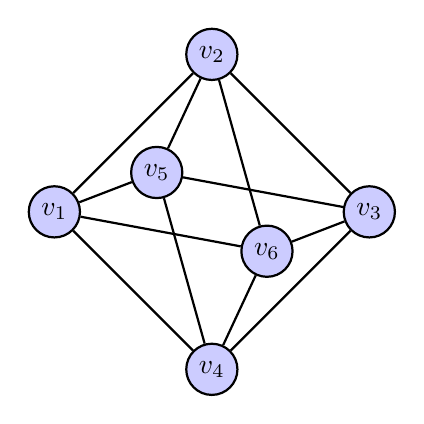
\begin{tikzpicture}[
  scale=1.0,
  vnode/.style={circle, draw=black, fill=blue!20, thick, inner sep=0pt, minimum size=6.5mm},
  edge/.style={thick, draw=black}
]
  % Vértices exteriores (cuadrado C4)
  \node[vnode] (v1) at (-2, 0) {$v_1$};
  \node[vnode] (v2) at (0, 2) {$v_2$};
  \node[vnode] (v3) at (2, 0) {$v_3$};
  \node[vnode] (v4) at (0, -2) {$v_4$};

  % Vértices polo interior/exterior (conectados a todo el C4)
  \node[vnode] (v5) at (-0.7, 0.5) {$v_5$};
  \node[vnode] (v6) at (0.7, -0.5) {$v_6$};

  % Aristas del cuadrado exterior
  \draw[edge] (v1) -- (v2) -- (v3) -- (v4) -- (v1);

  % Conexiones del vértice v5 (polo superior/interior)
  \draw[edge] (v5) -- (v1);
  \draw[edge] (v5) -- (v2);
  \draw[edge] (v5) -- (v3);
  \draw[edge] (v5) -- (v4);

  % Conexiones del vértice v6 (polo inferior/interior)
  \draw[edge] (v6) -- (v1);
  \draw[edge] (v6) -- (v2);
  \draw[edge] (v6) -- (v3);
  \draw[edge] (v6) -- (v4);

\end{tikzpicture}}%
\caption{Un grafo simple}
\end{figure}

En los grafos simples cada arista conecta exactamente dos vértices, de modo que no puede haber aristas que conecten un vértice consigo mismo, ni puede haber más de una arista entre dos vértices. Siguiendo a \cite{Foulds1991}, \cite{Gross2006} y \cite{Pirzada2007}, vemos que, a nivel práctico, los grafos simples son la herramienta estándar para modelar ciertas redes de contactos o relaciones sociales entre personas, organizar la asignación óptima de personal a diferentes tareas y planificar la infraestructura de redes físicas de computadores o servidores. También se utilizan para resolver problemas de asignación de frecuencias en antenas de telefonía móvil evitando interferencias electrónicas, e incluso en biología computacional y ciberseguridad para detectar conflictos genéticos o aislar virus informáticos en servidores clave mediante el análisis de coberturas mínimas. Según las fuentes, la gran ventaja de los grafos simples radica en la limpieza y eficiencia de su estructura. Al no admitir conexiones repetidas ni bucles sobre un mismo punto, pueden almacenarse en computadoras mediante matrices o listas de conexiones muy compactas, lo que mejora significativamente el uso de memoria y a su vez facilita el diseño de algoritmos de búsqueda y optimización extremadamente rápidos.\\\\
Una ligera variante en la noción de grafo simple la presentan los llamados \textit{grafos orientados}. Podemos pensar en un grafo orientado como en un grafo simple en el cual a cada arista se le asigna una ``dirección'', de modo que ahora tenemos registro del vértice del cual ``sale'' una arista y al cual ``llega''. Las aristas son ahora representadas por flechas apuntando desde el vértice de salida al vértice de llegada. Si el grafo orientado $D$ resulta de asignar dirección a las aristas del grafo simple $G$, decimos que $D$ es una \textit{orientación} de G.
\begin{figure}[H]
   \centering
   \resizebox{0.4\textwidth}{!}{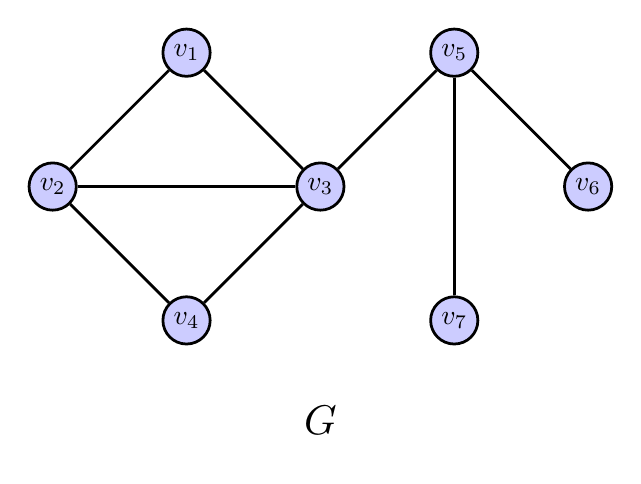
\begin{tikzpicture}[
  scale=0.85, 
  auto=left,
  every node/.style={circle, fill=blue!20, draw=black, line width=1pt, inner sep=2pt, minimum size=6mm}
]

  % Vértices según la disposición del dibujo
  \node (v1) at (2,4) {$v_1$};
  \node (v2) at (0,2) {$v_2$};
  \node (v3) at (4,2) {$v_3$};
  \node (v4) at (2,0) {$v_4$};
  \node (v5) at (6,4) {$v_5$};
  \node (v6) at (8,2) {$v_6$};
  \node (v7) at (6,0) {$v_7$};

  % Aristas de la sección izquierda (entre v1, v2, v3, v4)
  \draw[line width=1pt] (v1) -- (v2);
  \draw[line width=1pt] (v1) -- (v3);
  \draw[line width=1pt] (v2) -- (v3);
  \draw[line width=1pt] (v2) -- (v4);
  \draw[line width=1pt] (v4) -- (v3);

  % Conexión puente (v3 -- v5)
  \draw[line width=1pt] (v3) -- (v5);

  % Aristas de la estrella en v5 (v5 -- v6, v5 -- v7)
  \draw[line width=1pt] (v5) -- (v6);
  \draw[line width=1pt] (v5) -- (v7);

   
  \node[draw=none, fill=none, scale=1.5] at (4,-1.5) {$G$};
\end{tikzpicture}
} \hspace{2em}
   \resizebox{0.4\textwidth}{!}{% Recuerda incluir en el preámbulo:
% \usetikzlibrary{arrows.meta, babel}

\begin{tikzpicture}[
  scale=0.85, 
  auto=left,
  >={Stealth[length=2.5mm]},
  every node/.style={circle, fill=blue!20, draw=black, line width=1pt, inner sep=2pt, minimum size=6mm},
  flecha/.style={->, line width=1pt}
]

  % Vértices según la disposición del dibujo
  \node (v1) at (2,4) {$v_1$};
  \node (v2) at (0,2) {$v_2$};
  \node (v3) at (4,2) {$v_3$};
  \node (v4) at (2,0) {$v_4$};
  \node (v5) at (6,4) {$v_5$};
  \node (v6) at (8,2) {$v_6$};
  \node (v7) at (6,0) {$v_7$};

  % Aristas orientadas del bloque izquierdo
  \draw[flecha] (v2) -- (v1);
  \draw[flecha] (v1) -- (v3);
  \draw[flecha] (v2) -- (v3);
  \draw[flecha] (v2) -- (v4);
  \draw[flecha] (v4) -- (v3);

  % Conexión puente orientada
  \draw[flecha] (v3) -- (v5);

  % Aristas orientadas (v6 -> v5 invertida)
  \draw[flecha] (v6) -- (v5);
  \draw[flecha] (v5) -- (v7);

  \node[draw=none, fill=none, scale=1.5] at (4,-1.5) {$D$};
\end{tikzpicture}
} 
   \caption{$D$ es una orientación de $G$}
\end{figure}
\clearpage
En \cite{Foulds1991} y \cite{Roberts1978} se nos muestra que esta noción de dirección única permite organizar de forma eficiente el flujo vehicular en ciudades mediante calles de un solo sentido sin generar zonas atrapadas o inaccesibles, o representar las jerarquías de victoria y derrota en competencias de tipo ``todos contra todos''. También se nos afirma que el beneficio de un grafo dirigido frente al grafo simple es que añade una jerarquía a las conexiones; sin embargo, al prohibir arcos de ida y vuelta simultáneos entre los mismos dos puntos, conserva una estructura ligera que aún simplifica los cálculos.\\\\
Permitiendo más de una arista entre dos vértices en un grafo orientado, así como aristas de un vértice en sí mismo, obtenemos la noción de \textit{grafo dirigido} o \textit{digrafo}. Las aristas que conectan un mismo par de vértices (sin importar en qué dirección lo hagan) son llamadas \textit{aristas múltiples}. Si un conjunto de aristas múltiples tiene la misma dirección, estas son llamadas \textit{aristas paralelas}. Las aristas que unen un vétice consigo mismo son llamados \textit{bucles}. En la representación de un grafo dirigido solemos curvar ligeramente las aristas múltiples para evitar que estas se superpongan. Ahora, también etiquetamos las aristas del grafo dirigido para poder hacer distinción entre aristas paralelas.
\begin{figure}[H]
  \centering
    \resizebox{0.5\textwidth}{!}{% Recuerda incluir en el preámbulo:
% \usetikzlibrary{arrows.meta, babel}

\begin{tikzpicture}[
  scale=0.85, 
  auto=left,
  >={Stealth[length=2.5mm]},
  every node/.style={circle, fill=blue!20, draw=black, line width=1pt, inner sep=2pt, minimum size=6mm}
]

  % Posicionamiento de vértices
  \node (v1) at (3,6) {$v_1$};
  \node (v2) at (0,4) {$v_2$};
  \node (v3) at (6,4) {$v_3$};
  \node (v4) at (3,3) {$v_4$};
  \node (v5) at (0,1) {$v_5$};
  \node (v6) at (6,1) {$v_6$};
  \node (v7) at (9,1.5) {$v_7$};

  % Bucles en v1 (e1 y e2)
  % e1 bajado un poco más (yshift=-5pt)
  \path[->, line width=1pt] (v1) edge[loop above, out=120, in=60, looseness=8] node[draw=none, fill=none, above] {$e_1$} (v1);
  \path[->, line width=1pt] (v1) edge[loop above, out=150, in=30, looseness=18] node[draw=none, fill=none, above] {$e_2$} (v1);

  % Conexiones v1 <-> v2
  \draw[->, line width=1pt] (v2) to[bend left=15] node[draw=none, fill=none, above] {$e_3$} (v1);
  \draw[->, line width=1pt] (v1) to[bend left=15] node[draw=none, fill=none, below] {$e_4$} (v2);

  % Arista v1 -> v4
  \draw[->, line width=1pt] (v1) -- node[draw=none, fill=none, right] {$e_5$} (v4);

  % Arista v4 -> v5
  \draw[->, line width=1pt] (v4) -- node[draw=none, fill=none, above] {$e_6$} (v5);

  % Bucle en v5 (e7) - Ajustado para alejarlo menos (yshift/xshift reducido a -2pt)
  \path[->, line width=1pt] (v5) edge[loop left, out=210, in=150, looseness=8] node[draw=none, fill=none, xshift=-1pt, yshift=-1pt] {$e_7$} (v5);

  % Múltiples aristas v4 -> v6 (e8, e9, e10)
  \draw[->, line width=1pt] (v4) to[bend left=10] node[draw=none, fill=none, above] {$e_8$} (v6);
  \draw[->, line width=1pt] (v4) to[bend right=25] node[draw=none, fill=none, below] {$e_9$} (v6);
  \draw[->, line width=1pt] (v4) to[bend right=60] node[draw=none, fill=none, below] {$e_{10}$} (v6);

  % Arista v6 -> v4 (e11)
  \draw[->, line width=1pt] (v6) to[bend right=45] node[draw=none, fill=none, above] {$e_{11}$} (v4);

  % Arista v7 -> v3 (e12) - Mantiene orientación horizontal/vertical (sin sloped) y centrada con pos=0.5
  \draw[->, line width=1pt] (v7) -- node[draw=none, fill=none, pos=0.35, above] {$e_{12}$} (v3);

\end{tikzpicture}
} 
  \caption{Un grafo dirigido}
  \label{fig:digrafo}
\end{figure}
En el grafo dirigido de la \Cref{fig:digrafo} podemos señalar, por ejemplo, que $e_1, e_2$ y $e_7$ son bucles, $e_3$ y $e_4$ son aristas múltiples entre $v_1$ y $v_2$, y $e_8,e_9$ y $e_{10}$ son aristas paralelas. Tal como se señala en \cite{Foulds1991}, \cite{Gross2006} y \cite{Roberts1978}, esta flexibilidad hace que los digrafos sean indispensables para coordinar las etapas de proyectos complejos, determinando qué actividades deben terminarse antes de iniciar otras, como reconstruir la secuencia original de fragmentos de ADN o ARN en biología y modelar sistemas con probabilidades de transición entre estados en economía y sociología, por ejemplo. Las fuentes nos muestran que la ventaja de los grafos dirigidos sobre los grafos orientados es que permiten flujos bidireccionales y recorridos que vuelven al mismo punto, algo esencial para representar procesos dinámicos con retroalimentación o ciclos de repetición.\\\\
Si en un grafo dirigido ignoramos la dirección de sus aristas, obtenemos un \textit{multigrafo}.
\begin{figure}[H]
  \centering
  \resizebox{0.45\textwidth}{!}{% Recuerda incluir en el preámbulo:
% \usetikzlibrary{arrows.meta, babel}

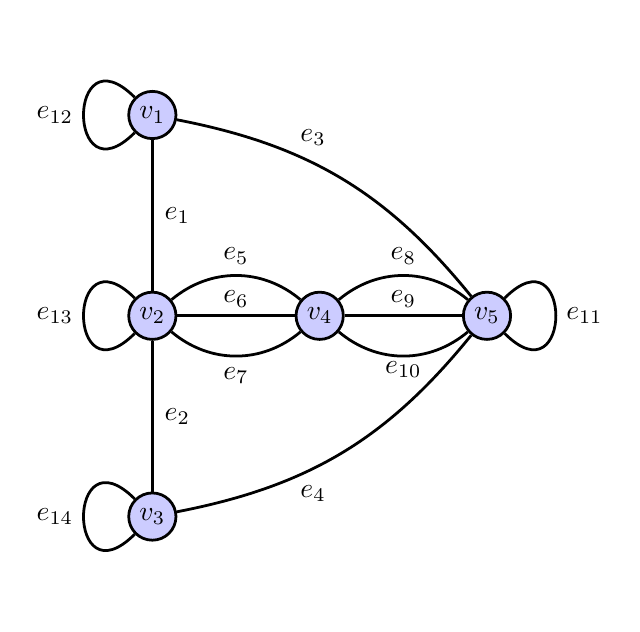
\begin{tikzpicture}[
  scale=0.85, 
  auto=left,
  every node/.style={circle, fill=blue!20, draw=black, line width=1pt, inner sep=2pt, minimum size=6mm}
]

  % Posicionamiento horizontal de vértices
  \node (v1) at (0,3) {$v_1$};
  \node (v3) at (0,-3) {$v_3$};
  \node (v2) at (0,0) {$v_2$};
  \node (v4) at (2.5,0) {$v_4$};
  \node (v5) at (5,0) {$v_5$};

  % Bucles en v1, v2 y v3
  \path[line width=1pt] (v1) edge[loop left, out=135, in=225, looseness=7] node[draw=none, fill=none, left, inner sep=2pt] {$e_{12}$} (v1);
  \path[line width=1pt] (v2) edge[loop left, out=135, in=225, looseness=7] node[draw=none, fill=none, left, inner sep=2pt] {$e_{13}$} (v2);
  \path[line width=1pt] (v3) edge[loop left, out=135, in=225, looseness=7] node[draw=none, fill=none, left, inner sep=2pt] {$e_{14}$} (v3);

  % Aristas verticales iniciales
  \draw[line width=1pt] (v1) -- node[draw=none, fill=none, right, inner sep=1pt] {$e_1$} (v2);
  \draw[line width=1pt] (v2) -- node[draw=none, fill=none, right, inner sep=1pt] {$e_2$} (v3);

  % Conexiones curvas v1 -> v5 y v3 -> v5
  \draw[line width=1pt] (v1) to[bend left=20] node[draw=none, fill=none, above, inner sep=1pt, pos=0.4] {$e_3$} (v5);
  \draw[line width=1pt] (v3) to[bend right=20] node[draw=none, fill=none, below, inner sep=1pt, pos=0.4] {$e_4$} (v5);

  % Múltiples aristas entre v2 y v4
  \draw[line width=1pt] (v2) to[bend left=40] node[draw=none, fill=none, above, yshift=-2pt] {$e_5$} (v4);
  \draw[line width=1pt] (v2) -- node[draw=none, fill=none, above, yshift=-3pt] {$e_6$} (v4);
  \draw[line width=1pt] (v2) to[bend right=40] node[draw=none, fill=none, below, yshift=2pt] {$e_7$} (v4);

  % Múltiples aristas entre v4 y v5
  \draw[line width=1pt] (v4) to[bend left=40] node[draw=none, fill=none, above, yshift=-2pt] {$e_8$} (v5);
  \draw[line width=1pt] (v4) -- node[draw=none, fill=none, above, yshift=-3pt] {$e_9$} (v5);
  \draw[line width=1pt] (v4) to[bend right=40] node[draw=none, fill=none, below, yshift=5.5pt] {$e_{10}$} (v5);

  % Bucle en v5
  \path[line width=1pt] (v5) edge[loop right, out=45, in=-45, looseness=7] node[draw=none, fill=none, right, pos=0.5, inner sep=2pt] {$e_{11}$} (v5);

\end{tikzpicture}
} 
  \caption{Un multigrafo}
  \label{fig:multigrafo}
\end{figure}
En un multigrafo aún se permiten aristas múltiples entre vértices, así como bucles. En el multigrafo de la \Cref{fig:multigrafo} podemos ver, por ejemplo, que $e_8,e_9$ y $e_{10}$ son aristas múltiples entre $v_4$ y $v_5$, que $e_{12}$ es un bucle sobre $v_1$ y que $e_{14}$ es un bucle sobre $v_3$. De acuerdo con \cite{Andrei2008}, \cite{Butler2023}, \cite{Gross2006} y \cite{Shafie2012}, los multigrafos se aplican con éxito en el análisis de redes sociales para estudiar simultáneamente distintos tipos de lazos entre las mismas personas (como amistad, trabajo o préstamos de dinero), en la representación de redes de transporte con varias alternativas paralelas (como tren y autobús entre dos estaciones) y en química, para describir enlaces moleculares múltiples, entre otros. Se menciona que la principal ventaja de los multigrafos reside en que pueden registrar varios canales de interacción al mismo tiempo, sin necesidad de simplificarlos o fusionarlos en un solo enlace, preservando la riqueza del fenómeno real.\clearpage
Si ahora permitimos que las aristas sean subconjuntos de vértices no vacíos, y de cualquier cardinalidad, obtenemos la noción de \textit{hipergrafo}. Las aristas de un hipergrafo se representan como diagramas de Venn, encerrando únicamente los vértices que contiene.
\begin{figure}[H]
  \centering
    \resizebox{0.6\textwidth}{!}{% Recuerda incluir en el preámbulo:
% \usetikzlibrary{babel}

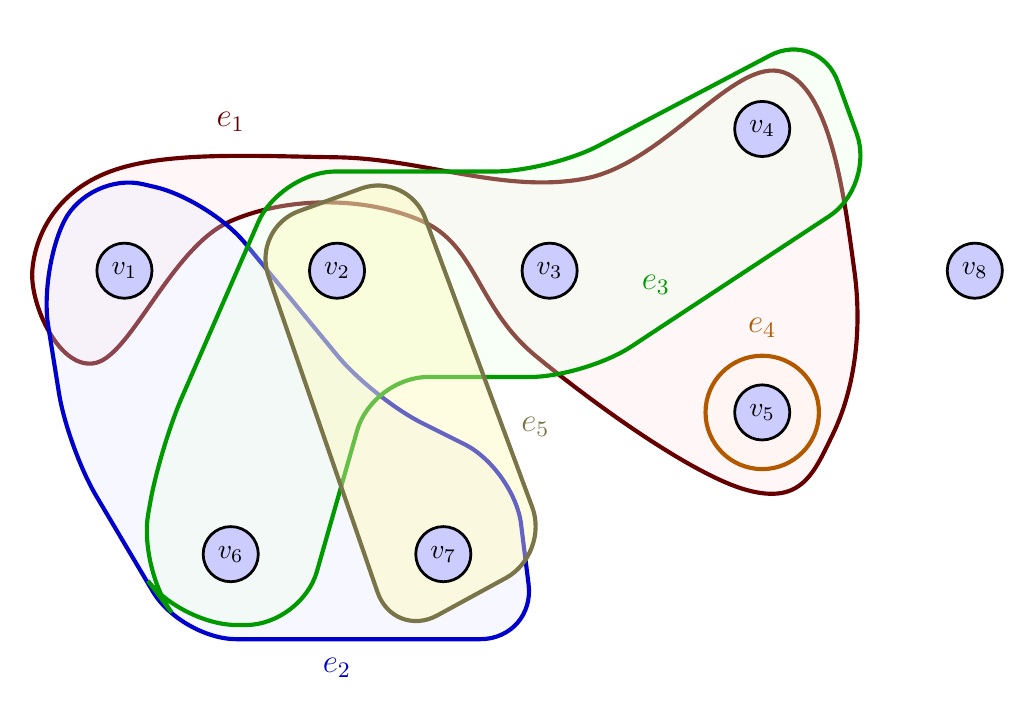
\begin{tikzpicture}[
  scale=0.9,
  every node/.style={circle, fill=blue!20, draw=black, line width=1pt, inner sep=2pt, minimum size=7mm}
]

  % ==========================================
  % 1. HIPERARISTAS (dibujadas al fondo)
  % ==========================================
  
  % e1 = {v1, v3, v4, v5} (Rojo oscuro - trazado orgánico y suave)
  \draw[red!40!black, line width=1.5pt, fill=red!10, fill opacity=0.3]
    plot [smooth cycle, tension=0.65] coordinates {
      (-1.3, 3.0)
      (-0.2, 4.4)
      (3.0, 4.6)
      (6.5, 4.3)
      (9.3, 5.8)
      (10.3, 3.0)
      (10.0, 0.7)
      (8.8, -0.1)
      (5.8, 1.8)
      (4.2, 3.7)
      (1.5, 3.7)
      (-0.4, 1.7)
    };
  \node[draw=none, fill=none, red!40!black, font=\large] at (1.5, 5.1) {$e_1$};

  % e2 = {v1, v6, v7} (Azul)
  \draw[blue!80!black, line width=1.5pt, fill=blue!10, fill opacity=0.3, rounded corners=20pt]
    (-1.2, 3) -- (-0.5, 4.4) -- (1.2, 4) -- (3.5, 1.2) -- (5.5, 0.2) -- 
    (5.8, -2.2) -- (0.8, -2.2) -- (-0.8, 0.5) -- cycle;
  \node[draw=none, fill=none, blue!80!black, font=\large] at (3, -2.6) {$e_2$};

  % e3 = {v2, v3, v4, v6} (Verde)
  \draw[green!60!black, line width=1.5pt, fill=green!10, fill opacity=0.3, rounded corners=20pt]
    (0.2, -1.2) -- (0.5, 0.5) -- (2.2, 4.4) -- (6, 4.4) -- (9.8, 6.4) -- 
    (10.6, 4.2) -- (6.5, 1.5) -- (3.5, 1.5) -- (2.5, -2) -- (0.8, -2) -- cycle;
  \node[draw=none, fill=none, green!60!black, font=\large] at (7.5, 2.8) {$e_3$};

  % e5 = {v2, v7} (Amarillo oscuro/Dorado)
  \draw[yellow!40!black, line width=1.5pt, fill=yellow!30, fill opacity=0.4, rounded corners=18pt]
    (1.8, 3.6) -- (4, 4.4) -- (6, -1) -- (3.8, -2.2) -- cycle;
  \node[draw=none, fill=none, yellow!40!black, font=\large] at (5.8, 0.8) {$e_5$};

  % e4 = {v5} (Naranja)
  \draw[orange!70!black, line width=1.5pt, fill=orange!10, fill opacity=0.3]
    (9,1) circle (8mm);
  \node[draw=none, fill=none, orange!70!black, font=\large] at (9, 2.2) {$e_4$};


  % ==========================================
  % 2. VÉRTICES (dibujados sobre las áreas)
  % ==========================================
  \node (v1) at (0,3) {$v_1$};
  \node (v2) at (3,3) {$v_2$};
  \node (v3) at (6,3) {$v_3$};
  \node (v4) at (9,5) {$v_4$};
  \node (v5) at (9,1) {$v_5$};
  \node (v6) at (1.5,-1) {$v_6$};
  \node (v7) at (4.5,-1) {$v_7$};
  \node (v8) at (12,3) {$v_8$};

\end{tikzpicture}
} 
  \caption{Un hipergrafo}
\end{figure}
Según lo señalado en \cite{Bretto2013} y \cite{Molnar2014}, los hipergrafos son muy útiles en informática para diseñar y organizar grandes bases de datos relacionales, coordinar horarios concurrentes sin solapamientos y analizar colaboraciones de grupo en redes de personas (como comités o artículos científicos escritos por múltiples autores). Nos muestran que el máximo beneficio de este tipo de grafos radica en romper la barrera del enlace por parejas, agrupando a un número arbitrario de participantes en una misma relación e independizando al modelo de simplificaciones bidireccionales o binarias artificiales.

\subsection{Conceptos básicos}
En el presente estudio trabajaremos únicamente con grafos simples, así que de ahora en adelante se entenderá \textit{grafo} y \textit{grafo simple} de manera indistinta. Iniciamos formalizando la noción de grafo que hemos introducido. Las definiciones presentadas en lo que sigue de esta sección son estándar en la teoría; las tomamos siguiendo a \cite{diestel2017}, \cite{gomez2025} y \cite{jafarian2013}.
\begin{Not}
Dado un conjunto $S$ y un número natural $k$, denotamos por $[S]^k$ a la colección de todos los subconjuntos de $S$ con exactamente $k$ elementos.
\end{Not}\clearpage
Así por ejemplo, tomando $S=\left\lbrace 1,2,3,4,5 \right\rbrace$, tenemos que 
$$
\begin{aligned}
   [S]^3 &= \left\lbrace \left\lbrace 1,2,3\right\rbrace, \left\lbrace 1,2,4\right\rbrace, \left\lbrace 1,2,5\right\rbrace, \left\lbrace 1,3,4\right\rbrace, \left\lbrace 1,3,5\right\rbrace, \left\lbrace 1,4,5\right\rbrace, \left\lbrace 2,3,4\right\rbrace, \left\lbrace 2,3,5\right\rbrace \right.,\\
         &\phantom{ooo} \left. \left\lbrace 2,4,5\right\rbrace, \left\lbrace 3,4,5\right\rbrace\right\rbrace. 
\end{aligned}
$$
Los elementos de $[S]^k$ son llamados $k-subconjuntos$ de $S$. Con esto, damos la definición de grafo.
\begin{Def}
   Un \textbf{grafo} (simple) es una pareja $G=\left( V,E\right)$ de conjuntos tales que $E\subseteq [V]^2$. Los elementos de $V$ son llamados \textbf{vértices} y los elementos de $E$ son llamados \textbf{aristas}.
\end{Def}
De este modo, las aristas de un grafo son $2-subconjuntos$ de vértices. Si es necesario, dado un grafo $G$, también se denota por $V(G)$ a su conjunto de vértices, y por $E(G)$ a su conjunto de aristas. Un grafo con conjunto de vértices $V$ también es llamado un \textit{grafo sobre V}. Para evitar ambiguedades de notación, asumimos también que $V(G)\cap E(G)=\emptyset$ para todo grafo $G$. Una arista $\left\lbrace u,v\right\rbrace$ de un grafo también puede ser representada mediante $uv$. Una manera estándar y conveniente de representar visualmente un grafo es dibujar un círculo o punto por cada vértice, y unir dos de estos círculos por una línea si y sólo si los correspondientes vértices forman una arista del grafo. La distribución particular de los círculos en el espacio, así como la forma en que las líneas son dibujadas es irrelevante; la única información que importa es qué par de vértices están conectados mediante una arista y cuáles no. Solemos referirnos por \textit{grafo} también a la respectiva representación visual.
\begin{Ejm} \label{Ejm:cuatro_grafos}
   Los siguientes son ejemplos de grafos sobre $V=\left\lbrace v_1,v_2,v_3,v_4,v_5, v_6 \right\rbrace$:
  \phantom{o}\\
{\centering
  % ================= FILA 1 =================
  \makebox[0.48\textwidth][c]{%
    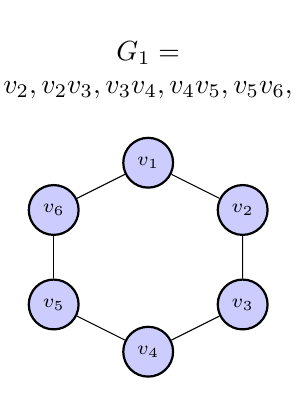
\begin{tikzpicture}
  [scale=.6, auto=left, 
   vertex/.style={circle, fill=blue!20, draw=black, thick, inner sep=2pt, minimum size=18pt}]

  \node[vertex] (n1) at (2,4) {$\scriptstyle v_1$};
  \node[vertex] (n2) at (4,3) {$\scriptstyle v_2$};
  \node[vertex] (n3) at (4,1) {$\scriptstyle v_3$};
  \node[vertex] (n4) at (2,0) {$\scriptstyle v_4$};
  \node[vertex] (n5) at (0,1) {$\scriptstyle v_5$};
  \node[vertex] (n6) at (0,3) {$\scriptstyle v_6$};

  \foreach \from/\to in {n1/n2,n2/n3,n3/n4,n4/n5,n5/n6,n6/n1}
    \draw (\from) -- (\to);

  \node[anchor=south, yshift=0.3cm] at (n1.north) {%
    \makebox[0pt][c]{%
      $\begin{array}{c}
        G_1=\\
        (V,\{v_1v_2,v_2v_3,v_3v_4,v_4v_5,v_5v_6, v_6v_1\})
      \end{array}$%
    }%
  };
\end{tikzpicture}
%
  }%
  \hfill
  \makebox[0.48\textwidth][c]{%
    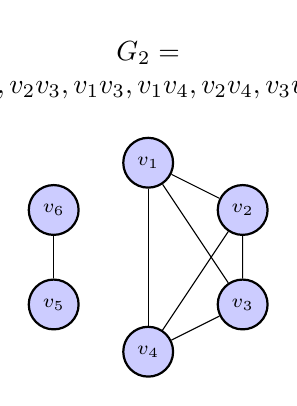
\begin{tikzpicture}
  [scale=.6, auto=left, 
   vertex/.style={circle, fill=blue!20, draw=black, thick, inner sep=2pt, minimum size=18pt}]

  \node[vertex] (n1) at (2,4) {$\scriptstyle v_1$};
  \node[vertex] (n2) at (4,3) {$\scriptstyle v_2$};
  \node[vertex] (n3) at (4,1) {$\scriptstyle v_3$};
  \node[vertex] (n4) at (2,0) {$\scriptstyle v_4$};
  \node[vertex] (n5) at (0,1) {$\scriptstyle v_5$};
  \node[vertex] (n6) at (0,3) {$\scriptstyle v_6$};

  \foreach \from/\to in {n1/n2,n2/n3,n1/n3, n1/n4, n2/n4, n3/n4,n5/n6}
    \draw (\from) -- (\to);

  \node[anchor=south, yshift=0.3cm] at (n1.north) {%
    \makebox[0pt][c]{%
      $\begin{array}{c}
        G_2=\\
        (V,\{v_1v_2, v_2v_3, v_1v_3, v_1v_4, v_2v_4, v_3v_4, v_5v_6\})
      \end{array}$%
    }%
  };
\end{tikzpicture}
%
  }\par

  \vspace{1.5em}% Separación vertical entre filas de diagramas

  % ================= FILA 2 =================
  \makebox[0.48\textwidth][c]{%
    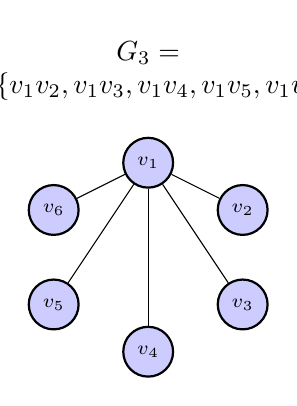
\begin{tikzpicture}
  [scale=.6, auto=left, 
   vertex/.style={circle, fill=blue!20, draw=black, thick, inner sep=2pt, minimum size=18pt}]

  \node[vertex] (n1) at (2,4) {$\scriptstyle v_1$};
  \node[vertex] (n2) at (4,3) {$\scriptstyle v_2$};
  \node[vertex] (n3) at (4,1) {$\scriptstyle v_3$};
  \node[vertex] (n4) at (2,0) {$\scriptstyle v_4$};
  \node[vertex] (n5) at (0,1) {$\scriptstyle v_5$};
  \node[vertex] (n6) at (0,3) {$\scriptstyle v_6$};

  \foreach \from/\to in {n1/n2, n1/n3, n1/n4, n1/n5, n1/n6}
    \draw (\from) -- (\to);

  \node[anchor=south, yshift=0.3cm] at (n1.north) {%
    \makebox[0pt][c]{%
      $\begin{array}{c}
        G_3=\\
        (V, \{v_1v_2, v_1v_3, v_1v_4, v_1v_5, v_1v_6\})
      \end{array}$%
    }%
  };
\end{tikzpicture}
%
  }%
  \hfill
  \makebox[0.48\textwidth][c]{%
    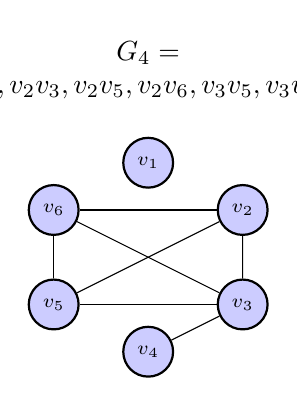
\begin{tikzpicture}
  [scale=.6, auto=left, 
   vertex/.style={circle, fill=blue!20, draw=black, thick, inner sep=2pt, minimum size=18pt}]

  \node[vertex] (n1) at (2,4) {$\scriptstyle v_1$};
  \node[vertex] (n2) at (4,3) {$\scriptstyle v_2$};
  \node[vertex] (n3) at (4,1) {$\scriptstyle v_3$};
  \node[vertex] (n4) at (2,0) {$\scriptstyle v_4$};
  \node[vertex] (n5) at (0,1) {$\scriptstyle v_5$};
  \node[vertex] (n6) at (0,3) {$\scriptstyle v_6$};

  \foreach \from/\to in {n3/n4,n2/n3, n2/n5, n2/n6, n3/n5, n3/n6, n5/n6}
    \draw (\from) -- (\to);

  \node[anchor=south, yshift=0.3cm] at (n1.north) {%
    \makebox[0pt][c]{%
      $\begin{array}{c}
        G_4=\\
        (V,\{v_3v_4, v_2v_3, v_2v_5, v_2v_6, v_3v_5, v_3v_6, v_5v_6\})
      \end{array}$%
    }%
  };
\end{tikzpicture}
%
  }\par

  \vspace{1.2em}% Espacio entre los diagramas y el título/caption
  \captionof{figure}{Ejemplos de grafos sobre $V$}
  \label{fig:ejemplos_grafos_conjuntos}
\par}
\phantom{o}\\

   Un ejemplo de grafo sobre $V'=\left\lbrace v_1, v_2, v_3, \dots\right\rbrace$ es $G_5=(V',\left\lbrace v_1v_2, v_2v_3, v_3v_4, v_4v_5, \dots\right\rbrace)$.
   \begin{figure}[H]
     \centering
       \resizebox{0.45\textwidth}{!}{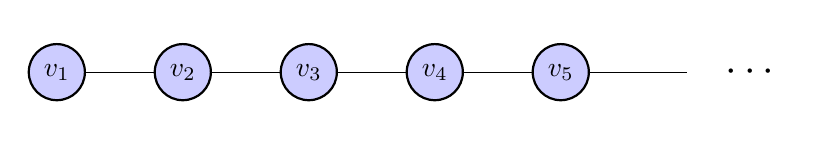
\begin{tikzpicture}
  [scale=.8,auto=left,every node/.style={circle,fill=blue!20,draw=black,thick}]
  \node (n1) at (0,0) {$v_1$};
  \node (n2) at (2,0)  {$v_2$};
  \node (n3) at (4,0)  {$v_3$};
  \node (n4) at (6,0) {$v_4$};
  \node (n5) at (8,0)  {$v_5$};

  \foreach \from/\to in {n1/n2,n2/n3, n3/n4, n4/n5}
    \draw (\from) -- (\to);

   %Flecha de (n5) a un nodo invisible en (10,0)   
   \draw (n5) -- (10,0);
   
   %Etiqueta de puntos suspensivos
   \node[draw=none, fill=none, scale=1.5] at (11,0) {$\cdots$};
   % Etiqueta G_1 debajo del grafo
%   \node[draw=none, fill=none, scale=1.5] at (6,-1.5) {$G_5$};
\end{tikzpicture}
} 
     \caption{El grafo $G_5$ sobre $V'$}
   \end{figure}
\end{Ejm}
\begin{Not}
   El grafo $G=(\emptyset,\emptyset)$ en el cual tanto el conjunto de vértices como el de aristas son vacíos, lo llamamos \textbf{grafo vacío} y lo representamos simplemente por $\emptyset$.
\end{Not}
Notemos que en un grafo $G$, dada $uv\in E(G)$, se tiene que $uv$ y $vu$ hacen referencia a la misma arista, pues $uv=\left\lbrace u,v \right\rbrace=\left\lbrace v, u\right\rbrace=vu$. De esta forma, en un grafo, el orden de los vértices en la representación de una arista no es tenido en cuenta, lo cual está alineado con nuestra idea de no considerar orientación en ella. Además, la exigencia de que las aristas de un grafo sean $2-subconjuntos$ de vértices implica que si $uv\in E(G)$ entonces $u\neq v$, es decir, no hay aristas que unan un vértice con sí mismo, de modo que los grafos que consideramos no tienen bucles. Así mismo, entre dos vértices distintos $u,v\in V(G)$ podrá haber a lo más una arista, dependiendo de si $uv$ pertenece a $E(G)$ o no, es decir, se excluye la posibilidad de que hayan aristas múltiples entre un par de vértices.\par
Frecuentemente en matemáticas, uno de los primeros pasos al analizar una estructura formal es estudiar sus subestructuras, es decir, objetos del mismo tipo contenidos en ella. Para esto introducimos la noción de \textit{subgrafo}.\clearpage
\begin{Def}
   Dados dos grafos $G=(V,E)$ y $G'=(V',E')$, decimos que $G'$ es un \textbf{subgrafo} de $G$ si $V'\subseteq V$ y $E'\subseteq E$. En este caso denotamos $G'\subseteq G$.
\end{Def}
Para cualquier grafo $G$ se tiene $\emptyset\subseteq G$. Damos a continuación más ejemplos de contenencia de grafos.
\begin{Ejm}\label{Ejm:Contenencia}
   En cada fila de la \Cref{tab:grafos} se tiene $G'\subseteq G$.
   \par\vspace{1em}
\begin{longtable}{|c|c|c|}
  \hline
  \rule[-0.5em]{0pt}{1.8em} & \rule[-0.5em]{0pt}{1.8em} $G$ & \rule[-0.5em]{0pt}{1.8em} $G'$ \\
  \hline
  \endhead
  \hline
  \endfoot
  \caption{Ejemplos de contenencia de grafos} \addtocounter{table}{-1}\refstepcounter{table}\label{tab:grafos} \\
  \endlastfoot

  $G_1 \subseteq G'_1$ &
  \begin{minipage}{0.3\textwidth} \centering \vspace{8pt} \resizebox{0.85\linewidth}{!}{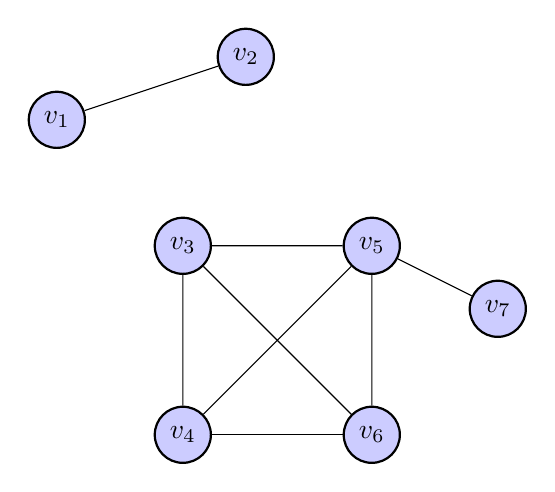
\begin{tikzpicture}
   [scale=.8,auto=left,every node/.style={circle,fill=blue!20,draw=black,thick}]
  \node (n1) at (0,5) {$v_1$};
  \node (n2) at (3,6) {$v_2$};
  \node (n3) at (2,3) {$v_3$};
  \node (n4) at (2,0) {$v_4$};
  \node (n5) at (5,3) {$v_5$};
  \node (n6) at (5,0) {$v_6$};
  \node (n7) at (7,2) {$v_7$};

  \foreach \from/\to in {n1/n2, n3/n5, n5/n6, n6/n4, n4/n3, n3/n6, n4/n5, n5/n7}
    \draw (\from) -- (\to);

\end{tikzpicture}
} \vspace{6pt} \end{minipage} &
  \begin{minipage}{0.3\textwidth} \centering \vspace{8pt} \resizebox{0.85\linewidth}{!}{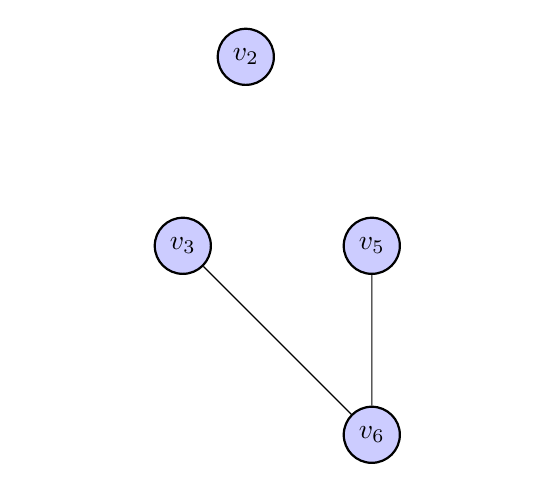
\begin{tikzpicture}
  [scale=.8,auto=left,every node/.style={circle,fill=blue!20,draw=black,thick}]
  \node (n1) at (0,5) [opacity=0] {$v_1$};
  \node (n2) at (3,6) {$v_2$};
  \node (n3) at (2,3) {$v_3$};
  \node (n4) at (2,0) [opacity=0]{$v_4$};
  \node (n5) at (5,3) {$v_5$};
  \node (n6) at (5,0) {$v_6$};
  \node (n7) at (7,2) [opacity=0]{$v_7$};

  \foreach \from/\to in {n1/n2, n3/n5, n5/n6, n6/n4, n4/n3, n3/n6, n4/n5, n5/n7}
    \draw[opacity=0] (\from) -- (\to);
   
    \foreach \from/\to in {n3/n6, n5/n6}
     \draw[opacity=1] (\from) -- (\to);

  \end{tikzpicture}
} \vspace{6pt} \end{minipage} \\
  \hline

  $G_2 \subseteq G'_2$ &
  \begin{minipage}{0.3\textwidth} \centering \vspace{8pt} \resizebox{0.8\linewidth}{!}{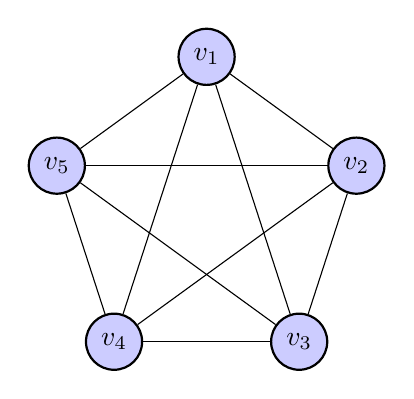
\begin{tikzpicture}
  [scale=1,auto=left,every node/.style={circle,fill=blue!20,draw=black,thick}]
  \node (n1) at (90:2) {$v_1$};
  \node (n2) at (18:2) {$v_2$};
  \node (n3) at (-54:2) {$v_3$};
  \node (n4) at (-126:2) {$v_4$};
  \node (n5) at (-198:2) {$v_5$};

  \foreach \from/\to in {n1/n2, n1/n3, n1/n4, n1/n5, n2/n3, n2/n4, n2/n5, n3/n4, n3/n5, n4/n5}
    \draw (\from) -- (\to);

 \end{tikzpicture}
} \vspace{6pt} \end{minipage} &
  \begin{minipage}{0.3\textwidth} \centering \vspace{8pt} \resizebox{0.8\linewidth}{!}{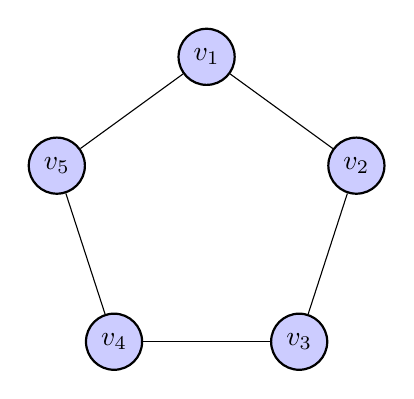
\begin{tikzpicture}
  [scale=1,auto=left,every node/.style={circle,fill=blue!20,draw=black,thick}]
  \node (n1) at (90:2) {$v_1$};
  \node (n2) at (18:2) {$v_2$};
  \node (n3) at (-54:2) {$v_3$};
  \node (n4) at (-126:2) {$v_4$};
  \node (n5) at (-198:2) {$v_5$};

  \foreach \from/\to in {n1/n2, n2/n3, n3/n4, n4/n5, n5/n1}
    \draw (\from) -- (\to);

 \end{tikzpicture}
} \vspace{6pt} \end{minipage} \\
  \hline

  $G_3 \subseteq G'_3$ &
  \begin{minipage}{0.3\textwidth} \centering \vspace{8pt} \resizebox{0.8\linewidth}{!}{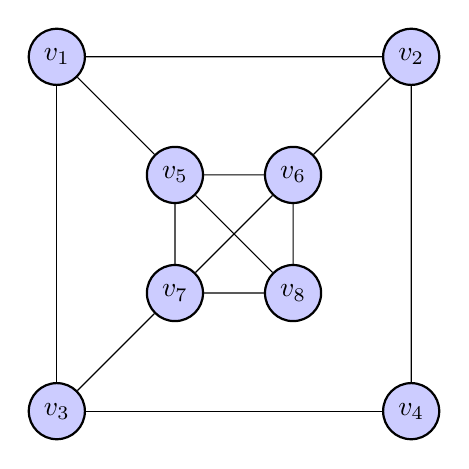
\begin{tikzpicture}
  [scale=1.5,auto=left,every node/.style={circle,fill=blue!20,draw=black,thick}]
  \node (n1) at (0,3) {$v_1$};
  \node (n2) at (3,3) {$v_2$};
  \node (n3) at (0,0) {$v_3$};
  \node (n4) at (3,0) {$v_4$};
  \node (n5) at (1,2) {$v_5$};
  \node (n6) at (2,2) {$v_6$};
  \node (n7) at (1,1) {$v_7$};
  \node (n8) at (2,1) {$v_8$};

  \foreach \from/\to in {n1/n2, n1/n3, n2/n4, n3/n7, n6/n7, n1/n5, n2/n6, n5/n6, n6/n8, n7/n8, n7/n5, n5/n8, n3/n4}
    \draw (\from) -- (\to);

 \end{tikzpicture}
} \vspace{6pt} \end{minipage} &
  \begin{minipage}{0.3\textwidth} \centering \vspace{8pt} \resizebox{0.8\linewidth}{!}{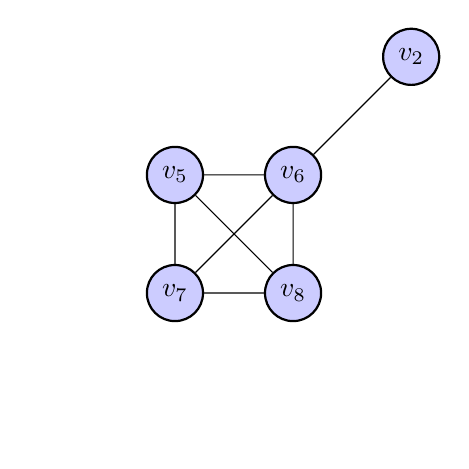
\begin{tikzpicture}
  [scale=1.5,auto=left,every node/.style={circle,fill=blue!20,draw=black,thick}]
  \node (n1) at (0,3) [opacity=0] {$v_1$};
  \node (n2) at (3,3) {$v_2$};
  \node (n3) at (0,0) [opacity=0] {$v_3$};
  \node (n4) at (3,0) [opacity=0] {$v_4$};
  \node (n5) at (1,2) {$v_5$};
  \node (n6) at (2,2) {$v_6$};
  \node (n7) at (1,1) {$v_7$};
  \node (n8) at (2,1) {$v_8$};

  \foreach \from/\to in {n2/n6, n5/n6, n6/n8, n7/n8, n7/n5, n5/n8, n6/n7}
    \draw (\from) -- (\to);

 \end{tikzpicture}
} \vspace{6pt} \end{minipage} \\
  \hline
\end{longtable}
\par\vspace{-0.3em}

\end{Ejm}\clearpage
En el \Cref{Ejm:Contenencia} se cumple que $G'_3$ conserva todas las aristas entre vértices de $V(G'_3)$ que aparecían originalmente en $G_3$, es decir, para cualesquiera $u,v\in V(G'_3)$ se tiene que $uv\in E(G_3)$ implica $uv\in E(G'_3)$. Notemos que en los ejemplos $G_1$ y $G_2$ esto no se cumple. Por ejemplo, para $G_1$ se tiene $v_3,v_5\in V(G'_1)$ y $v_3v_5\in E(G_1)$, pero $v_3v_5 \notin E(G'_1)$; para $G_2$ se tiene $v_1,v_3\in V(G'_2)$ y $v_1v_3\in E(G_2)$, pero $v_1v_3\notin E(G'_2)$. El comportamiento que se da con $G_3$ y $G'_3$ lo resumimos diciendo que $G'_3$ es el \textit{subgrafo de $G_3$ inducido} por $V(G'_3)$, y denotamos $G'_3=G[V(G'_3)]$. Más precisamente:
\begin{Def}
   Sean $G$ un grafo y $W\subseteq V(G)$. El \textbf{subgrafo de $G$ inducido} por $W$, denotado por $G[W]$, se define como el subgrafo de $G$ tal que $V(G[W])=W$ y $E(G[W])=\left\lbrace uv\in E(G)\mid u,v\in W\right\rbrace$.
\end{Def}
\begin{Ejm}
   \phantom{o}
   \begin{itemize}
      \item $G_2$ es el subgrafo de $G_1$ inducido por $W=\left\lbrace v_2,v_3,v_4,v_5,v_6\right\rbrace$:
         \begin{figure}[H]
  \centering
  \resizebox{0.2\textwidth}{!}{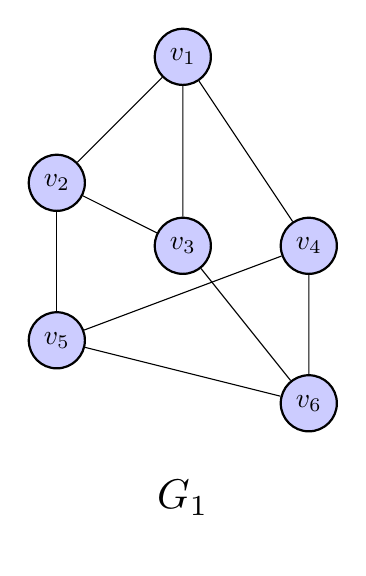
\begin{tikzpicture}
  [scale=.8,auto=left,every node/.style={circle,fill=blue!20,draw=black,thick}]
  \node (n1) at (3,6) {$v_1$};
  \node (n2) at (1,4) {$v_2$};
  \node (n3) at (3,3) {$v_3$};
  \node (n4) at (5,3) {$v_4$};
  \node (n5) at (1,1.5) {$v_5$};
  \node (n6) at (5,0.5) {$v_6$};

  \foreach \from/\to in {n1/n2, n1/n3, n1/n4, n2/n3, n2/n5, n3/n6, n4/n5, n4/n6, n5/n6}
    \draw (\from) -- (\to);

   \node[draw=none, fill=none, scale=1.5] at (3,-1) {$G_1$};
\end{tikzpicture}
} \hspace{2cm}
    \resizebox{0.2\textwidth}{!}{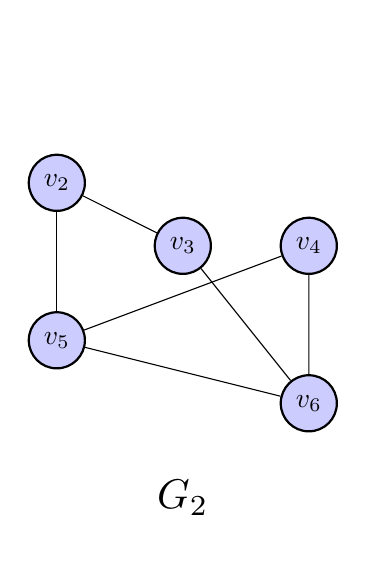
\begin{tikzpicture}
  [scale=.8,auto=left,every node/.style={circle,fill=blue!20,draw=black,thick}]
  \node (n1) at (3,6) [opacity=0] {$v_1$};
  \node (n2) at (1,4) {$v_2$};
  \node (n3) at (3,3) {$v_3$};
  \node (n4) at (5,3) {$v_4$};
  \node (n5) at (1,1.5) {$v_5$};
  \node (n6) at (5,0.5) {$v_6$};

  \foreach \from/\to in {n2/n3, n2/n5, n3/n6, n4/n5, n4/n6, n5/n6}
    \draw (\from) -- (\to);


   \node[draw=none, fill=none, scale=1.5] at (3,-1) {$G_2$};
\end{tikzpicture}
} 
    \caption{$G_2=G_1[W]$}
\end{figure}
  
      \item $G_4$ es el subgrafo de $G_3$ inducido por $W'=\left\lbrace v_1,v_2,v_3,v_5\right\rbrace$:
         \vspace{-4em}
\begin{figure}[H]
  \hspace*{3.9cm}%
  \resizebox{0.23\textwidth}{!}{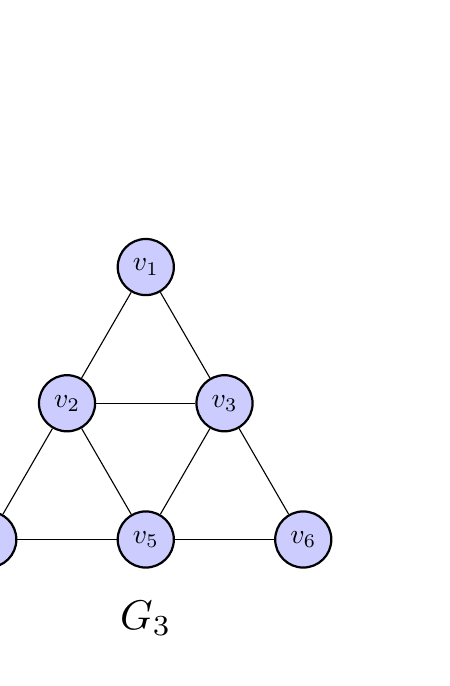
\begin{tikzpicture}
  [scale=1,auto=left,every node/.style={circle,fill=blue!20,draw=black,thick}]
\useasboundingbox (0.5,-1.5) rectangle (5.5,6.5);
  % Posiciones simétricas en forma de triángulo equilátero
  \node (n1) at (2,3.46) {$v_1$};
  \node (n2) at (1,1.73) {$v_2$};
  \node (n3) at (3,1.73) {$v_3$};
  \node (n4) at (0,0)    {$v_4$};
  \node (n5) at (2,0)    {$v_5$};
  \node (n6) at (4,0)    {$v_6$};

  % Aristas del grafo base (malla triangular)
  \foreach \from/\to in {n1/n2, n1/n3, n2/n3, n2/n4, n2/n5, n3/n5, n3/n6, n4/n5, n5/n6}
    \draw (\from) -- (\to);

   \node[draw=none, fill=none, scale=1.5] at (2,-1) {$G_3$};
\end{tikzpicture}
}
  \hspace*{1.15cm}
    \resizebox{0.23\textwidth}{!}{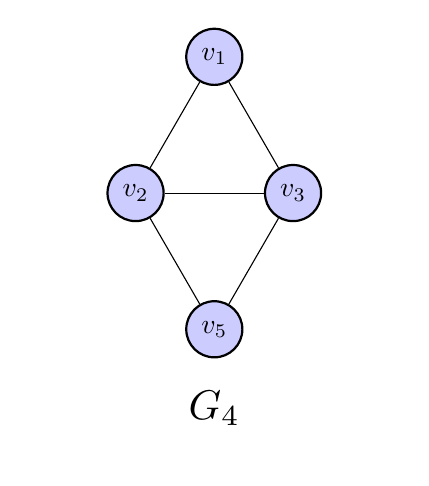
\begin{tikzpicture}
  [scale=1,auto=left,every node/.style={circle,fill=blue!20,draw=black,thick}]
  % Posiciones simétricas en forma de triángulo equilátero
  \node (n1) at (2,3.46) {$v_1$};
  \node (n2) at (1,1.73) {$v_2$};
  \node (n3) at (3,1.73) {$v_3$};
  \node (n4) at (0,0)   [opacity=0] {$v_4$};
  \node (n5) at (2,0)    {$v_5$};
  \node (n6) at (4,0)   [opacity=0] {$v_6$};

  % Aristas del grafo base (malla triangular)
  \foreach \from/\to in {n1/n2, n1/n3, n2/n3, n2/n5, n3/n5}
    \draw (\from) -- (\to);

   \node[draw=none, fill=none, scale=1.5] at (2,-1) {$G_4$};
\end{tikzpicture}
} 
    \caption{$G_4=G_3[W']$}
\end{figure}
  
   \end{itemize}
\end{Ejm}
\begin{Def}
   El \textbf{orden} de un grafo $G$, representado mediante $|G|$, es el cardinal del conjunto $V(G)$.
\end{Def}
Así, en el \Cref{Ejm:cuatro_grafos}, el grado de los cuatro primeros grafos es $6$, mientras que $|G_5|=\aleph _0$. Los grafos pueden ser \textit{finitos, infinitos, contables}, etc., dependiendo del respectivo tamaño del conjunto $G$.
\begin{Def}
   Dado un grafo $G$, decimos que dos vértices $u,v\in V(G)$ son \textbf{adyacentes} si $uv\in E(G)$. Igualmente, decimos que el vértice $v\in V(G)$ es \textbf{incidente} con la arista $e\in E(G)$ si $v\in e$. 
\end{Def}
En el grafo $G_1$ del \Cref{Ejm:cuatro_grafos}, los vértices $v_3$ y $v_4$ son adyacentes, los vértices $v_2$ y $v_5$ no son adyacentes, el vértice $v_6$ es incidente con la arista $v_1v_6$ y el vértice $v_4$ no es incidente con la arista $v_2v_3$. Los grafos finitos permiten una representación mediante matrices basada en las relaciones de adyacencia de sus vértices.
\begin{Def}
   Sea $G$ un grafo con $V(G)=\left\lbrace v_1,\dots ,v_n\right\rbrace$ para algún $n\in\mathbb{Z}^+$. La \textbf{matriz de adyacencia} $A=(a_{ij})_{n\times n}$ de $G$ se define mediante
   $$
   a_{ij} := \begin{cases} 
     1 & \text{si } v_iv_j \in E(G) \\ 
     0 & \text{en otro caso.} 
   \end{cases}
   $$
   Si $G=\emptyset$, definimos la matriz de adyacencia de $G$ como la matriz vacía de tamaño $0\times 0$.
\end{Def}
El uso de matrices de adyacencia para la representación de grafos finitos presenta utilidades para su manejo mediante computadoras. Como afirma \cite{marimont1960}, aunque los grafos representados visualmente son ``intuitivamente sugestivos y fáciles de comprender'', su manejo directo mediante computadoras resulta inviable, no se presta a manipulaciones cuantitativas inmediatas, y a medida que crecen en tamaño y complejidad, se va perdiendo la intuición que en principio proporcionan. Las matrices en cambio, pueden ser manipuladas fácilmente por computadoras, las cuales sacan vasto provecho del procesamiento cuantitativo que ofrecen, a pesar del poco atractivo intuitivo que pueda presentar al ojo humano frente a la representación visual del grafo. En las \Cref{sec:computacional_adyacencia,sec:computacional_incidencia} hacemos uso de matrices de adyacencia en algunas implementaciones computacionales.\clearpage
\begin{Ejm}
   En cada fila de la \Cref{tab:grafos_matrices} se muestra un grafo finito $G$ y su respectiva matriz de adyacencia $M$.
   \par\vspace{1em}
\begin{longtable}{|c|c|c|}
  \hline
  \rule[-0.5em]{0pt}{1.8em} & \rule[-0.5em]{0pt}{1.8em} $G$ & \rule[-0.5em]{0pt}{1.8em} $M$ \\
  \hline
  \endhead
  \hline
  \endfoot
  \caption{Grafos y sus matrices de adyacencia} \addtocounter{table}{-1}\refstepcounter{table}\label{tab:grafos_matrices} \\
  \endlastfoot

  $G_1$ y $M_1$ &
  \begin{minipage}{0.3\textwidth} \centering \vspace{8pt} \resizebox{0.85\linewidth}{!}{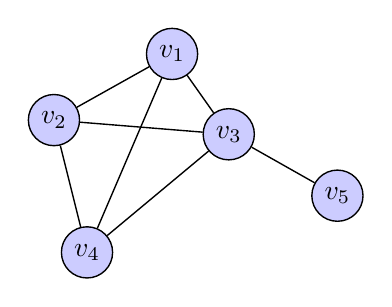
\begin{tikzpicture}[
  scale=0.6,
  vnode/.style={circle, fill=blue!20, draw=black, line width=0.5pt, inner sep=2pt, minimum size=6.5mm},
  edge/.style={line width=0.5pt, draw=black}
]

  % Posicionamiento de vértices asimétrico
  \node[vnode] (v1) at (0, 3.2) {$v_1$};
  \node[vnode] (v2) at (-2.5, 1.8) {$v_2$};
  \node[vnode] (v3) at (1.2, 1.5) {$v_3$};
  \node[vnode] (v4) at (-1.8, -1.0) {$v_4$};
  \node[vnode] (v5) at (3.5, 0.2) {$v_5$};

  % Aristas
  \draw[edge] (v1) -- (v2);
  \draw[edge] (v1) -- (v3);
  \draw[edge] (v2) -- (v4);
  \draw[edge] (v3) -- (v4);
  \draw[edge] (v3) -- (v5);
  \draw[edge] (v2) -- (v3);
  \draw[edge] (v1) -- (v4);

\end{tikzpicture}
} \vspace{6pt} \end{minipage} &
  \begin{minipage}{0.3\textwidth} \centering \vspace{8pt}
    $\begin{pmatrix}
      0 & 1 & 1 & 1 & 0 \\
      1 & 0 & 1 & 1 & 0 \\
      1 & 1 & 0 & 1 & 1 \\
      1 & 1 & 1 & 0 & 0 \\
      0 & 0 & 1 & 0 & 0
    \end{pmatrix}$
  \vspace{6pt} \end{minipage} \\
  \hline

  $G_2$ y $M_2$ &
  \begin{minipage}{0.3\textwidth} \centering \vspace{8pt} \resizebox{0.85\linewidth}{!}{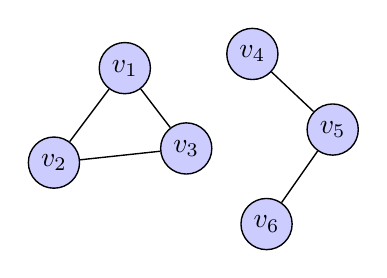
\begin{tikzpicture}[
  scale=0.6,
  vnode/.style={circle, fill=blue!20, draw=black, line width=0.5pt, inner sep=2pt, minimum size=6.5mm},
  edge/.style={line width=0.5pt, draw=black}
]

  % --- Componente 1 (Triángulo) ---
  \node[vnode] (v1) at (-2.5, 2.5) {$v_1$};
  \node[vnode] (v2) at (-4.0, 0.5) {$v_2$};
  \node[vnode] (v3) at (-1.2, 0.8) {$v_3$};

  \draw[edge] (v1) -- (v2) -- (v3) -- (v1);

  % --- Componente 2 (Camino/Trayectoria) ---
  \node[vnode] (v4) at (0.2, 2.8) {$v_4$};
  \node[vnode] (v5) at (1.9, 1.2) {$v_5$};
  \node[vnode] (v6) at (0.5, -0.8) {$v_6$};

  \draw[edge] (v4) -- (v5);
  \draw[edge] (v5) -- (v6);

\end{tikzpicture}
} \vspace{6pt} \end{minipage} &
  \begin{minipage}{0.3\textwidth} \centering \vspace{8pt}
    $\begin{pmatrix}
      0 & 1 & 1 & 0 & 0 & 0 \\
      1 & 0 & 1 & 0 & 0 & 0 \\
      1 & 1 & 0 & 0 & 0 & 0 \\
      0 & 0 & 0 & 0 & 1 & 0 \\
      0 & 0 & 0 & 1 & 0 & 1 \\
      0 & 0 & 0 & 0 & 1 & 0
    \end{pmatrix}$
  \vspace{6pt} \end{minipage} \\
  \hline

  $G_3$ y $M_3$ &
  \begin{minipage}{0.3\textwidth} \centering \vspace{8pt} \resizebox{0.85\linewidth}{!}{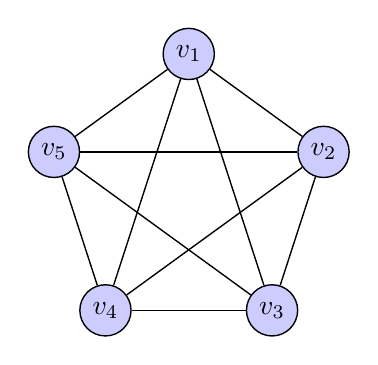
\begin{tikzpicture}[
  scale=1.0,
  vnode/.style={circle, fill=blue!20, draw=black, line width=0.5pt, inner sep=2pt, minimum size=6.5mm},
  edge/.style={line width=0.5pt, draw=black}
]

  % Vértices dispuestos en pentágono regular para máxima simetría
  \node[vnode] (v1) at (90:1.8) {$v_1$};
  \node[vnode] (v2) at (162:1.8) {$v_5$};
  \node[vnode] (v3) at (234:1.8) {$v_4$};
  \node[vnode] (v4) at (306:1.8) {$v_3$};
  \node[vnode] (v5) at (18:1.8) {$v_2$};

  % Todas las conexiones de un grafo completo K5 (10 aristas)
  \draw[edge] (v1) -- (v2);
  \draw[edge] (v1) -- (v3);
  \draw[edge] (v1) -- (v4);
  \draw[edge] (v1) -- (v5);

  \draw[edge] (v2) -- (v3);
  \draw[edge] (v2) -- (v4);
  \draw[edge] (v2) -- (v5);

  \draw[edge] (v3) -- (v4);
  \draw[edge] (v3) -- (v5);

  \draw[edge] (v4) -- (v5);

\end{tikzpicture}
} \vspace{6pt} \end{minipage} &
  \begin{minipage}{0.3\textwidth} \centering \vspace{8pt}
    $\begin{pmatrix}
      0 & 1 & 1 & 1 & 1 \\
      1 & 0 & 1 & 1 & 1 \\
      1 & 1 & 0 & 1 & 1 \\
      1 & 1 & 1 & 0 & 1 \\
      1 & 1 & 1 & 1 & 0
    \end{pmatrix}$
  \vspace{6pt} \end{minipage} \\
  \hline
\end{longtable}
\par\vspace{-0.3em}

\end{Ejm}
La ausencia de bucles en los grafos hace que todas las entradas en la diagonal principal de una matriz de adyacencia sean siempre $0$. Igualmente, el hecho de que en un grafo $G$ se tenga $v_iv_j\in E(G)$ si y sólo si $v_jv_i\in E(G)$, hace que cualquier matriz de adyacencia sea simétrica.\clearpage
\begin{Def}
   Sea $G$ un grafo. Dado un vértice $v\in V(G)$, denotamos por $\bm{A_v}$ al conjunto de todos los vértices adyacentes a $v$, es decir $A_v=\left\lbrace u\in V(G) \mid uv\in E(G)\right\rbrace$, y por $\bm{E_v}$ al conjunto de todas las aristas con las cuales es incidente $v$, es decir $E_v=\left\lbrace e\in E(G)\mid v\in e\right\rbrace$.
\end{Def}
De nuestra definicón de grafo se sigue inmediatamente que para cualquier par de vértices $u,v$ de un grafo, $u\in A_v$ si, y solo si, $v\in A_u$. En el grafo $G_2$ del \Cref{Ejm:cuatro_grafos}, tenemos que $A_{v_1}=\lbrace v_2,v_3,v_4\rbrace$, $A_{v_6}=\lbrace v_5\rbrace$, $E_{v_1}=\lbrace v_1v_2,v_1v_3,v_1v_4 \rbrace$ y $E_{v_6}=\lbrace v_5v_6\rbrace$. En el grafo $G_5$ del mismo ejemplo se tiene, para todo $i\in \left\lbrace 2,3,4,\dots\right\rbrace$, $A_{v_i}=\left\lbrace v_{i-1}, v_{i+1}\right\rbrace$ y $E_{v_i}=\left\lbrace v_{i-1}v_i, v_iv_{i+1}\right\rbrace$.\\
La siguiente proposición nos muestra el hecho natural de que la cantidad de vértices adyacentes a $v$ y la cantidad de aristas con las cuales es incidente $v$ es siempre la misma para, cualquier vértice $v$ en un grafo arbitrario.
\begin{Prop} \label{Prop:AvEv}
   En cualquier grafo $G$, dado $v\in V(G)$, se tiene $|A_v|=|E_v|$.
\end{Prop}
\begin{proof}
Definamos $f:A_v\to E_v: u\mapsto uv$. Nótese que si $u\in A_v$, entonces $uv\in E(G)$, y $v\in uv$, luego $uv\in E_v$, de modo que $f$ está bien definida. Se tiene que $f$ es inyectiva, pues si $u_1,u_2 \in A_v$ son tales que $f(u_1)=f(u_2)$ entonces $u_1v=u_2v$, es decir $\left\lbrace u_1,v\right\rbrace=\left\lbrace u_2,v\right\rbrace$, y como $u_1\neq v$ y $u_2\neq v$, entonces $u_1=u_2$. Además $f$ es sobreyectiva, pues dada $e\in E_v$, tenemos $v\in e$ y por tanto $e=uv$ para algún $u\in V(G)$; en particular $uv\in E(G)$, luego $u\in A_v$, y $f(u)=uv=e$. Por tanto $f$ es una biyección, con lo cual $|A_v|=|E_v|$.
\end{proof}
\begin{Def}
   Sea $G$ un grafo. El \textbf{grado} de un vértice $v\in V(G)$ se define como $d(v):=|A_v|$. Un vértice de grado $0$ se llama \textbf{aislado}, y uno de grado $1$ se llama una \textbf{hoja}.
\end{Def}
De este modo, el grado de un vértice se define como la cantidad de vértices adyacentes con él, que por la \Cref{Prop:AvEv}, es igual a la cantidad de aristas con las cuales es incidente. En el grafo $G_4$ del \Cref{Ejm:cuatro_grafos} se tiene $d(v_2)=3$ y $d(v_3)=4$, mientras que $v_1$ es un vértice aislado y $v_4$ es una hoja. En el grafo $G_5$ del mismo ejemplo se tiene $d(v_1)=1$ y $d(v_i)=2$ para todo $i\in \left\lbrace 2,3,4,\dots \right\rbrace$.
\begin{Def}
   Sea $G$ un grafo. Definimos el \textbf{grado mínimo} de $G$ como $\delta (G):= \min \left\lbrace d(v)\mid v\in V\right\rbrace$ y el \textbf{grado máximo} de $G$ como $\Delta (G):= \max \left\lbrace d(v)\mid v\in V\right\rbrace$, siempre que estos valores estén bien definidos.
\end{Def}
En el \Cref{Ejm:cuatro_grafos}, $\delta (G_1)=2=\Delta (G_1)$, $\delta (G_2)=1$, $\Delta (G_2)=3$, $\delta (G_3)=1$, $\Delta (G_3)=5$, $\delta (G_4)=0$, $\Delta (G_4)=4$, $\delta (G_5)=1$, $\Delta (G_5)=2$.
\begin{Def}
   Un grafo en el cual todos los vértices tienen el mismo grado $k$ se dice $\boldsymbol{k}$\textbf{-regular}, o simplemente \textbf{regular}.
\end{Def}
El grafo $G_1$ del \Cref{Ejm:cuatro_grafos} es $2$-regular. Naturalmente, en cualquier grafo $k$-regular $G$ se tiene $\delta(G)=\Delta(G)=k$.
\begin{Def}
   Un grafo se dice \textbf{localmente finito} si todos sus vértices tienen grado finito. 
\end{Def}
Todos los grafos finitos son localmente finitos. El grafo $G_5$ del \Cref{Ejm:cuatro_grafos} es un ejemplo de grafo infinito localmente finito. Se tienen otras situaciones, como se muestra a continuación.
\begin{Ejm}
   \phantom{o}
   \begin{figure}[H]
     \centering
       \resizebox{0.4\textwidth}{!}{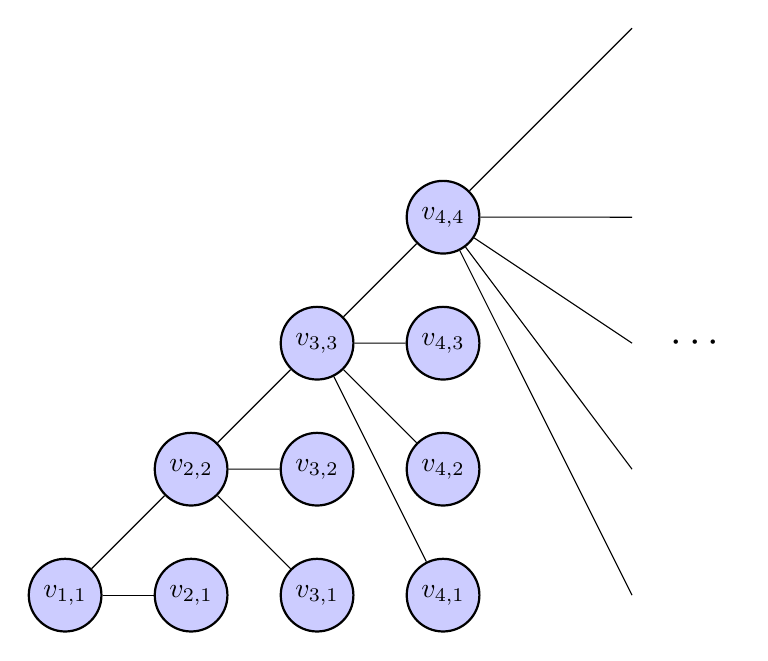
\begin{tikzpicture}
  [scale=.8,auto=left,every node/.style={circle,fill=blue!20,draw=black,thick}]
  \node (n1) at (0,0) {$v_{1,1}$};
  \node (n2) at (2,0)  {$v_{2,1}$};
  \node (n3) at (2,2)  {$v_{2,2}$};
  \node (n4) at (4,0) {$v_{3,1}$};
  \node (n5) at (4,2)  {$v_{3,2}$};
  \node (n6) at (4,4)  {$v_{3,3}$};
  \node (n7) at (6,0)  {$v_{4,1}$};
  \node (n8) at (6,2)  {$v_{4,2}$};
  \node (n9) at (6,4)  {$v_{4,3}$};
  \node (n10) at (6,6)  {$v_{4,4}$};

  \foreach \from/\to in {n1/n2,n1/n3, n3/n4, n3/n5, n3/n6, n6/n7, n6/n8, n6/n9, n6/n10}
    \draw (\from) -- (\to);

   \draw (n10) -- (9,0);
   \draw (n10) -- (9,2);
   \draw (n10) -- (9,4);
   \draw (n10) -- (9,6);
   \draw (n10) -- (9,9);
   
   %Etiqueta de puntos suspensivos
   \node[draw=none, fill=none, scale=1.5] at (10,4) {$\cdots$};
\end{tikzpicture}
} 
     \caption{Un grafo infinito localmente finito}
   \end{figure}
\end{Ejm}
\begin{Ejm}
   El siguiente grafo infinito no es localmente finito, pues $d(v_1)$ no es finito.
   \begin{figure}[H]
     \centering
       \resizebox{0.45\textwidth}{!}{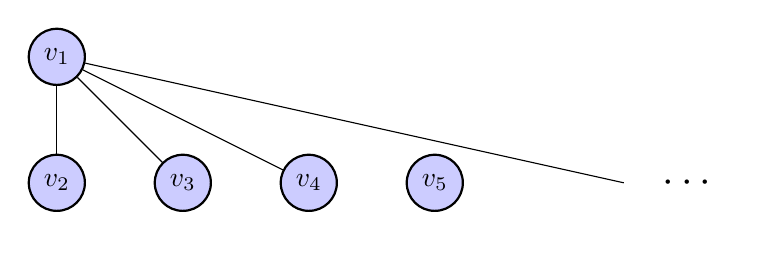
\begin{tikzpicture}
  [scale=.8,auto=left,every node/.style={circle,fill=blue!20,draw=black,thick}]
  \node (n1) at (0,2)  {$v_1$};
  \node (n2) at (0,0)  {$v_2$};
  \node (n3) at (2,0)  {$v_3$};
  \node (n4) at (4,0)  {$v_4$};
  \node (n5) at (6,0)  {$v_5$};


   \foreach \from/\to in {n1/n2,n1/n3, n1/n4}
      \draw (\from) -- (\to);
   
   \draw (n1) -- (9,0);

   \node[draw=none, fill=none, scale=1.5] at (10,0) {$\cdots$};
   
\end{tikzpicture}

} 
     \caption{Un grafo infinito que no es localmente finito}
   \end{figure}
\end{Ejm}
Un concepto importante en el presente trabajo es el de \textit{grafo conexo}. Para ello introducimos primero la definición de \textit{camino}.
\begin{Def}
   Un \textbf{camino} es un grafo no vacío $P=(V,E)$ de la forma
   $$
   V=\left\lbrace x_0, x_1, \dots, x_k\right\rbrace, \quad E=\left\lbrace x_0x_1, x_1x_2, \dots , x_{k-1}x_k\right\rbrace,
   $$
   para $k\in \mathbb{N}$, y donde todos los $x_i$, con $i\in \left\lbrace 0,1,\dots,k\right\rbrace$, son distintos. En este caso denotamos a $P$ mediante $x_0x_1\dots x_k$ o $x_kx_{k-1}\dots x_0$. Decimos que los vértices $x_0$ y $x_k$ están \textbf{conectados} por el camino P, y que $x_0$ y $x_k$ son los \textbf{extremos} de $P$. El número de aristas de un camino es su \textbf{longitud}. Denotamos por $\bm{P^k}$ a cualquier camino con $k$ vértices.
\end{Def}
\begin{Ejm}
   \phantom{o}
   \begin{itemize}
      \item $P^1$ es el grafo conformado por un solo vértice; es un camino de longitud $0$.
      \item Un camino de longitud $6$ es el siguiente:
      \begin{figure}[H]
        \centering
          \resizebox{0.3\textwidth}{!}{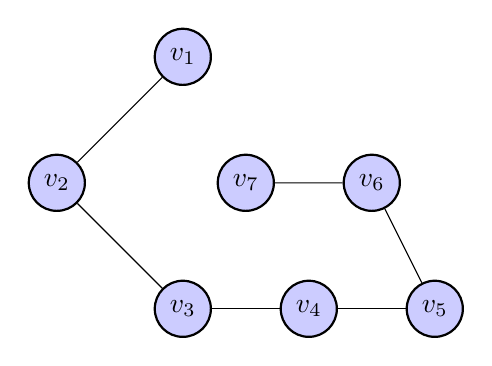
\begin{tikzpicture}
  [scale=.8,auto=left,every node/.style={circle,fill=blue!20,draw=black,thick}]
  \node (n1) at (2,4) {$v_1$};
  \node (n2) at (0,2)  {$v_2$};
  \node (n3) at (2,0)  {$v_3$};
  \node (n4) at (4,0) {$v_4$};
  \node (n5) at (6,0)  {$v_5$};
  \node (n6) at (5,2)  {$v_6$};
  \node (n7) at (3,2)  {$v_7$};

  \foreach \from/\to in {n1/n2,n2/n3, n3/n4, n4/n5, n5/n6, n6/n7}
    \draw (\from) -- (\to);
\end{tikzpicture}
}
        \caption{$P^7=v_1v_2v_3v_4v_5v_6v_7$}
      \end{figure}
   \end{itemize}
\end{Ejm}
\begin{Def}
   Sea $G$ un grafo. Decimos que dos vértices $u,v\in V(G)$ están \textbf{conectados por el camino $P$} en $G$ si $P\subseteq G$ y $P$ tiene a $u$ y $v$ como extremos.
\end{Def}
\begin{Ejm}
   \phantom{o}
   \begin{itemize}
      \item En el grafo $G_4$ del \Cref{Ejm:cuatro_grafos}, los vértices $v_6$ y $v_4$ están conectados, por ejemplo, por el camino $v_6v_2v_3v_4$, mientras que $v_1$ y $v_6$ no están conectados por un camino.
      \begin{figure}[H]
        \centering
          \resizebox{0.2\textwidth}{!}{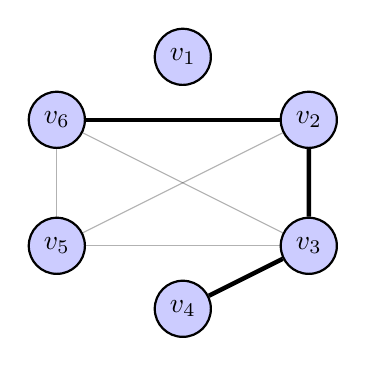
\begin{tikzpicture}
  [scale=.8,auto=left,every node/.style={circle,fill=blue!20,draw=black,thick}]
  \node (n1) at (2,4) {$v_1$};
  \node (n2) at (4,3)  {$v_2$};
  \node (n3) at (4,1)  {$v_3$};
  \node (n4) at (2,0) {$v_4$};
  \node (n5) at (0,1)  {$v_5$};
  \node (n6) at (0,3)  {$v_6$};

  \foreach \from/\to in {n3/n4,n2/n3, n2/n5, n2/n6, n3/n5, n3/n6, n5/n6}
  \draw[opacity=0.3] (\from) -- (\to);

  \foreach \from/\to in {n6/n2, n2/n3, n3/n4}
  \draw[ultra thick] (\from) -- (\to);

%\draw[ultra thick, red] (n2) -- (n6);
\end{tikzpicture}
}
        \caption{Un camino entre $v_6$ y $v_4$}
      \end{figure}
      \item En el grafo $G_1$ del \Cref{Ejm:Contenencia}, los vértices $v_4$ y $v_7$ están conectados por el camino $v_4v_5v_7$, pero $v_2$ y $v_6$ no están conectados por un camino.
      \begin{figure}[H]
        \centering
          \resizebox{0.3\textwidth}{!}{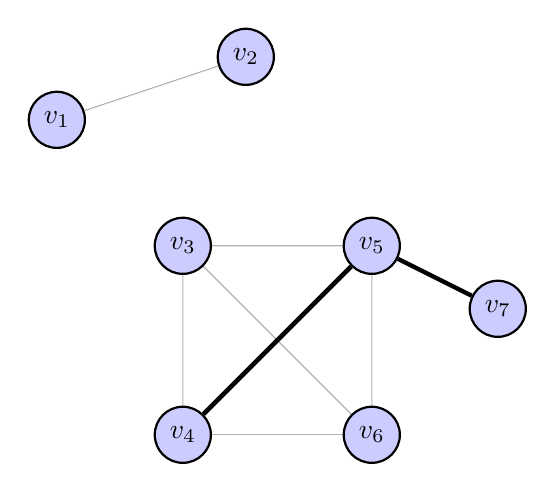
\begin{tikzpicture}
  [scale=.8,auto=left,every node/.style={circle,fill=blue!20,draw=black,thick}]
  \node (n1) at (0,5) {$v_1$};
  \node (n2) at (3,6) {$v_2$};
  \node (n3) at (2,3) {$v_3$};
  \node (n4) at (2,0) {$v_4$};
  \node (n5) at (5,3) {$v_5$};
  \node (n6) at (5,0) {$v_6$};
  \node (n7) at (7,2) {$v_7$};

  \foreach \from/\to in {n1/n2, n3/n5, n5/n6, n6/n4, n4/n3, n3/n6, n4/n5, n5/n7}
  \draw[opacity=0.3] (\from) -- (\to);


  \foreach \from/\to in {n4/n5, n5/n7}
  \draw[ultra thick] (\from) -- (\to);
\end{tikzpicture}
}
        \caption{Un camino entre $v_4$ y $v_7$}
      \end{figure}
   \end{itemize}
\end{Ejm}
\begin{Def}
   Un grafo $G$ es llamado \textbf{conexo} si $G\neq \emptyset$ y cualesquiera par de vértices  de $G$ están conectados por un camino en $G$. Si $G$ no es conexo, decimos que es \textbf{disconexo}. 
\end{Def}
Así, en el \Cref{Ejm:cuatro_grafos}, los grafos $G_1$, $G_3$ y $G_5$ son conexos, mientras que $G_2$ y $G_4$ son disconexos. Los grafos con un solo vértice son conexos.
\begin{Def}
   Sea $G$ un grafo. Un subgrafo conexo maximal de $G$ es llamado una \textbf{componente} de $G$. 
\end{Def}
Lo anterior nos quiere decir que un subgrafo $H\subseteq G$ es una componente de $G$ si y sólo si $H$ es conexo y además $H$ no está propiamente contenido en otro subgrafo conexo de $G$. Naturalmente, un grafo es conexo si y sólo si tiene una única componente. Además, como los grafos conexos son no vacíos, se sigue que el grafo vacío no tiene componentes.
\begin{Ejm}
   En los siguientes grafos se encierra con una línea punteada cada una de sus componentes.
   \begin{figure}[H]
     \centering
       \resizebox{0.45\textwidth}{!}{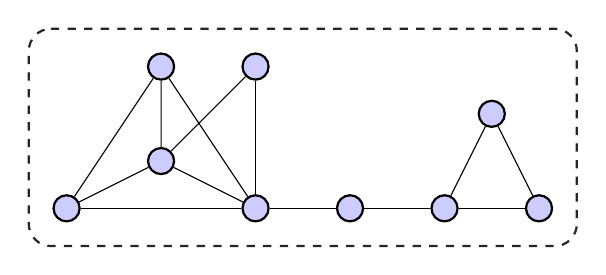
\begin{tikzpicture}[scale=.6,auto=left,every node/.style={circle,fill=blue!20,draw=black,thick}]
  \node (n1) at (0,0) {};
  \node (n2) at (2,3) {};
  \node (n3) at (2,1) {};
  \node (n4) at (4,3) {};
  \node (n5) at (4,0) {};
  \node (n6) at (6,0) {};
  \node (n7) at (8,0) {};
  \node (n8) at (9,2) {};
  \node (n9) at (10,0) {};
  
  \foreach \from/\to in {n1/n2,n1/n3,n1/n5,n2/n3,n2/n5,n3/n4,n3/n5,n4/n5,n5/n6,n6/n7,n7/n8,n7/n9,n8/n9}
    \draw (\from) -- (\to);

  % --- Envolvente estilo mano alzada para la componente conexa ---
  \begin{scope}[
    dashed,
    black!85,
    thick,
    decorate,
    decoration={random steps, segment length=5mm, amplitude=1.2mm}
  ]
    \draw[rounded corners=8pt] 
      (-0.8,3.8) -- (10.8,3.8) -- (10.8,-0.8) -- (-0.8,-0.8) -- cycle;
  \end{scope}

\end{tikzpicture}
}
     \caption{Un grafo con una componente}
   \end{figure}
   \begin{figure}[H]
     \centering
       \resizebox{0.35\textwidth}{!}{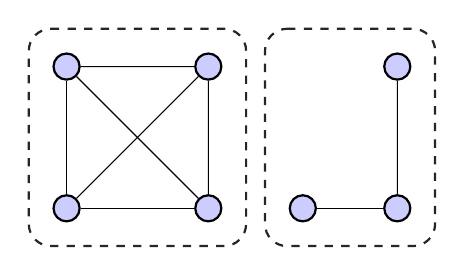
\begin{tikzpicture}
[scale=.6,auto=left,every node/.style={circle,fill=blue!20,draw=black,thick}]

  % Componente izquierda (Grafo completo K_4)
  \node (n1) at (0,3) {};
  \node (n2) at (3,3) {};
  \node (n3) at (0,0) {};
  \node (n4) at (3,0) {};

  \foreach \from/\to in {n1/n2,n1/n3,n1/n4,n2/n3,n2/n4,n3/n4}
    \draw (\from) -- (\to);

  % Componente derecha (Camino P_3)
  \node (n5) at (5,0) {};
  \node (n6) at (7,0) {};
  \node (n7) at (7,3) {};

  \foreach \from/\to in {n5/n6,n6/n7}
    \draw (\from) -- (\to);

  % --- Envolventes estilo mano alzada rectangulares ---
  \begin{scope}[
    dashed,
    black!85,
    thick,
    decorate,
    decoration={random steps, segment length=5mm, amplitude=1.2mm}
  ]
    % Envolvente izquierda (K_4)
    \draw[rounded corners=8pt] 
      (-0.8,3.8) -- (3.8,3.8) -- (3.8,-0.8) -- (-0.8,-0.8) -- cycle;

    % Envolvente derecha (P_3)
    \draw[rounded corners=8pt] 
      (4.2,3.8) -- (7.8,3.8) -- (7.8,-0.8) -- (4.2,-0.8) -- cycle;
  \end{scope}

\end{tikzpicture}
}
     \caption{Un grafo con dos componentes}
   \end{figure}
   \begin{figure}[H]
     \centering
       \resizebox{0.55\textwidth}{!}{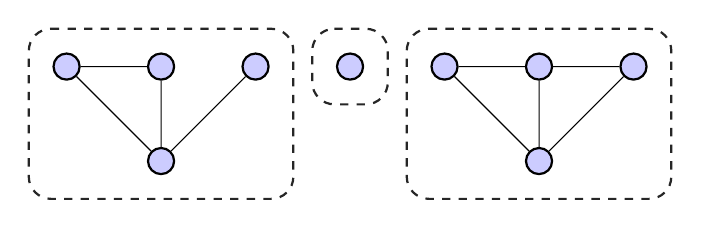
\begin{tikzpicture}
[scale=.6,auto=left,every node/.style={circle,fill=blue!20,draw=black,thick}]

  % Componente izquierda
  \node (n1) at (0,2) {};
  \node (n2) at (2,2) {};
  \node (n3) at (2,0) {};
  \node (n4) at (4,2) {};

  \foreach \from/\to in {n1/n2,n1/n3,n2/n3,n3/n4}
    \draw (\from) -- (\to);

  % Vértice aislado central
  \node (n5) at (6,2) {};

  % Componente derecha
  \node (n6) at (8,2) {};
  \node (n7) at (10,2) {};
  \node (n8) at (10,0) {};
  \node (n9) at (12,2) {};

  \foreach \from/\to in {n6/n7,n6/n8,n7/n8,n7/n9,n8/n9}
    \draw (\from) -- (\to);

  % --- Envolventes estilo mano alzada rectangulares ---
  \begin{scope}[
    dashed,
    black!85, % Color más oscuro
    thick,
    decorate,
    decoration={random steps, segment length=5mm, amplitude=1.2mm}
  ]
    % Envolvente izquierda (cuadrada/rectangular)
    \draw[rounded corners=8pt] 
      (-0.8,2.8) -- (4.8,2.8) -- (4.8,-0.8) -- (-0.8,-0.8) -- cycle;

    % Envolvente centro (alrededor de n5)
    \draw[rounded corners=8pt] 
      (5.2,2.8) -- (6.8,2.8) -- (6.8,1.2) -- (5.2,1.2) -- cycle;

    % Envolvente derecha (cuadrada/rectangular)
    \draw[rounded corners=8pt] 
      (7.2,2.8) -- (12.8,2.8) -- (12.8,-0.8) -- (7.2,-0.8) -- cycle;
  \end{scope}

\end{tikzpicture}
}
     \caption{Un grafo con tres componentes}
   \end{figure}
\end{Ejm}
Dado un grafo, se puede inducir un nuevo grafo al eliminar adecuadamente un subconjunto de vértices.
\begin{Def}
   Sean $G$ un grafo y $S\subseteq V(G)$. Denotamos por $\bm{G-S}$ al subgrafo de $G$ inducido por $V(G)\setminus S$, es decir, $G-S=G[V(G)\setminus S]$. 
\end{Def}\clearpage
\begin{Ejm}\label{Ejm:Supresion}
   \phantom{0}
   \begin{itemize}
      \item Si $S=\left\lbrace v_3,v_4\right\rbrace$ entonces:  
         \begin{figure}[H]
  \centering
  \resizebox{0.2\textwidth}{!}{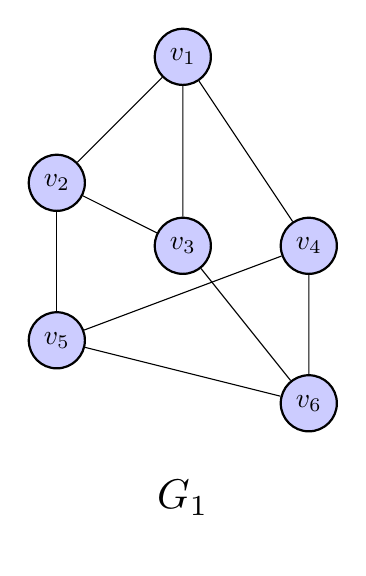
\begin{tikzpicture}
  [scale=.8,auto=left,every node/.style={circle,fill=blue!20,draw=black,thick}]
  \node (n1) at (3,6) {$v_1$};
  \node (n2) at (1,4) {$v_2$};
  \node (n3) at (3,3) {$v_3$};
  \node (n4) at (5,3) {$v_4$};
  \node (n5) at (1,1.5) {$v_5$};
  \node (n6) at (5,0.5) {$v_6$};

  \foreach \from/\to in {n1/n2, n1/n3, n1/n4, n2/n3, n2/n5, n3/n6, n4/n5, n4/n6, n5/n6}
    \draw (\from) -- (\to);

   \node[draw=none, fill=none, scale=1.5] at (3,-1) {$G_1$};
\end{tikzpicture}
} \hspace{2cm}
  \resizebox{0.2\textwidth}{!}{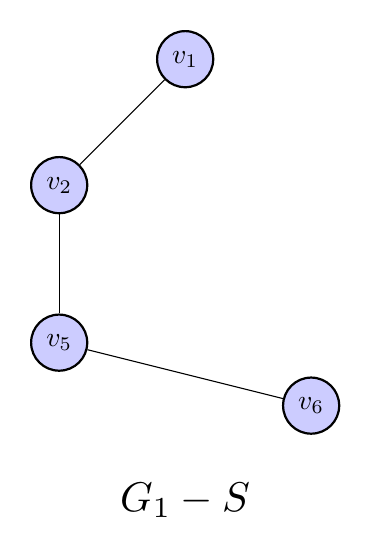
\begin{tikzpicture}
  [scale=.8,auto=left,every node/.style={circle,fill=blue!20,draw=black,thick}]
\useasboundingbox (0.5,-1.5) rectangle (5.5,6.5);
  \node (n1) at (3,6) {$v_1$};
  \node (n2) at (1,4) {$v_2$};
  \node (n3) at (3,3) [opacity=0]{$v_3$};
  \node (n4) at (5,3) [opacity=0]{$v_4$};
  \node (n5) at (1,1.5) {$v_5$};
  \node (n6) at (5,0.5) {$v_6$};

  \foreach \from/\to in {n1/n2, n2/n5, n5/n6}
    \draw (\from) -- (\to);

   \node[draw=none, fill=none, scale=1.5] at (3,-1) {$G_1-S$};
\end{tikzpicture}
} 
    \caption{$G_1$ y $G_1-S$}
\end{figure}
  
      \item Si $S'=\left\lbrace v_2,v_3,v_5\right\rbrace$ entonces:
         \vspace{1em}
         \par\vspace*{-5em}
{\centering
  \resizebox{0.23\textwidth}{!}{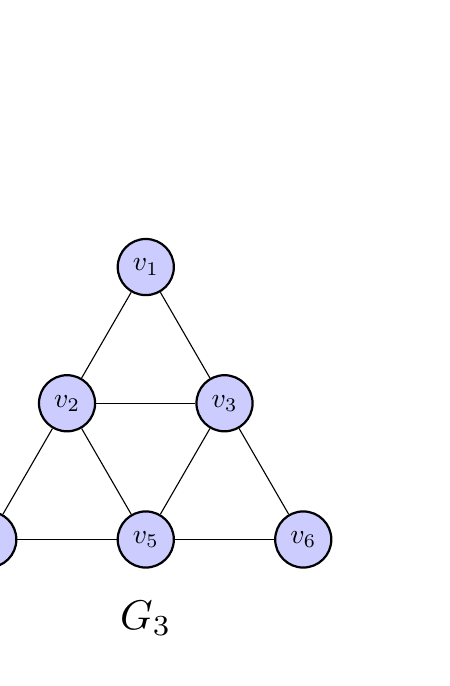
\begin{tikzpicture}
  [scale=1,auto=left,every node/.style={circle,fill=blue!20,draw=black,thick}]
\useasboundingbox (0.5,-1.5) rectangle (5.5,6.5);
  % Posiciones simétricas en forma de triángulo equilátero
  \node (n1) at (2,3.46) {$v_1$};
  \node (n2) at (1,1.73) {$v_2$};
  \node (n3) at (3,1.73) {$v_3$};
  \node (n4) at (0,0)    {$v_4$};
  \node (n5) at (2,0)    {$v_5$};
  \node (n6) at (4,0)    {$v_6$};

  % Aristas del grafo base (malla triangular)
  \foreach \from/\to in {n1/n2, n1/n3, n2/n3, n2/n4, n2/n5, n3/n5, n3/n6, n4/n5, n5/n6}
    \draw (\from) -- (\to);

   \node[draw=none, fill=none, scale=1.5] at (2,-1) {$G_3$};
\end{tikzpicture}
}%
  \hspace{2cm}%
  \resizebox{0.23\textwidth}{!}{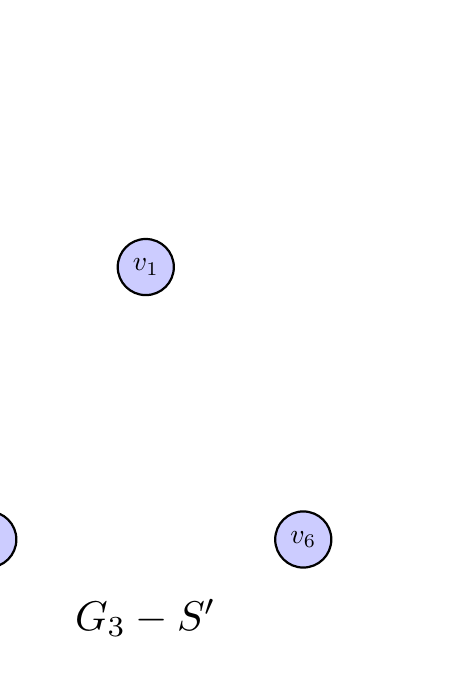
\begin{tikzpicture}
  [scale=1,auto=left,every node/.style={circle,fill=blue!20,draw=black,thick}]
\useasboundingbox (0.5,-1.5) rectangle (5.5,6.5); 
% Posiciones simétricas en forma de triángulo equilátero
  \node (n1) at (2,3.46) {$v_1$};
  \node (n2) at (1,1.73) [opacity=0]{$v_2$};
  \node (n3) at (3,1.73) [opacity=0]{$v_3$};
  \node (n4) at (0,0)    {$v_4$};
  \node (n5) at (2,0)    [opacity=0]{$v_5$};
  \node (n6) at (4,0)    {$v_6$};

  % Aristas del grafo base (malla triangular)
  %\foreach \from/\to in {n1/n2, n1/n3, n2/n3, n2/n4, n2/n5, n3/n5, n3/n6, n4/n5, n5/n6}
   % \draw (\from) -- (\to);

   \node[draw=none, fill=none, scale=1.5] at (2,-1) {$G_3-S'$};
\end{tikzpicture}
}\par
  \vspace{0.3em}%
  \captionof{figure}{$G_3$ y $G_3-S'$}
\par}
\vspace{1em}
  
   \end{itemize}
\end{Ejm}
Como se ve con el grafo $G_3$ del \Cref{Ejm:Supresion}, la supresión de algunos vértices en un grafo puede aumentar su número de componentes. La siguiente definición trata de casos especiales donde se da esta situación.
\begin{Def}
   Sea $G$ un grafo. Decimos que $v\in V(G)$ es un \textbf{vértice de corte} de $G$ si $G-\left\lbrace v\right\rbrace$ tiene más componentes que $G$. Si $G$ es conexo, decimos que un subconjunto de vértices $C\subseteq V(G)$ es un \textbf{conjunto de corte} de $G$ si $G-C$ tiene más de una componente. Si además, ningún subconjunto propio de $C$ es un conjunto de corte de $G$, decimos que $C$ es un \textbf{conjunto de corte minimal} de $G$.  
\end{Def}
\begin{Ejm}
   \phantom{o}
   \begin{itemize}
      \item En el grafo $G_1$, $v_1$ es un vértice de corte, pues $G_1-\left\lbrace v_1\right\rbrace$ tiene cuatro componentes, mientras que $G_1$ tiene dos componentes.
         \begin{figure}[H]
  \centering
  \resizebox{0.35\textwidth}{!}{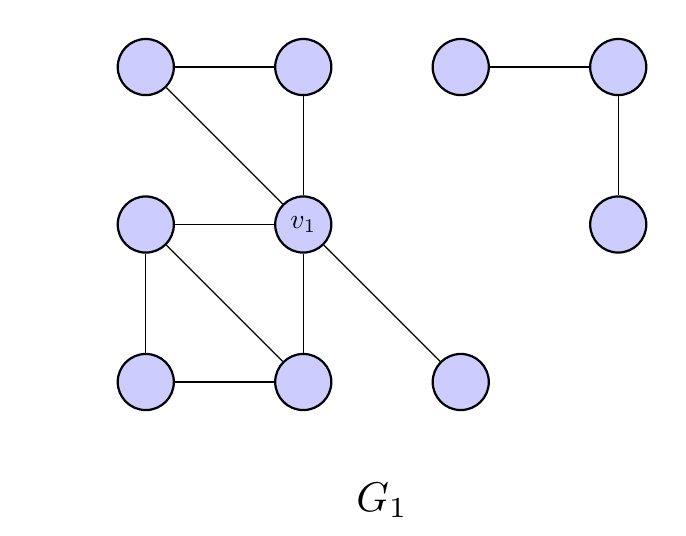
\begin{tikzpicture}[scale=1, auto=left, every node/.style={circle, fill=blue!20, draw=black, thick}]
    \node (v) at (3,2) {$v_1$};

  % Componente superior izquierda
    \node (u1) at (1,4) {\phantom{$v_1$}};
  \node (u2) at (3,4) {\phantom{$v_1$}};

  % Componente inferior izquierda
  \node (w1) at (1,2) {\phantom{$v_1$}};
  \node (w2) at (1,0) {\phantom{$v_1$}};
  \node (w3) at (3,0) {\phantom{$v_1$}};

  % Hoja inferior derecha
  \node (x1) at (5,0) {\phantom{$v_1$}};

  % Componente disjunta superior derecha
  \node (y1) at (5,4) {\phantom{$v_1$}};
  \node (y2) at (7,4) {\phantom{$v_1$}};
  \node (y3) at (7,2) {\phantom{$v_1$}};

  % Aristas
  \draw (u1) -- (u2);
  \draw (u1) -- (v);
  \draw (u2) -- (v);

  \draw (w1) -- (w2);
  \draw (w2) -- (w3);
  \draw (w1) -- (w3);
  \draw (w1) -- (v);
  \draw (w3) -- (v);

  \draw (v) -- (x1);

  \draw (y1) -- (y2);
  \draw (y2) -- (y3);

% Forzar Bounding Box idéntico en ambos diagramas
  \useasboundingbox (-0.5,-1.6) rectangle (7.5,4.5);
  % Etiqueta del grafo
  \node[draw=none, fill=none, scale=1.5] at (4,-1.5) {$G_1$};
\end{tikzpicture}
} \hspace{2cm}
  \resizebox{0.35\textwidth}{!}{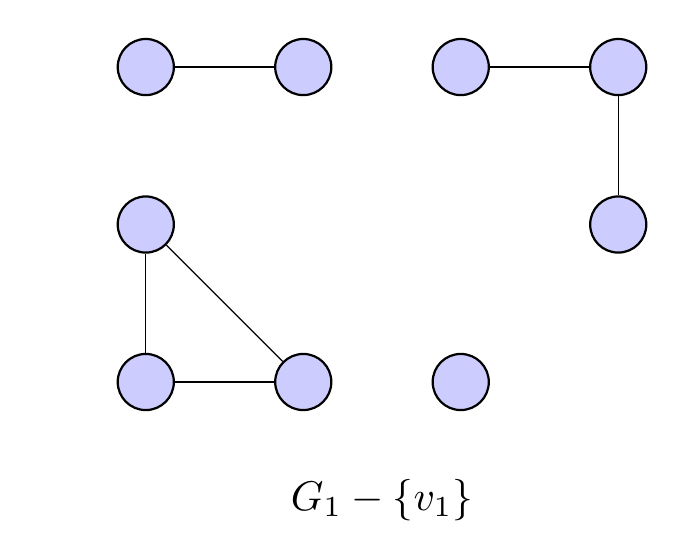
\begin{tikzpicture}[scale=1, auto=left, every node/.style={circle, fill=blue!20, draw=black, thick}]
  \node (v) at (3,2) [opacity=0]{$v_1$};

  % Componente superior izquierda
  \node (u1) at (1,4) {\phantom{$v_1$}};
  \node (u2) at (3,4) {\phantom{$v_1$}};

  % Componente inferior izquierda
  \node (w1) at (1,2) {\phantom{$v_1$}};
  \node (w2) at (1,0) {\phantom{$v_1$}};
  \node (w3) at (3,0) {\phantom{$v_1$}};

  % Hoja inferior derecha
  \node (x1) at (5,0) {\phantom{$v_1$}};

  % Componente disjunta superior derecha
  \node (y1) at (5,4) {\phantom{$v_1$}};
  \node (y2) at (7,4) {\phantom{$v_1$}};
  \node (y3) at (7,2) {\phantom{$v_1$}};

  % Aristas
  \draw (u1) -- (u2);

  \draw (w1) -- (w2);
  \draw (w2) -- (w3);
  \draw (w1) -- (w3);

  \draw (y1) -- (y2);
  \draw (y2) -- (y3);

% Forzar Bounding Box idéntico en ambos diagramas
  \useasboundingbox (-0.5,-1.6) rectangle (7.5,4.5);
  % Etiqueta del grafo
  \node[draw=none, fill=none, scale=1.5] at (4,-1.5) {$G_1-\left\lbrace v_1\right\rbrace$};
\end{tikzpicture}
} 
  \caption{Un vértice de corte}
\end{figure}
\vspace{-0.5cm}
      %\item En la siguiente figura, se tiene que $S:=\{u,v,w\}$ es un conjunto de corte del grafo conexo $G_2$, pues $G_2-S$ tiene dos componentes.\vspace{0.1cm}
      \item Tomemos $S=\{u,v,w\}$ y $S'=\{u,v\}$. En el grafo conexo $G_2$ que se muestra en la siguiente figura, $S$ es un conjunto de corte, pues $G_2-S$ tiene dos componentes.\vspace{0.1cm}
      \begin{figure}[H]
        \centering
        \resizebox{0.3\textwidth}{!}{\definecolor{customred}{HTML}{E7180B}

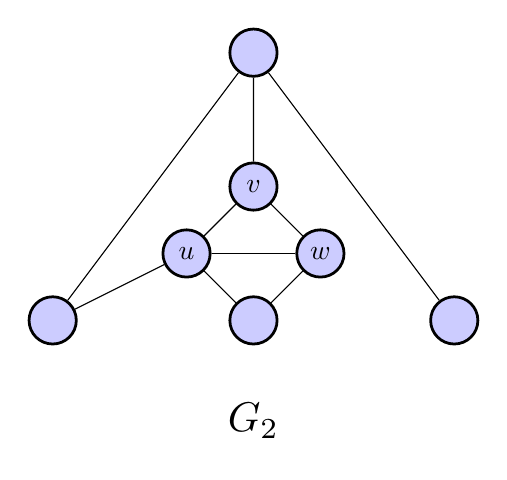
\begin{tikzpicture}[scale=0.85, auto=left]
  \tikzset{
    blue_node/.style={circle, fill=blue!20, draw, line width=1pt, inner sep=2pt, minimum size=6mm},
    red_node/.style={circle, fill=customred!20, draw=customred, line width=1pt, inner sep=2pt, minimum size=6mm}
  }

  % Vértices según la cuadrícula
  % Vértices con etiqueta
  \node[blue_node] (v) at (3,2) {$v$};
  \node[blue_node] (u) at (2,1) {$u$};
  \node[blue_node] (w) at (4,1) {$w$};

  % Vértices sin etiqueta (círculos vacíos)
  \node[blue_node] (top) at (3,4) {};
  \node[blue_node] (bottom) at (3,0) {};
  \node[blue_node] (left_bottom) at (0,0) {};
  \node[blue_node] (right_bottom) at (6,0) {};

  % Aristas del diamante interno (u, v, w, bottom)
  \draw (v) -- (u);
  \draw (v) -- (w);
  \draw (u) -- (w);
  \draw (u) -- (bottom);
  \draw (w) -- (bottom);

  % Conexiones del vértice superior (top)
  \draw (top) -- (v);
  \draw (top) -- (left_bottom);
  \draw (top) -- (right_bottom);

  % Conexión del vértice inferior izquierdo
  \draw (left_bottom) -- (u);

  % Bounding box para asegurar la alineación de la figura
  %\useasboundingbox (-0.5,-1.6) rectangle (6.5,6.5);

  % Etiqueta del grafo
  \node[draw=none, fill=none, scale=1.5] at (3,-1.5) {$G_2$};
\end{tikzpicture}
}\hspace{2cm}
        \resizebox{0.3\textwidth}{!}{\definecolor{customred}{HTML}{E7180B}

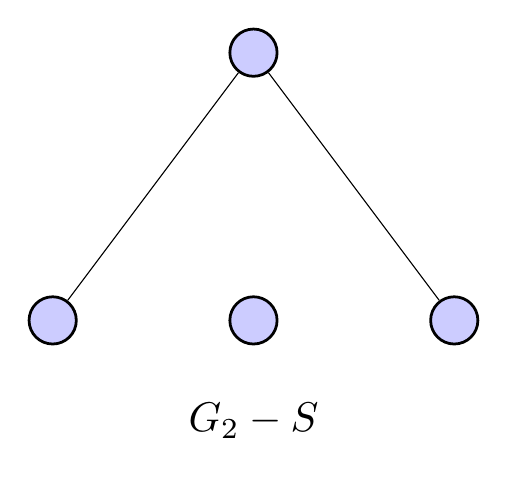
\begin{tikzpicture}[scale=0.85, auto=left]
  \tikzset{
    blue_node/.style={circle, fill=blue!20, draw, line width=1pt, inner sep=2pt, minimum size=6mm},
    red_node/.style={circle, fill=customred!20, draw=customred, line width=1pt, inner sep=2pt, minimum size=6mm}
  }

  % Vértices según la cuadrícula
  % Vértices con etiqueta
  \node[blue_node] (v) at (3,2) [opacity=0]{$v$};
  \node[blue_node] (u) at (2,1) [opacity=0]{$u$};
  \node[blue_node] (w) at (4,1) [opacity=0]{$w$};

  % Vértices sin etiqueta (círculos vacíos)
  \node[blue_node] (top) at (3,4) {};
  \node[blue_node] (bottom) at (3,0) {};
  \node[blue_node] (left_bottom) at (0,0) {};
  \node[blue_node] (right_bottom) at (6,0) {};

  % Aristas del diamante interno (u, v, w, bottom)

  % Conexiones del vértice superior (top)
  \draw (top) -- (left_bottom);
  \draw (top) -- (right_bottom);

  % Conexión del vértice inferior izquierdo

  % Bounding box para asegurar la alineación de la figura
  %\useasboundingbox (-0.5,-1.6) rectangle (6.5,6.5);

  % Etiqueta del grafo
  \node[draw=none, fill=none, scale=1.5] at (3,-1.5) {$G_2-S$};
\end{tikzpicture}
}
        \caption{$S$ es un conjunto de corte de $G_2$}
     \end{figure}\vspace{-0.4cm}
      Sin embargo $S$ no es un conjunto de corte minimal de $G_2$, ya que $S'\subsetneq S$ y $S'$ es un conjunto de corte de $G_2$, pues $G_2-S'$ tiene dos componentes.
      \begin{figure}[H]
        \centering
          \resizebox{0.3\textwidth}{!}{\definecolor{customred}{HTML}{E7180B}

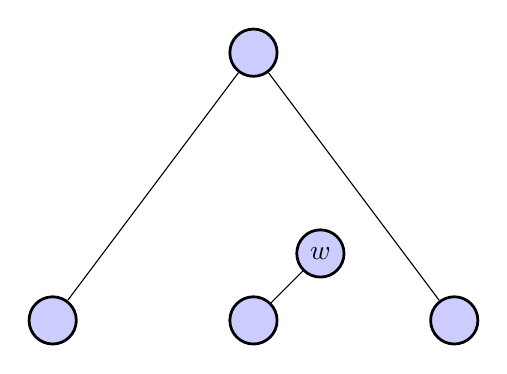
\begin{tikzpicture}[scale=0.85, auto=left]
  \tikzset{
    blue_node/.style={circle, fill=blue!20, draw, line width=1pt, inner sep=2pt, minimum size=6mm},
    red_node/.style={circle, fill=customred!20, draw=customred, line width=1pt, inner sep=2pt, minimum size=6mm}
  }

  % Vértices según la cuadrícula
  % Vértices con etiqueta
  \node[blue_node] (v) at (3,2) [opacity=0]{$v$};
  \node[blue_node] (u) at (2,1) [opacity=0]{$u$};
  \node[blue_node] (w) at (4,1) {$w$};

  % Vértices sin etiqueta (círculos vacíos)
  \node[blue_node] (top) at (3,4) {};
  \node[blue_node] (bottom) at (3,0) {};
  \node[blue_node] (left_bottom) at (0,0) {};
  \node[blue_node] (right_bottom) at (6,0) {};

  % Aristas del diamante interno (u, v, w, bottom)

  % Conexiones del vértice superior (top)
  \draw (top) -- (left_bottom);
  \draw (top) -- (right_bottom);
  \draw (w) -- (bottom);
  % Conexión del vértice inferior izquierdo

  % Bounding box para asegurar la alineación de la figura
  %\useasboundingbox (-0.5,-1.6) rectangle (6.5,6.5);

  % Etiqueta del grafo
  %\node[draw=none, fill=none, scale=1.5] at (3,-1.5) {$G_2-S'$};
\end{tikzpicture}
}
        \caption{El grafo $G_2-S'$}
      \end{figure}
      En cambio se tiene que $S'$ sí es un conjunto de corte minimal de $G_2$, pues ni $\{u\}$ ni $\{v\}$ son conjuntos de corte de $G_2$, ya que $G_2-\{u\}$ y $G_2-\{v\}$ son grafos conexos.\vspace{-1.2cm}
      \begin{figure}[H]
        \centering
           \resizebox{0.3\textwidth}{!}{\definecolor{customred}{HTML}{E7180B}

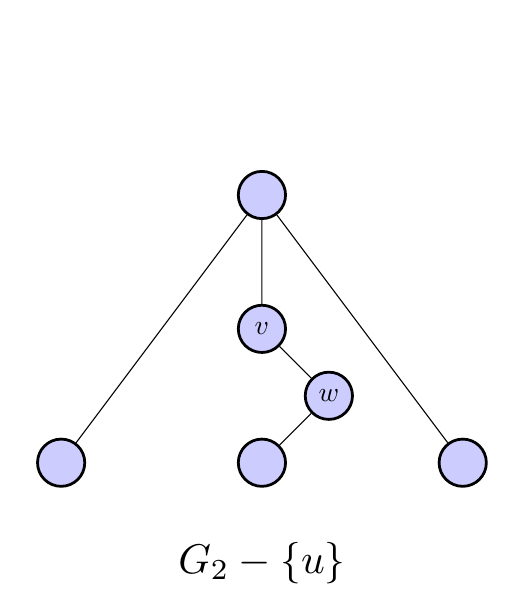
\begin{tikzpicture}[scale=0.85, auto=left]
  \tikzset{
    blue_node/.style={circle, fill=blue!20, draw, line width=1pt, inner sep=2pt, minimum size=6mm},
    red_node/.style={circle, fill=customred!20, draw=customred, line width=1pt, inner sep=2pt, minimum size=6mm}
  }

  % Vértices según la cuadrícula
  % Vértices con etiqueta
  \node[blue_node] (v) at (3,2) {$v$};
  \node[blue_node] (u) at (2,1) [opacity=0]{$u$};
  \node[blue_node] (w) at (4,1) {$w$};

  % Vértices sin etiqueta (círculos vacíos)
  \node[blue_node] (top) at (3,4) {};
  \node[blue_node] (bottom) at (3,0) {};
  \node[blue_node] (left_bottom) at (0,0) {};
  \node[blue_node] (right_bottom) at (6,0) {};

  % Aristas del diamante interno (u, v, w, bottom)
  \draw (v) -- (w);
  \draw (w) -- (bottom);

  % Conexiones del vértice superior (top)
  \draw (top) -- (v);
  \draw (top) -- (left_bottom);
  \draw (top) -- (right_bottom);

  % Conexión del vértice inferior izquierdo

  % Bounding box para asegurar la alineación de la figura
  \useasboundingbox (-0.5,-1.6) rectangle (6.5,6.5);

  % Etiqueta del grafo
  \node[draw=none, fill=none, scale=1.5] at (3,-1.5) {$G_2-\left\lbrace u\right\rbrace$};
\end{tikzpicture}
}\hspace{2cm}
          \resizebox{0.3\textwidth}{!}{\definecolor{customred}{HTML}{E7180B}

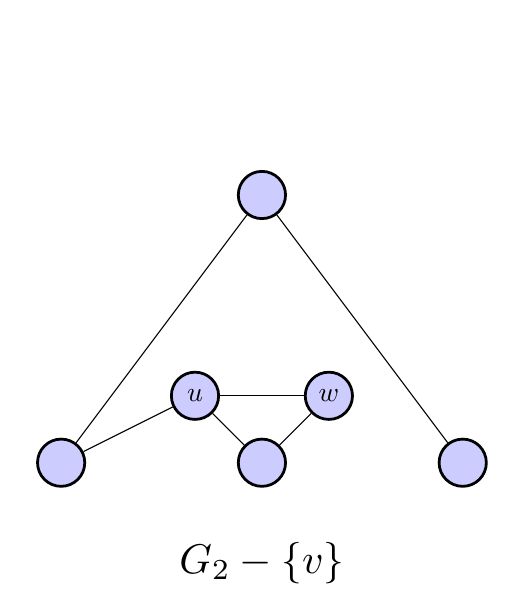
\begin{tikzpicture}[scale=0.85, auto=left]
  \tikzset{
    blue_node/.style={circle, fill=blue!20, draw, line width=1pt, inner sep=2pt, minimum size=6mm},
    red_node/.style={circle, fill=customred!20, draw=customred, line width=1pt, inner sep=2pt, minimum size=6mm}
  }

  % Vértices según la cuadrícula
  % Vértices con etiqueta
  \node[blue_node] (v) at (3,2) [opacity=0]{$v$};
  \node[blue_node] (u) at (2,1) {$u$};
  \node[blue_node] (w) at (4,1) {$w$};

  % Vértices sin etiqueta (círculos vacíos)
  \node[blue_node] (top) at (3,4) {};
  \node[blue_node] (bottom) at (3,0) {};
  \node[blue_node] (left_bottom) at (0,0) {};
  \node[blue_node] (right_bottom) at (6,0) {};

  % Aristas del diamante interno (u, v, w, bottom)
  \draw (u) -- (w);
  \draw (u) -- (bottom);
  \draw (w) -- (bottom);

  % Conexiones del vértice superior (top)
  \draw (top) -- (left_bottom);
  \draw (top) -- (right_bottom);

  % Conexión del vértice inferior izquierdo
  \draw (left_bottom) -- (u);

  % Bounding box para asegurar la alineación de la figura
  \useasboundingbox (-0.5,-1.6) rectangle (6.5,6.5);

  % Etiqueta del grafo
  \node[draw=none, fill=none, scale=1.5] at (3,-1.5) {$G_2-\left\lbrace v\right\rbrace$};
\end{tikzpicture}
}
          \vspace{0.5cm}
        \caption{Los grafos $G_2-\{u\}$ y $G_2-\{v\}$ son conexos}
      \end{figure}
   \end{itemize}
\end{Ejm}
\begin{Def}
   Sean $G$ un grafo y $S\subseteq V(G)$. Decimos que $S$ es \textbf{independiente} si para cualesquiera $u,v\in S$ se tiene $uv\notin E(G)$. En cambio, decimos que $S$ es un \textbf{clique} si para cualesquiera $u,v\in S$ se tiene $uv\in E(G)$.
\end{Def}
De esta forma, un subconjunto de vértices de un grafo es independiente si ningún par de estos vértices son adyacentes, y es un clique si cualquier par de estos vértices son adyacentes. En el \Cref{Ejm:cuatro_grafos}, $\left\lbrace v_2,v_4,v_6\right\rbrace$ es un conjunto independiente de $G_1$, $\left\lbrace v_1,v_2,v_3,v_4\right\rbrace$ es un clique de $G_2$, $\left\lbrace v_2,v_3,v_4,v_5,v_6\right\rbrace$ es un conjunto independiente de $G_3$ y $\left\lbrace v_2,v_3,v_5,v_6\right\rbrace$ es un clique de $G_4$.
\begin{Def}
   Dado un grafo $G=(V,E)$, su \textbf{complemento}, denotado $\overline{G}$, es el grafo con conjunto de vértices $V$ y conjunto de aristas $[V]^2\setminus E$. 
\end{Def}
Así, $\overline{G}$ mantiene los vértices de $G$, pero dos vértice son adyacentes en $\overline{G}$ si y sólo si no son adyacentes en $G$.
\begin{Ejm}
   La siguiente figura muestra ejemplos de grafos y sus complementos.\clearpage
   \par\vspace{1.5em}
{\centering
 % Fila superior (Diag33 y Diag34)
 \makebox[0.3\textwidth]{\resizebox{0.2\textwidth}{!}{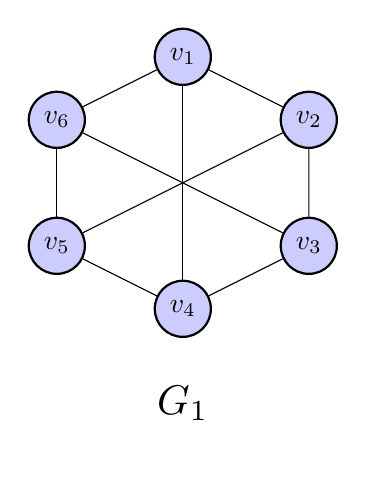
\begin{tikzpicture}
  [scale=.8,auto=left,every node/.style={circle,fill=blue!20,draw=black,thick}]
  \node (n1) at (2,4) {$v_1$};
  \node (n2) at (4,3)  {$v_2$};
  \node (n3) at (4,1)  {$v_3$};
  \node (n4) at (2,0) {$v_4$};
  \node (n5) at (0,1)  {$v_5$};
  \node (n6) at (0,3)  {$v_6$};

  \foreach \from/\to in {n1/n2,n2/n3,n3/n4,n4/n5,n5/n6,n6/n1,n6/n3,n1/n4,n2/n5}
    \draw (\from) -- (\to);

  % Etiqueta G_1 debajo del grafo
  \node[draw=none, fill=none, scale=1.5] at (2,-1.5) {$G_1$};

\end{tikzpicture}
}}%
 \hspace{2cm}%
 \makebox[0.3\textwidth]{\resizebox{0.2\textwidth}{!}{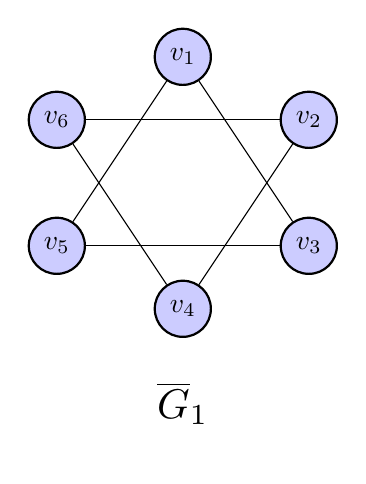
\begin{tikzpicture}
  [scale=.8,auto=left,every node/.style={circle,fill=blue!20,draw=black,thick}]
  \node (n1) at (2,4) {$v_1$};
  \node (n2) at (4,3) {$v_2$};
  \node (n3) at (4,1) {$v_3$};
  \node (n4) at (2,0) {$v_4$};
  \node (n5) at (0,1) {$v_5$};
  \node (n6) at (0,3) {$v_6$};

  % Aristas del complemento \overline{G}_1
  % Aristas rectas
  \draw (n1) -- (n3);
  \draw (n1) -- (n5);
  \draw (n2) -- (n4);
  \draw (n2) -- (n6);
  \draw (n3) -- (n5);
  \draw (n4) -- (n6);

  % Etiqueta \overline{G}_1 debajo del grafo
  \node[draw=none, fill=none, scale=1.5] at (2,-1.5) {$\overline{G}_1$};
\end{tikzpicture}
}}\par
 \vspace{0.5em}%
 % Fila inferior (Diag35 y Diag36)
 \makebox[0.3\textwidth]{\resizebox{0.25\textwidth}{!}{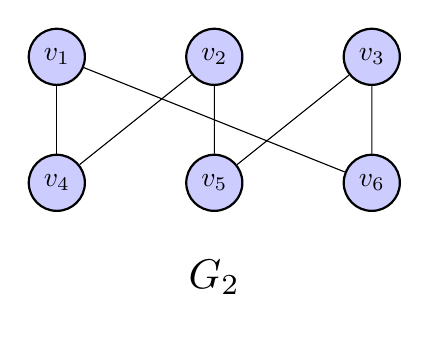
\begin{tikzpicture}
  [scale=.8,auto=left,every node/.style={circle,fill=blue!20,draw=black,thick}]
  
  % Fila superior (equivalente a la columna izquierda original)
  \node (n1) at (0,2) {$v_1$};
  \node (n2) at (2.5,2) {$v_2$};
  \node (n3) at (5,2) {$v_3$};

  % Fila inferior (equivalente a la columna derecha original)
  \node (n4) at (0,0) {$v_4$};
  \node (n5) at (2.5,0) {$v_5$};
  \node (n6) at (5,0) {$v_6$};

  % Aristas correspondientes a la imagen original
  \foreach \from/\to in {n1/n4, n1/n6, n2/n4, n2/n5, n3/n5, n3/n6}
    \draw (\from) -- (\to);

  % Etiqueta G_2 debajo del grafo
  \node[draw=none, fill=none, scale=1.5] at (2.5,-1.5) {$G_2$};

\end{tikzpicture}
}}%
 \hspace{2cm}%
 \makebox[0.3\textwidth]{\resizebox{0.25\textwidth}{!}{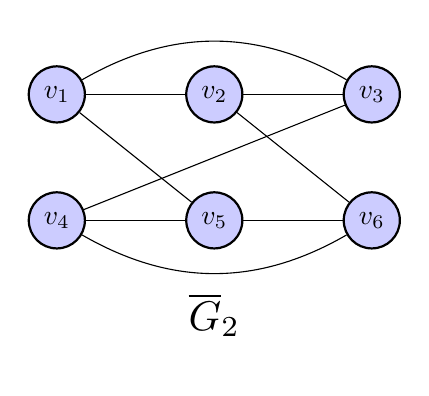
\begin{tikzpicture}
  [scale=.8,auto=left,every node/.style={circle,fill=blue!20,draw=black,thick}]
  
  % Fila superior
  \node (n1) at (0,2) {$v_1$};
  \node (n2) at (2.5,2) {$v_2$};
  \node (n3) at (5,2) {$v_3$};

  % Fila inferior
  \node (n4) at (0,0) {$v_4$};
  \node (n5) at (2.5,0) {$v_5$};
  \node (n6) at (5,0) {$v_6$};

  % Aristas del complemento \overline{G}_2
  % Conexiones dentro de la misma fila
  \draw (n1) to[bend left=30] (n3);
  \draw (n1) -- (n2);
  \draw (n2) -- (n3);
  
  \draw (n4) to[bend right=30] (n6);
  \draw (n4) -- (n5);
  \draw (n5) -- (n6);

  % Conexiones entre filas que faltaban en G_2
  \draw (n1) -- (n5);
  \draw (n2) -- (n6);
  \draw (n3) -- (n4);

  % Etiqueta \overline{G}_2 debajo del grafo
  \node[draw=none, fill=none, scale=1.5] at (2.5,-1.5) {$\overline{G}_2$};

\end{tikzpicture}
}}\par
 \captionof{figure}{Grafos y sus complementos}
\par}
\vspace{1em}

\end{Ejm}
Ahora procedemos a enunciar algunas clases especiales de grafos.
\begin{Def}
   Sea $G$ un grafo. Decimos que $G$ es \textbf{completo} si $V(G)$ es un clique. Un grafo completo con $n$ vértices se denota como $\bm{K^n}$.
\end{Def}
Por tanto, un grafo es completo si todos sus vértices son adyacentes dos a dos.
\begin{Ejm}
   El grafo vacío y el grafo con un solo vértice son grafos completos, que se denotan por $K^0$ y $K^1$, respectivamente. A continuación se muestran grafos completos con $3$, $5$ y $7$ vértices.
   \begin{figure}[H]
  \renewcommand{\diagscale}{0.2\textwidth}%
   \centering
   \resizebox{\diagscale}{!}{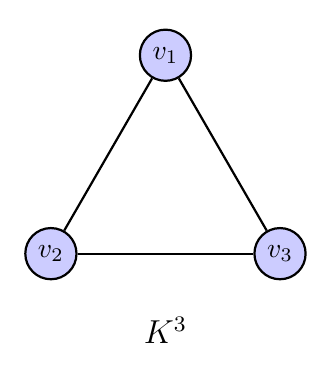
\begin{tikzpicture}[
  baseline=0pt,
  scale=0.7,
  vnode/.style={circle, draw=black, fill=blue!20, thick, inner sep=0pt, minimum size=6.5mm},
  edge/.style={thick, draw=black}
]
  \useasboundingbox (-2.5,-3.4) rectangle (2.5,2.3);

  % v1 en y=1.8, vértices inferiores en y=-1.8
  \node[vnode] (v1) at ([yshift=-0.6cm]90:2.4) {$v_1$};
  \node[vnode] (v2) at ([yshift=-0.6cm]210:2.4) {$v_2$};
  \node[vnode] (v3) at ([yshift=-0.6cm]330:2.4) {$v_3$};

  % Aristas
  \draw[edge] (v1) -- (v2);
  \draw[edge] (v2) -- (v3);
  \draw[edge] (v3) -- (v1);

  % Etiqueta
  \node[font=\large] at (0,-3.2) {$K^3$};
\end{tikzpicture}
}\hspace{4em}
   \resizebox{\diagscale}{!}{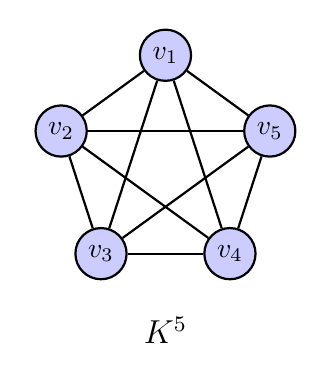
\begin{tikzpicture}[
  baseline=0pt,
  scale=0.7,
  vnode/.style={circle, draw=black, fill=blue!20, thick, inner sep=0pt, minimum size=6.5mm},
  edge/.style={thick, draw=black}
]
  \useasboundingbox (-2.5,-3.4) rectangle (2.5,2.3);

  % v1 en y=1.8, vértices inferiores en y=-1.8
  \node[vnode] (v1) at ([yshift=-0.19cm]90:1.99) {$v_1$};
  \node[vnode] (v2) at ([yshift=-0.19cm]162:1.99) {$v_2$};
  \node[vnode] (v3) at ([yshift=-0.19cm]234:1.99) {$v_3$};
  \node[vnode] (v4) at ([yshift=-0.19cm]306:1.99) {$v_4$};
  \node[vnode] (v5) at ([yshift=-0.19cm]18:1.99) {$v_5$};

  % Aristas
  \draw[edge] (v1) -- (v2); \draw[edge] (v1) -- (v3); \draw[edge] (v1) -- (v4); \draw[edge] (v1) -- (v5);
  \draw[edge] (v2) -- (v3); \draw[edge] (v2) -- (v4); \draw[edge] (v2) -- (v5);
  \draw[edge] (v3) -- (v4); \draw[edge] (v3) -- (v5);
  \draw[edge] (v4) -- (v5);

  % Etiqueta
  \node[font=\large] at (0,-3.2) {$K^5$};
\end{tikzpicture}
}\hspace{4em}
   \resizebox{\diagscale}{!}{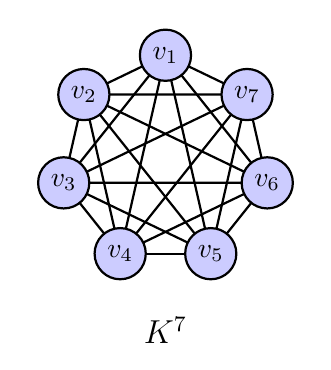
\begin{tikzpicture}[
  baseline=0pt,
  scale=0.7,
  vnode/.style={circle, draw=black, fill=blue!20, thick, inner sep=0pt, minimum size=6.5mm},
  edge/.style={thick, draw=black}
]
  \useasboundingbox (-2.5,-3.4) rectangle (2.5,2.3);

  \begin{scope}[yshift=-0.094cm]
    % Coordenadas con ángulos exactos
    \foreach \i in {1,...,7} {
      \pgfmathsetmacro{\ang}{90 + (\i-1)*360/7}
      \coordinate (v\i) at (\ang:1.894);
    }

    % Aristas
    \foreach \i in {1,...,6} {
      \pgfmathtruncatemacro{\start}{\i+1}
      \foreach \j in {\start,...,7} {
        \draw[edge] (v\i) -- (v\j);
      }
    }

    % Vértices
    \foreach \i in {1,...,7} {
      \node[vnode] at (v\i) {$v_\i$};
    }
  \end{scope}

  % Etiqueta
  \node[font=\large] at (0,-3.2) {$K^7$};
\end{tikzpicture}
}\vspace{0.5em}
 \caption{Ejemplos de grafos completos}
\end{figure}

\end{Ejm}
Para introducir los grafos conocidos como \textit{ciclos}, primero damos la siguiente definición.
\begin{Def}
   Sean $G$ un grafo y $F\subseteq [V(G)]^2$. Definimos el nuevo grafo $\bm{G+F}:=(V,E\cup F)$.
\end{Def}
De esta manera, lo que hacemos es adicionar a $G$, como nuevas aristas, las parejas de vértices que contenga $F$.
\begin{Ejm}
   \phantom{0}
   \begin{itemize}
      \item Si $F=\left\lbrace \left\lbrace v_2,v_6\right\rbrace, \left\lbrace v_2,v_5\right\rbrace, \left\lbrace v_3,v_6\right\rbrace, \left\lbrace v_3,v_5\right\rbrace\right\rbrace$ entonces:  
         \begin{figure}[H]
  \centering
  \resizebox{0.2\textwidth}{!}{\begin{tikzpicture}
  [scale=.6, auto=left, 
   vertex/.style={circle, fill=blue!20, draw=black, thick, inner sep=2pt, minimum size=18pt},
   edge/.style={thick, draw=black}]

  % Vértices
  \node[vertex] (n1) at (2,4) {$\scriptstyle v_1$};
  \node[vertex] (n2) at (4,3) {$\scriptstyle v_2$};
  \node[vertex] (n3) at (4,1) {$\scriptstyle v_3$};
  \node[vertex] (n4) at (2,0) {$\scriptstyle v_4$};
  \node[vertex] (n5) at (0,1) {$\scriptstyle v_5$};
  \node[vertex] (n6) at (0,3) {$\scriptstyle v_6$};

  % Aristas del grafo base G_2
  \foreach \from/\to in {n1/n2, n2/n3, n1/n3, n1/n4, n2/n4, n3/n4, n5/n6}
    \draw[edge] (\from) -- (\to);

  % Etiqueta inferior
    \node at (2,-1.5) {\large{$G_2$}};
\end{tikzpicture}
} \hspace{2cm}
  \resizebox{0.2\textwidth}{!}{\begin{tikzpicture}
  [scale=.6, auto=left, 
   vertex/.style={circle, fill=blue!20, draw=black, thick, inner sep=2pt, minimum size=18pt},
   edge/.style={thick, draw=black},
   bold_edge/.style={line width=2.5pt, draw=black}]

  % Vértices
  \node[vertex] (n1) at (2,4) {$\scriptstyle v_1$};
  \node[vertex] (n2) at (4,3) {$\scriptstyle v_2$};
  \node[vertex] (n3) at (4,1) {$\scriptstyle v_3$};
  \node[vertex] (n4) at (2,0) {$\scriptstyle v_4$};
  \node[vertex] (n5) at (0,1) {$\scriptstyle v_5$};
  \node[vertex] (n6) at (0,3) {$\scriptstyle v_6$};

  % Aristas normales de G_2
  \foreach \from/\to in {n1/n2, n2/n3, n1/n3, n1/n4, n2/n4, n3/n4, n5/n6}
    \draw[edge] (\from) -- (\to);

  % Aristas reteñidas de F: {v3,v6}, {v3,v5}, {v2,v6}, {v2,v5}
  \foreach \from/\to in {n3/n6, n3/n5, n2/n6, n2/n5}
    \draw[edge] (\from) -- (\to);

  % Etiqueta inferior
    \node at (2,-1.5) {\large{$G_2 + F$}};
\end{tikzpicture}
} 
    \caption{$G_2$ y $G_2+F$}
\end{figure}
  
      \item Si $F'=\left\lbrace \left\lbrace v_2,v_3\right\rbrace, \left\lbrace v_3,v_4\right\rbrace, \left\lbrace v_4,v_5\right\rbrace, \left\lbrace v_5,v_6 \right\rbrace\right\rbrace$ entonces:
         \vspace{1em}
         \begin{figure}[H]
  \centering
  \resizebox{0.2\textwidth}{!}{\begin{tikzpicture}
  [scale=.6, auto=left, 
   vertex/.style={circle, fill=blue!20, draw=black, thick, inner sep=2pt, minimum size=18pt},
   edge/.style={thick, draw=black}]

  % Vértices
  \node[vertex] (n1) at (2,4) {$\scriptstyle v_1$};
  \node[vertex] (n2) at (4,3) {$\scriptstyle v_2$};
  \node[vertex] (n3) at (4,1) {$\scriptstyle v_3$};
  \node[vertex] (n4) at (2,0) {$\scriptstyle v_4$};
  \node[vertex] (n5) at (0,1) {$\scriptstyle v_5$};
  \node[vertex] (n6) at (0,3) {$\scriptstyle v_6$};

  % Aristas del grafo G_3
  \foreach \from/\to in {n1/n2, n1/n3, n1/n4, n1/n5, n1/n6}
    \draw[edge] (\from) -- (\to);

  % Etiqueta inferior
    \node at (2,-1.5) {\large{$G_3$}};
\end{tikzpicture}
} \hspace{2cm}
  \resizebox{0.2\textwidth}{!}{\begin{tikzpicture}
  [scale=.6, auto=left, 
   vertex/.style={circle, fill=blue!20, draw=black, thick, inner sep=2pt, minimum size=18pt},
   edge/.style={thick, draw=black}]

  % Vértices
  \node[vertex] (n1) at (2,4) {$\scriptstyle v_1$};
  \node[vertex] (n2) at (4,3) {$\scriptstyle v_2$};
  \node[vertex] (n3) at (4,1) {$\scriptstyle v_3$};
  \node[vertex] (n4) at (2,0) {$\scriptstyle v_4$};
  \node[vertex] (n5) at (0,1) {$\scriptstyle v_5$};
  \node[vertex] (n6) at (0,3) {$\scriptstyle v_6$};

  % Aristas originales de G_3
  \foreach \from/\to in {n1/n2, n1/n3, n1/n4, n1/n5, n1/n6}
    \draw[edge] (\from) -- (\to);

  % Aristas añadidas: {v2,v3}, {v3,v4}, {v4,v5}, {v5,v6}
  \foreach \from/\to in {n2/n3, n3/n4, n4/n5, n5/n6}
    \draw[edge] (\from) -- (\to);

  % Etiqueta inferior
    \node at (2,-1.5) {\large{$G_3+F'$}};
\end{tikzpicture}
} 
    \caption{$G_3$ y $G_3+F'$}
\end{figure}
  
   \end{itemize}
\end{Ejm}
\begin{Def}
   Sea $P=x_0\dots x_{k-1}$ un camino, con $k\geq 3$. Decimos que el grafo $C:=P+\left\lbrace \left\lbrace x_{k-1}, x_0\right\rbrace\right\rbrace$ es llamado un \textbf{ciclo}. En este caso denotamos a $C$ mediante $x_0x_1\dots x_{k-1}x_0$. La \textbf{longitud} de un ciclo es su número de aristas (que es igual a su número de vértices). Un ciclo de longitud $k$ es llamado un $\bm{k-ciclo}$ y es denotado por $\bm{C^k}$. 
\end{Def}
\begin{Ejm}
   Se tiene que $C^3=K^3$; éste es el ciclo de menor longitud posible. A continuación mostramos los ciclos de longitud $4$, $6$ y $8$.
   \begin{figure}[H]
  \renewcommand{\diagscale}{0.2\textwidth}%
   \centering
   \resizebox{\diagscale}{!}{\begin{tikzpicture}[
  baseline=0pt,
  scale=0.7,
  vnode/.style={circle, draw=black, fill=blue!20, thick, inner sep=0pt, minimum size=6.5mm},
  edge/.style={thick, draw=black}
]
  \useasboundingbox (-2.3,-3.1) rectangle (2.3,2.4);

  % Vértices en radio 2.0 cm (v1 a 90°, v3 a 270°)
  \node[vnode] (v1) at (90:2.0) {$v_1$};
  \node[vnode] (v2) at (180:2.0) {$v_4$};
  \node[vnode] (v3) at (270:2.0) {$v_3$};
  \node[vnode] (v4) at (0:2.0) {$v_2$};

  % Aristas del ciclo C^4
  \draw[edge] (v1) -- (v2) -- (v3) -- (v4) -- (v1);

  % Etiqueta inferior en tamaño normal
  \node at (0,-3.4) {\large{$C^4$}};
\end{tikzpicture}
}\hspace{4em}
   \resizebox{\diagscale}{!}{\begin{tikzpicture}[
  baseline=0pt,
  scale=0.7,
  vnode/.style={circle, draw=black, fill=blue!20, thick, inner sep=0pt, minimum size=6.5mm},
  edge/.style={thick, draw=black}
]
  \useasboundingbox (-2.3,-3.7) rectangle (2.3,2.4);

  % Vértices en radio 2.0 cm (v1 a 90°, aumentando en sentido horario)
  \foreach \i in {1,...,6} {
    \pgfmathsetmacro{\ang}{90 - (\i-1)*360/6}
    \node[vnode] (v\i) at (\ang:2.0) {$v_\i$};
  }

  % Aristas del ciclo C^6
  \draw[edge] (v1) -- (v2) -- (v3) -- (v4) -- (v5) -- (v6) -- (v1);

  % Etiqueta inferior en tamaño normal
  \node at (0,-3.4) {\large{$C^6$}};
\end{tikzpicture}
}\hspace{4em}
   \resizebox{\diagscale}{!}{\begin{tikzpicture}[
  baseline=0pt,
  scale=0.7,
  vnode/.style={circle, draw=black, fill=blue!20, thick, inner sep=0pt, minimum size=6.5mm},
  edge/.style={thick, draw=black}
]
  \useasboundingbox (-2.3,-3.7) rectangle (2.3,2.4);

  % Vértices en radio 2.0 cm (v1 a 90°, aumentando en sentido horario)
  \foreach \i in {1,...,8} {
    \pgfmathsetmacro{\ang}{90 - (\i-1)*360/8}
    \node[vnode] (v\i) at (\ang:2.0) {$v_\i$};
  }

  % Aristas del ciclo C^8
  \draw[edge] (v1) -- (v2) -- (v3) -- (v4) -- (v5) -- (v6) -- (v7) -- (v8) -- (v1);

  % Etiqueta inferior en tamaño normal
  \node at (0,-3.4) {\large{$C^8$}};
\end{tikzpicture}
}\vspace{1.3em}
 \caption{Ejemplos de ciclos}
\end{figure}

\end{Ejm}
Los ciclos nos permiten definir fácilmente lo que es un \textit{árbol}.
\begin{Def}
   Un grafo conexo que no contiene ningún ciclo es llamado un \textbf{árbol}. 
\end{Def}
\begin{Ejm}
   Todos los caminos son ejemplos de árboles. Los únicos grafos completos que son árboles son $K^1$ y $K^2$; el grafo $K^0=\emptyset$ no es un árbol porque no es conexo, y cualquier grafo completo con $3$ o más vértices contiene a $C^3$. En la \Cref{fig:arboles_ejemplos} los grafos $T_1$, $T_2$ y $T_3$ son ejemplos de árboles.
   \begin{figure}[H]
  \centering
  \begin{tikzpicture}[
  baseline=0pt,
  scale=1,
  vnode/.style={circle, draw=black, fill=blue!20, thick, inner sep=0pt, minimum size=4.5mm},
  edge/.style={thick, draw=black}
]
  \useasboundingbox (-2.3,-3.1) rectangle (2.3,2.4);

  % 4 vértices (Estrella / Tridente)
  \node[vnode] (v1) at (0, 1.8) {};     % Vértice superior
  \node[vnode] (v2) at (0, 0.0) {};     % Vértice central
  \node[vnode] (v3) at (-1.4, -1.8) {}; % Vértice inferior izq
  \node[vnode] (v4) at (1.4, -1.8) {};  % Vértice inferior der

  % Aristas
  \draw[edge] (v2) -- (v1);
  \draw[edge] (v2) -- (v3);
  \draw[edge] (v2) -- (v4);

  % Etiqueta
  \node[font=\large] at (0,-2.7) {$T_1$};
\end{tikzpicture}
\hfill
  \begin{tikzpicture}[
  baseline=0pt,
  scale=1,
  vnode/.style={circle, draw=black, fill=blue!20, thick, inner sep=0pt, minimum size=4.5mm},
  edge/.style={thick, draw=black}
]
  \useasboundingbox (-2.3,-3.1) rectangle (2.3,2.4);

  % Reflejos verticales manteniendo los límites y=-1.8 y y=1.8
  \begin{scope}[yscale=-1]
    \node[vnode] (v1) at (0.5, 1.8) {};
    \node[vnode] (v2) at (0.0, 1.2) {};
    \node[vnode] (v3) at (1.1, 1.4) {};
    \node[vnode] (v4) at (1.8, 1.7) {};
    \node[vnode] (v5) at (1.6, 0.9) {};
    \node[vnode] (v6) at (-0.7, 0.9) {};
    \node[vnode] (v7) at (0.2, 0.4) {};
    \node[vnode] (v8) at (-1.5, 1.3) {};
    \node[vnode] (v9) at (-1.6, 0.5) {};
    \node[vnode] (v10) at (-0.9, -0.1) {};
    \node[vnode] (v11) at (0.8, -0.2) {};
    \node[vnode] (v12) at (-0.1, -0.4) {};
    \node[vnode] (v13) at (1.5, -0.6) {};
    \node[vnode] (v14) at (0.9, -1.1) {};
    \node[vnode] (v15) at (-0.8, -1.0) {};
    \node[vnode] (v16) at (-0.1, -1.2) {};
    \node[vnode] (v17) at (-1.6, -1.5) {};
    \node[vnode] (v18) at (-0.8, -1.8) {};
    \node[vnode] (v19) at (0.0, -1.8) {};
    \node[vnode] (v20) at (0.8, -1.7) {};

    % Aristas
    \draw[edge] (v1) -- (v2); \draw[edge] (v1) -- (v3);
    \draw[edge] (v3) -- (v4); \draw[edge] (v3) -- (v5);
    \draw[edge] (v2) -- (v6); \draw[edge] (v2) -- (v7);
    \draw[edge] (v6) -- (v8); \draw[edge] (v6) -- (v9); \draw[edge] (v6) -- (v10);
    \draw[edge] (v7) -- (v11); \draw[edge] (v7) -- (v12);
    \draw[edge] (v11) -- (v13); \draw[edge] (v11) -- (v14);
    \draw[edge] (v12) -- (v15); \draw[edge] (v12) -- (v16);
    \draw[edge] (v15) -- (v17); \draw[edge] (v15) -- (v18);
    \draw[edge] (v16) -- (v19); \draw[edge] (v16) -- (v20);
  \end{scope}

  % Etiqueta
  \node[font=\large] at (0,-2.7) {$T_2$};
\end{tikzpicture}
\hfill
  \begin{tikzpicture}[
  baseline=0pt,
  scale=1,
  vnode/.style={circle, draw=black, fill=blue!20, thick, inner sep=0pt, minimum size=4.5mm},
  edge/.style={thick, draw=black}
]
  \useasboundingbox (-2.3,-3.1) rectangle (2.3,2.4);

  % Posicionamiento de los 13 vértices
  \node[vnode] (u1) at (-0.5, 1.8) {};   % Vértice superior
  \node[vnode] (u2) at (0.0, 1.2) {};
  \node[vnode] (u3) at (0.8, 1.6) {};
  \node[vnode] (u4) at (-0.8, 0.6) {};
  \node[vnode] (u5) at (-1.6, 0.9) {};
  \node[vnode] (u6) at (-0.2, 0.0) {};
  \node[vnode] (u7) at (0.6, -0.4) {};
  \node[vnode] (u8) at (1.4, -0.2) {};
  \node[vnode] (u9) at (1.2, -1.0) {};
  \node[vnode] (u10) at (-0.6, -0.7) {};
  \node[vnode] (u11) at (-1.4, -1.2) {};
  \node[vnode] (u12) at (-0.5, -1.8) {}; % Vértice inferior 1
  \node[vnode] (u13) at (0.5, -1.8) {};  % Vértice inferior 2

  % Aristas (12 conexiones)
  \draw[edge] (u2) -- (u1);
  \draw[edge] (u2) -- (u3);
  \draw[edge] (u2) -- (u4); \draw[edge] (u4) -- (u5);
  \draw[edge] (u2) -- (u6);
  \draw[edge] (u6) -- (u7); \draw[edge] (u7) -- (u8); \draw[edge] (u7) -- (u9);
  \draw[edge] (u6) -- (u10); \draw[edge] (u10) -- (u11); \draw[edge] (u10) -- (u12);
  \draw[edge] (u6) -- (u13);

  % Etiqueta
  \node[font=\large] at (0,-2.7) {$T_3$};
\end{tikzpicture}

  \caption{Ejemplos de árboles}
  \label{fig:arboles_ejemplos}
\end{figure}

   En la \Cref{fig:no_arboles}, el grafo $S_1$ no es un árbol porque no es conexo; el grafo $S_2$ no es un árbol porque contiene el ciclo $C^5$.
   \begin{figure}[H]
  \centering
  \begin{tikzpicture}[
  baseline=0pt,
  scale=1,
  vnode/.style={circle, draw=black, fill=blue!20, thick, inner sep=0pt, minimum size=4.5mm},
  edge/.style={thick, draw=black}
]
  \useasboundingbox (-2.3,-3.1) rectangle (2.3,2.4);

  % --- ÁRBOL 1 (10 vértices, trazado orgánico) ---
  \node[vnode] (t1_1) at (-1.2, 1.8) {};   % Vértice superior
  \node[vnode] (t1_2) at (-1.7, 1.1) {};
  \node[vnode] (t1_3) at (-0.7, 1.2) {};
  \node[vnode] (t1_4) at (-2.0, 0.3) {};
  \node[vnode] (t1_5) at (-1.3, 0.4) {};
  \node[vnode] (t1_6) at (-0.4, 0.5) {};
  \node[vnode] (t1_7) at (-1.6, -0.4) {};
  \node[vnode] (t1_8) at (-0.9, -0.3) {};
  \node[vnode] (t1_9) at (-1.8, -1.8) {};  % Vértice inferior
  \node[vnode] (t1_10) at (-1.0, -1.2) {};

  \draw[edge] (t1_1) -- (t1_2); \draw[edge] (t1_1) -- (t1_3);
  \draw[edge] (t1_2) -- (t1_4); \draw[edge] (t1_2) -- (t1_5);
  \draw[edge] (t1_3) -- (t1_6);
  \draw[edge] (t1_5) -- (t1_7); \draw[edge] (t1_5) -- (t1_8);
  \draw[edge] (t1_7) -- (t1_9); \draw[edge] (t1_8) -- (t1_10);

  % --- ÁRBOL 2 (5 vértices, trazado orgánico) ---
  \node[vnode] (t2_1) at (1.2, 1.1) {};
  \node[vnode] (t2_2) at (0.7, 0.2) {};
  \node[vnode] (t2_3) at (1.7, 0.3) {};
  \node[vnode] (t2_4) at (1.0, -0.7) {};
  \node[vnode] (t2_5) at (1.5, -1.8) {};   % Vértice inferior

  \draw[edge] (t2_2) -- (t2_1);
  \draw[edge] (t2_2) -- (t2_3);
  \draw[edge] (t2_2) -- (t2_4);
  \draw[edge] (t2_4) -- (t2_5);

  % Etiqueta
  \node[font=\large] at (0,-2.7) {$S_1$};
\end{tikzpicture}
\hspace{6em}
  \begin{tikzpicture}[
  baseline=0pt,
  scale=1,
  vnode/.style={circle, draw=black, fill=blue!20, thick, inner sep=0pt, minimum size=4.5mm},
  edge/.style={thick, draw=black},
  bold_edge/.style={line width=2.5pt, draw=black}
]
  \useasboundingbox (-2.3,-3.1) rectangle (2.3,2.4);

  % --- CICLO C^5 (Ubicado en la esquina inferior derecha) ---
  % c3 y c4 son los ÚNICOS dos vértices sin ramas adicionales (grado 2)
  \node[vnode] (c1) at (0.4, -0.5) {};   % Conecta con Rama 1 (Arriba-Izquierda)
  \node[vnode] (c2) at (1.2, -0.5) {};   % Conecta con Rama 2 (Arriba-Derecha)
  \node[vnode] (c3) at (1.7, -1.1) {};   % Vértice limpio (grado 2)
  \node[vnode] (c4) at (1.1, -1.8) {};   % Vértice limpio (grado 2, límite inferior)
  \node[vnode] (c5) at (0.3, -1.2) {};   % Conecta con Rama 3 (Abajo-Izquierda)

  % Aristas del C^5 (reteñidas)
  \draw[bold_edge] (c1) -- (c2) -- (c3) -- (c4) -- (c5) -- (c1);

  % --- RAMA 1: Sale de c5 (3 vértices hacia abajo/izquierda) ---
  \node[vnode] (v6) at (-0.4, -1.2) {};
  \node[vnode] (v7) at (-1.1, -1.8) {};  % Límite inferior
  \node[vnode] (v8) at (-0.3, -1.8) {};  % Límite inferior

  \draw[edge] (c5) -- (v6);
  \draw[edge] (v6) -- (v7);
  \draw[edge] (v6) -- (v8);

  % --- RAMA 2: Sale de c2 (3 vértices hacia la derecha/arriba) ---
  \node[vnode] (v9)  at (1.8, -0.1) {};
  \node[vnode] (v10) at (1.9, 0.6) {};
  \node[vnode] (v11) at (1.4, 1.2) {};

  \draw[edge] (c2) -- (v9);
  \draw[edge] (v9) -- (v10);
  \draw[edge] (v10) -- (v11);

  % --- RAMA 3: Sale de c1 (9 vértices hacia arriba e izquierda) ---
  \node[vnode] (v12) at (-0.3, 0.0) {};
  \node[vnode] (v13) at (-1.1, 0.2) {};
  \node[vnode] (v14) at (-1.7, 0.7) {};
  \node[vnode] (v15) at (-1.0, 0.8) {};
  \node[vnode] (v16) at (0.3, 0.6) {};
  \node[vnode] (v17) at (-0.3, 1.2) {};
  \node[vnode] (v18) at (-1.1, 1.6) {};
  \node[vnode] (v19) at (-0.4, 1.8) {};  % Límite superior
  \node[vnode] (v20) at (0.5, 1.8) {};   % Límite superior

  \draw[edge] (c1) -- (v12);
  \draw[edge] (v12) -- (v13);
  \draw[edge] (v13) -- (v14);
  \draw[edge] (v13) -- (v15);
  \draw[edge] (v12) -- (v16);
  \draw[edge] (v16) -- (v17);
  \draw[edge] (v17) -- (v18);
  \draw[edge] (v17) -- (v19);
  \draw[edge] (v16) -- (v20);

  % Etiqueta
  \node[font=\large] at (0,-2.7) {$S_2$};
\end{tikzpicture}

  \caption{Ejemplos de grafos que no son árboles}
  \label{fig:no_arboles}
\end{figure}

\end{Ejm}
\begin{Def}
   Sea $G$ un grafo de orden mayor o igual que $2$. Decimos que $G$ es \textbf{bipartito} si $V(G)$ admite una partición en dos clases $V_1$ y $V_2$ tales que $V_1$ y $V_2$ son conjuntos independientes. Si además cualesquiera dos vértices de distintas clases de la partición son adyacentes, decimos que $G$ es \textbf{bipartito completo}, y denotamos a $G$ por $K_{n_1,n_2}$, donde $n_1=|V_1|$ y $n_2=|V_2|$. Grafos de la forma $K_{1,n}$ con $n\in \mathbb{Z}^+$ son llamados \textbf{estrellas}.
\end{Def}
De esta forma, en un grafo bipartito con partición de vértices $\left\lbrace V_1,V_2\right\rbrace$, cada vértice de $V_1$ puede ser adyacente únicamente a vértices de $V_2$, y cada vértice de $V_2$ puede ser adyacente únicamente a vértices de $V_1$. Si el grafo es además bipartito completo, cada vértice de $V_1$ es adyacente a todos los vértices de $V_2$ (y por tanto cada vértice de $V_2$ es adyacente a todos los vértices de $V_1$).\\\\
Además, una estrella es un grafo con dos o más vértices en que un único vértice es adyacente a todos los demás, y las únicas aristas son las que permiten estas adyacencias.
\begin{Obs}
    Por convención, consideramos que el grafo vacío y el grafo $K^1$ son bipartitos. Esta precisión técnica es sumamente útil, pues evita tener que arrastrar condiciones de no trivialidad en los enunciados y demostraciones de teoremas en la teoría (por ejemplo, al caracterizar los grafos bipartitos como aquellos que no contienen ciclos de longitud impar, según la Proposición~1.6.1 de \cite{diestel2017}).
\end{Obs}
\begin{Ejm}
   La \Cref{fig:bipartitos_ejemplos} muestra el grafo bipartito $G_1$, que no es bipartito completo; el grafo bipartito completo $K_{3,5}$ y la estrella $K_{1,7}$. En cada grafo las respectivas particiones del conjunto de vértices son encerradas como en un diagrama de Venn.
   \begin{figure}[H]
  \centering
  \begin{tikzpicture}[
  baseline=0pt,
  scale=1,
  vnode/.style={circle, draw=black, fill=blue!20, thick, inner sep=0pt, minimum size=4.5mm},
  edge/.style={thick, draw=black}
]
  \useasboundingbox (-2.3,-3.1) rectangle (2.3,2.4);

  % Conjuntos de la partición (Venn)
  \draw[thick, draw=gray!70, fill=gray!10] (-1.2, 0) ellipse [x radius=0.65cm, y radius=2.15cm];
  \draw[thick, draw=gray!70, fill=gray!10] (1.2, 0) ellipse [x radius=0.65cm, y radius=2.15cm];

  % Vértices Partición Izquierda (3 vértices)
  \node[vnode] (a1) at (-1.2, 1.8) {};
  \node[vnode] (a2) at (-1.2, 0.0) {};
  \node[vnode] (a3) at (-1.2, -1.8) {}; % Tercer vértice (aislado)

  % Vértices Partición Derecha (4 vértices)
  \node[vnode] (b1) at (1.2, 1.8) {};
  \node[vnode] (b2) at (1.2, 0.6) {};
  \node[vnode] (b3) at (1.2, -0.6) {};
  \node[vnode] (b4) at (1.2, -1.8) {};

  % Aristas
  \draw[edge] (a1) -- (b1); 
  \draw[edge] (a1) -- (b2);
  \draw[edge] (a2) -- (b2); 
  \draw[edge] (a2) -- (b3); 
  \draw[edge] (a2) -- (b4); % Conexión añadida con el cuarto vértice de la derecha

  % Etiqueta inferior
  \node[font=\large] at (0,-2.7) {$G_1$};
\end{tikzpicture}
\hfill
  \begin{tikzpicture}[
  baseline=0pt,
  scale=1,
  vnode/.style={circle, draw=black, fill=blue!20, thick, inner sep=0pt, minimum size=4.5mm},
  edge/.style={thick, draw=black}
]
  \useasboundingbox (-2.3,-3.1) rectangle (2.3,2.4);

  % Conjuntos de la partición (Venn)
  \draw[thick, draw=gray!70, fill=gray!10] (-1.2, 0) ellipse [x radius=0.65cm, y radius=2.15cm];
  \draw[thick, draw=gray!70, fill=gray!10] (1.2, 0) ellipse [x radius=0.65cm, y radius=2.15cm];

  % Vértices Partición Izquierda (3 vértices)
  \node[vnode] (a1) at (-1.2, 1.8) {};
  \node[vnode] (a2) at (-1.2, 0.0) {};
  \node[vnode] (a3) at (-1.2, -1.8) {};

  % Vértices Partición Derecha (5 vértices)
  \node[vnode] (b1) at (1.2, 1.8) {};
  \node[vnode] (b2) at (1.2, 0.9) {};
  \node[vnode] (b3) at (1.2, 0.0) {};
  \node[vnode] (b4) at (1.2, -0.9) {};
  \node[vnode] (b5) at (1.2, -1.8) {};

  % Aristas (Todas las conexiones)
  \foreach \i in {1,2,3} {
    \foreach \j in {1,...,5} {
      \draw[edge] (a\i) -- (b\j);
    }
  }

  % Etiqueta inferior
  \node[font=\large] at (0,-2.7) {$K_{3,5}$};
\end{tikzpicture}
\hfill
  \begin{tikzpicture}[
  baseline=0pt,
  scale=1,
  vnode/.style={circle, draw=black, fill=blue!20, thick, inner sep=0pt, minimum size=4.5mm},
  edge/.style={thick, draw=black}
]
  \useasboundingbox (-2.3,-3.1) rectangle (2.3,2.4);

  % Partición 2 (Venn): Anillo exterior que encierra los 7 vértices
  \draw[thick, draw=gray!70, fill=gray!10, even odd rule] (0,0) circle (2.15cm) (0,0) circle (1.25cm);

  % Partición 1 (Venn): Círculo central que encierra el vértice central
  \draw[thick, draw=gray!70, fill=gray!10] (0,0) circle (0.65cm);

  % Vértice de la Partición 1 (Centro)
  \node[vnode] (a1) at (0, 0) {};

  % Vértices de la Partición 2 (7 vértices distribuidos uniformemente)
  \foreach \j in {1,...,7} {
    \pgfmathsetmacro{\ang}{90 + (\j-1)*360/7}
    \node[vnode] (b\j) at (\ang:1.8) {};
  }

  % Aristas desde el centro a cada vértice exterior
  \foreach \j in {1,...,7} {
    \draw[edge] (a1) -- (b\j);
  }

  % Etiqueta inferior
  \node[font=\large] at (0,-2.7) {$K_{1,7}$};
\end{tikzpicture}

  \caption{Ejemplos de grafos bipartitos}
  \label{fig:bipartitos_ejemplos}
\end{figure}

\end{Ejm}
La siguiente definición aborda el problema de la coloración de grafos.
\begin{Def}
   Sea $G$ un grafo. Una \textbf{coloración} de $G$ es una función $c: V(G) \to S$, donde $S$ es un conjunto cuyos elementos son llamados \textbf{colores}, tal que $c(u) \neq c(v)$ para cualesquiera dos vértices adyacentes $u, v \in V(G)$. Si el conjunto de colores $S$ tiene cardinalidad $k$, decimos que $c$ es una \textbf{$\bm{k}$-coloración}. Si $G$ tiene una \textbf{$\bm{k}$-coloración} decimos que $G$ es \textbf{$\bm{k}$-coloreable}. El menor cardinal $k$ para el cual existe una $k$-coloración de $G$ es el \textbf{número cromático} de $G$, el cual se denota por $\chi(G)$.
\end{Def}
Notemos que, para cualquier grafo $G$, la función identidad en $V(G)$ es una coloración de $G$; por tanto, todo grafo admite al menos una coloración y el número cromático $\chi(G)$ está bien definido. En particular, la función vacía de $\emptyset$ en $\emptyset$ es una coloración del grafo vacío, por lo que $\chi(\emptyset) = 0$. Para representar visualmente la coloración $c$ de un grafo, colocaremos la etiqueta correspondiente a $c(v)$ junto al círculo que representa al vértice $v$ (y no en su interior, para no confundirla con el vértice en sí). A continuación, mostramos algunos ejemplos de coloración de grafos.
\begin{Ejm}
   En la \Cref{tab:coloraciones_grafos}, para cada grafo $G_i$, con $i=1,2,3$, se tiene que $c_i$ es una coloración del grafo.
   \begin{longtable}{|S{c}|S{c}|S{c}|}
  % 1. DEFINIMOS EL PIE DE LA TABLA (AQUÍ VA EL CAPTION PARA QUE SALGA ABAJO)
  \hline
   \caption{Ejemplos de grafos con coloraciones}
  \addtocounter{table}{-1}\refstepcounter{table}% <-- Notifica a cleveref que es una tabla
  \label{tab:coloraciones_grafos} \\
  \endlastfoot
  
  % =========================================================
  % 2. A PARTIR DE AQUÍ VA EL CUERPO DE LA TABLA
  % =========================================================
  \hline
  % FILA 1: Nombres de los grafos
  \textbf{$G_1$} & \textbf{$G_2$} & \textbf{$G_3$} \\
  \hline
  
  % FILA 2: Grafos centrados en sus casillas
  \begin{tikzpicture}[
  baseline=0pt,
  scale=1,
  vnode/.style={circle, draw=black, fill=blue!20, thick, inner sep=0pt, minimum size=6.5mm},
  edge/.style={thick, draw=black},
  clabel/.style={font=\small, color=black}
]
  \useasboundingbox (-2.1,-2.3) rectangle (2.1,2.4);

  \begin{scope}[yshift=-0.2cm]
    % 7 Vértices
    \node[vnode, label={[clabel]above left:$1$}] (v1) at (0.0, 1.8) {$\scriptstyle v_1$};
    \node[vnode, label={[clabel]right:$2$}]        (v2) at (1.4, 0.9) {$\scriptstyle v_2$};
    \node[vnode, label={[clabel]right:$3$}]        (v3) at (1.4, -0.9) {$\scriptstyle v_3$};
    \node[vnode, label={[clabel]below:$4$}]        (v4) at (0.0, -1.8) {$\scriptstyle v_4$};
    \node[vnode, label={[clabel]left:$1$}]         (v5) at (-1.4, -0.9) {$\scriptstyle v_5$};
    \node[vnode, label={[clabel]left:$3$}]         (v6) at (-1.4, 0.9) {$\scriptstyle v_6$};
    \node[vnode, label={[clabel]above:$1$}]        (v7) at (0.0, 0.0) {$\scriptstyle v_7$};

    % Aristas
    \draw[edge] (v1) -- (v2) -- (v3) -- (v4) -- (v5) -- (v6) -- (v1);
    \draw[edge] (v7) -- (v2);
    \draw[edge] (v7) -- (v6);
    \draw[edge] (v7) -- (v4);
  \end{scope}
\end{tikzpicture}
 &
  \begin{tikzpicture}[
  baseline=0pt,
  scale=1,
  vnode/.style={circle, draw=black, fill=blue!20, thick, inner sep=0pt, minimum size=6.5mm},
  edge/.style={thick, draw=black},
  clabel/.style={font=\small, color=black}
]
  % Se amplía xmin a -2.55 para añadir el medio carácter de margen izquierdo
  \useasboundingbox (-2.55,-2.2) rectangle (2.25,2.3);

  \begin{scope}[yshift=-0.2cm]
    % --- COMPONENTE 1 ---
    \node[vnode, label={[clabel]above:$1$}] (v1) at (-1.2, 1.8) {$\scriptstyle v_1$};
    \node[vnode, label={[clabel]left:$2$}]  (v2) at (-1.8, 0.9) {$\scriptstyle v_2$};
    \node[vnode, label={[clabel]right:$3$}] (v3) at (-0.6, 0.9) {$\scriptstyle v_3$};
    \node[vnode, label={[clabel]left:$1$}]  (v4) at (-1.8, -0.4) {$\scriptstyle v_4$};
    \node[vnode, label={[clabel]right:$2$}] (v5) at (-0.6, -0.4) {$\scriptstyle v_5$};
    \node[vnode, label={[clabel]below:$3$}] (v6) at (-1.2, -1.8) {$\scriptstyle v_6$};

    \draw[edge] (v1) -- (v2) -- (v3) -- (v1);
    \draw[edge] (v2) -- (v4);
    \draw[edge] (v3) -- (v5);
    \draw[edge] (v4) -- (v5);
    \draw[edge] (v4) -- (v6);
    \draw[edge] (v5) -- (v6);

    % --- COMPONENTE 2 ---
    \node[vnode, label={[clabel]left:$1$}]  (v7)  at (1.2, 0.0) {$\scriptstyle v_7$};
    \node[vnode, label={[clabel]above:$2$}] (v8)  at (1.2, 1.8) {$\scriptstyle v_8$};
    \node[vnode, label={[clabel]below:$2$}] (v9)  at (0.5, -1.8) {$\scriptstyle v_9$};
    \node[vnode, label={[clabel]below:$2$}] (v10) at (1.9, -1.8) {$\scriptstyle v_{10}$};

    \draw[edge] (v7) -- (v8);
    \draw[edge] (v7) -- (v9);
    \draw[edge] (v7) -- (v10);
  \end{scope}
\end{tikzpicture}
 &
  \begin{tikzpicture}[
  baseline=0pt,
  scale=1,
  vnode/.style={circle, draw=black, fill=blue!20, thick, inner sep=0pt, minimum size=6.5mm},
  edge/.style={thick, draw=black},
  clabel/.style={font=\small, color=black}
]
  % Caja delimitadora simétrica (-1.8 a 1.8) para centrar el eje x = 0
  \useasboundingbox (-1.8,-2.8) rectangle (1.8,2.4);

  \begin{scope}[yshift=-0.2cm]
    % Primeros 5 vértices
    \node[vnode, label={[clabel]above:$1$}]        (v1) at (0.0, 1.8) {$\scriptstyle v_1$};
    \node[vnode, label={[clabel]left:$2$}]         (v2) at (-0.9, 0.9) {$\scriptstyle v_2$};
    \node[vnode, label={[clabel]right:$1$}]        (v3) at (0.9, 0.0) {$\scriptstyle v_3$};
    \node[vnode, label={[clabel]left:$2$}]         (v4) at (-0.9, -0.9) {$\scriptstyle v_4$};
    \node[vnode, label={[clabel]below left:$1$}] (v5) at (0.0, -1.8) {$\scriptstyle v_5$};

    % Aristas
    \draw[edge] (v1) -- (v2) -- (v3) -- (v4) -- (v5);
    \draw[edge] (v5) -- (1.2, -2.4);
    \node[font=\small] at (1.5, -2.4) {$\dots$};
  \end{scope}
\end{tikzpicture}
 \\
  \hline
  
  % FILA 3: Funciones alineadas
  $\begin{aligned}[t]
      c_1 \!:\phantom{o} V(G_1) &\to \{1, 2, 3, 4\} \\
     v_1 &\mapsto 1 \\
     v_2 &\mapsto 2 \\
     v_3 &\mapsto 3 \\
     v_4 &\mapsto 4 \\
     v_5 &\mapsto 1 \\
     v_6 &\mapsto 3 \\
     v_7 &\mapsto 1
  \end{aligned}$ 
  &
  $\begin{aligned}[t]
     c_2 \!:\phantom{o} V(G_2) &\to \{1, 2, 3\} \\
     v_1 &\mapsto 1 \\
     v_2 &\mapsto 2 \\
     v_3 &\mapsto 3 \\
     v_4 &\mapsto 1 \\
     v_5 &\mapsto 2 \\
     v_6 &\mapsto 3 \\
     v_7 &\mapsto 1 \\
     v_8 &\mapsto 2 \\
     v_9 &\mapsto 2 \\
     v_{10} &\mapsto 2
  \end{aligned}$ 
  &
  $\begin{aligned}[t]
     c_3 \!:\phantom{o} V(G_3) &\to \{1, 2\} \\
     v_i &\mapsto 
     \begin{cases} 
       1 & \begin{array}[t]{@{}l@{}} \text{si } i \text{ es} \\[-1ex] \text{impar} \end{array} \\[0.6ex]
       2 & \begin{array}[t]{@{}l@{}} \text{si } i \text{ es} \\[-1ex] \text{par} \end{array} 
     \end{cases}
  \end{aligned}$ \\
  \hline
\end{longtable}

\end{Ejm}

\subsection{Homomorfismos}
En lo que resta de esta sección nos ocuparemos de relacionar parejas de grafos mediante funciones.
\begin{Def}\label{Def:homomorfismo}
   Sean $G=(V,E)$ y $G'=(V',E')$ dos grafos. Decimos que $\varphi:V\to V'$ es un homomorfismo de $G$ en $G'$ si $\left\lbrace u,v\right\rbrace\in E$ implica $\left\lbrace \varphi(u),\varphi(v) \right\rbrace\in E'$ para cualesquiera vértices $u,v\in V$.
\end{Def}
El hecho de que $\left\lbrace u,v \right\rbrace\in E$ implique $\left\lbrace \varphi(u),\varphi(v)\right\rbrace\in E'$ lo resumimos diciendo que $\varphi$ preserva la adyacencia entre vértices, puesto que $\varphi$ envía vértices adyacentes de $G$ a vértices adyacentes de $G'$.
\begin{Ejm}\label{Ejm:homomorfismos}
   La función
   \begin{center}
   $\hfill
   \begin{array}{rcl}
      \varphi_1 \colon V(G) &\to& V(G') \\
      v_1 &\mapsto& w_1 \\
      v_2 &\mapsto& w_2 \\
      v_3 &\mapsto& w_3 \\
      v_4 &\mapsto& w_2 \\
      v_5 &\mapsto& w_1
   \end{array}
   \hfill$
   \end{center}
   es un homomorfismo de $G$ en $G'$, donde $G$ y $G'$ son los grafos que se muestran a continuación.
   \begin{figure}[H]
  \centering
  % Primer grafo (G_1)
  \begin{minipage}[t]{0.49\textwidth}
    \centering
    \scalebox{0.7}{% Ajusta este valor (ej. 0.6, 0.7, 0.8) para controlar el tamaño
      \begin{tikzpicture}[scale=.8,auto=left,every node/.style={circle,fill=blue!20,draw=black,thick}]
  % Vértices G1
  \node (n1) at (0, 4) {$v_1$};
  \node (n2) at (4, 4) {$v_2$};
  \node (n3) at (1.5, 2) {$v_3$};
  \node (n4) at (0, -1) {$v_4$};
  \node (n5) at (4, -1) {$v_5$};

  % Aristas G1 (Quitando n2/n4)
  \foreach \from/\to in {n1/n2, n1/n3, n1/n4, n2/n3, n2/n5, n3/n4}
    \draw (\from) -- (\to);

  % Título
  \node[draw=none, fill=none, scale=1.5] at (2, -2.5) {$G$};
\end{tikzpicture}

    }
  \end{minipage}%
  \hspace{-2em}%
  % Segundo grafo (G'_1)
  \begin{minipage}[t]{0.49\textwidth}
    \centering
    \scalebox{0.7}{% Usa el mismo factor de escala para que guarden proporción
      \begin{tikzpicture}[scale=.8,auto=left,every node/.style={circle,fill=blue!20,draw=black,thick}]
  % Vértices G'1
  \node (m1) at (0, 4) {$w_1$};
  \node (m2) at (0, -1) {$w_2$};
  \node (m3) at (2, 1.5) {$w_3$};
  \node (m4) at (5, 1.5) {$w_4$};

  % Aristas G'1
  \foreach \from/\to in {m1/m2, m1/m3, m1/m4, m2/m3, m2/m4, m3/m4}
    \draw (\from) -- (\to);

  % Título
  \node[draw=none, fill=none, scale=1.5] at (2.5, -2.5) {$G'$};
\end{tikzpicture}

    }
  \end{minipage}
  
  \caption{$\varphi$ es un homomorfismo de $G$ en $G'$}
  \label{fig:homomorfismo_grafos}
\end{figure}

   Para verificar que $\varphi_1$ es un homomorfismo notemos que $\varphi_1$ preserva la adyacencia entre vértices de $G$:
   \begin{center}
   $\hfill
   \begin{array}{rcl}
      \{v_1, v_2\} \in E(G) &\text{ y }& \{\varphi_1(v_1), \varphi_1(v_2)\} = \{w_1, w_2\} \in E(G'), \\
      \{v_1, v_3\} \in E(G) &\text{ y }& \{\varphi_1(v_1), \varphi_1(v_3)\} = \{w_1, w_3\} \in E(G'), \\
      \{v_1, v_4\} \in E(G) &\text{ y }& \{\varphi_1(v_1), \varphi_1(v_4)\} = \{w_1, w_2\} \in E(G'), \\
      \{v_2, v_3\} \in E(G) &\text{ y }& \{\varphi_1(v_2), \varphi_1(v_3)\} = \{w_2, w_3\} \in E(G'), \\
      \{v_2, v_5\} \in E(G) &\text{ y }& \{\varphi_1(v_2), \varphi_1(v_5)\} = \{w_2, w_1\} \in E(G'), \\
      \{v_3, v_4\} \in E(G) &\text{ y }& \{\varphi_1(v_3), \varphi_1(v_4)\} = \{w_3, w_2\} \in E(G').
   \end{array}
   \hfill$
   \end{center}
   En cambio la función
   \begin{center}
   $\hfill
   \begin{array}{rcl}
      \varphi_2 \colon V(G) &\to& V(G') \\
      v_1 &\mapsto& w_4 \\
      v_2 &\mapsto& w_2 \\
      v_3 &\mapsto& w_4 \\
      v_4 &\mapsto& w_1 \\
      v_5 &\mapsto& w_3
   \end{array}
   \hfill$
   \end{center}
   no es un homomorfismo de $G$ en $G'$, pues $\left\lbrace v_1,v_3\right\rbrace\in E(G)$ pero $\left\lbrace \varphi(v_1),\varphi(v_3)\right\rbrace=\left\lbrace w_4\right\rbrace\notin E(G')$.\\
   Podemos ver también que la función
   \begin{center}
   $\hfill
   \begin{array}{rcl}
      \psi \colon V(H) &\to& V(H') \\
      x_1 &\mapsto& y_1 \\
      x_2 &\mapsto& y_2 \\
      x_3 &\mapsto& y_3 \\
      x_4 &\mapsto& y_4 
   \end{array}
   \hfill$
   \end{center}
   es un homomorfismo entre los grafos $H$ y $H'$, que se presentan en la \Cref{fig:homomorfismo_grafos_2}
   \begin{figure}[H]
  \centering
  % Primer grafo (G_1)
  \begin{minipage}[t]{0.49\textwidth}
    \centering
    \scalebox{0.7}{% Ajusta este valor (ej. 0.6, 0.7, 0.8) para controlar el tamaño
      \begin{tikzpicture}[scale=.8,auto=left,every node/.style={circle,fill=blue!20,draw=black,thick}]
  % Vértices del cuadrado interior (C_4)
   \node (w1) at (-1, 1) {$x_1$};
  \node (w2) at (1, 1) {$x_2$};
  \node (w3) at (1, -1) {$x_3$};
  \node (w4) at (-1, -1) {$x_4$};

  % Vértices del cuadrado exterior (C_4 más grande)
  \node (w5) at (-2.5, 2.5) [opacity=0]{$w_5$};
  \node (w6) at (2.5, 2.5) [opacity=0]{$w_6$};
  \node (w7) at (2.5, -2.5) [opacity=0]{$w_7$};
  \node (w8) at (-2.5, -2.5) [opacity=0]{$w_8$};

  % Aristas del cuadrado interior
  \foreach \from/\to in {w1/w2, w2/w3, w3/w4, w4/w1}
    \draw (\from) -- (\to);

  % Título del grafo en la parte inferior
  \node[draw=none, fill=none, scale=1.5] at (0,-3.5) {$H$};
\end{tikzpicture}

    }
  \end{minipage}%
  \hspace{-3.5em}%
  % Segundo grafo (G'_1)
  \begin{minipage}[t]{0.49\textwidth}
    \centering
    \scalebox{0.7}{% Usa el mismo factor de escala para que guarden proporción
      \begin{tikzpicture}[scale=.8,auto=left,every node/.style={circle,fill=blue!20,draw=black,thick}]
  % Vértices del cuadrado interior (C_4)
  \node (w1) at (-1, 1) {$y_1$};
  \node (w2) at (1, 1) {$y_2$};
  \node (w3) at (1, -1) {$y_3$};
  \node (w4) at (-1, -1) {$y_4$};

  % Vértices del cuadrado exterior (C_4 más grande)
  \node (w5) at (-2.5, 2.5) {$y_5$};
  \node (w6) at (2.5, 2.5) {$y_6$};
  \node (w7) at (2.5, -2.5) {$y_7$};
  \node (w8) at (-2.5, -2.5) {$y_8$};

  % Aristas del cuadrado interior
  \foreach \from/\to in {w1/w2, w2/w3, w3/w4, w4/w1}
    \draw (\from) -- (\to);

  % Aristas del cuadrado exterior
  \foreach \from/\to in {w5/w6, w6/w7, w7/w8, w8/w5}
    \draw (\from) -- (\to);

  % Conexiones entre los vértices correspondientes de ambos cuadrados
  \foreach \from/\to in {w1/w5, w2/w6, w3/w7, w4/w8}
    \draw (\from) -- (\to);

  % Título del grafo en la parte inferior
  \node[draw=none, fill=none, scale=1.5] at (0,-3.5) {$H'$};
\end{tikzpicture}

    }
  \end{minipage}
  
  \caption{$H$ y $H'$}
  \label{fig:homomorfismo_grafos_2}
\end{figure}

   pues
   \begin{center}
   $\hfill
   \begin{array}{rcl}
      \{x_1, x_2\} \in E(H) &\text{ y }& \{\varphi_1(x_1), \varphi_1(x_2)\} = \{y_1, y_2\} \in E(H'), \\
      \{x_2, x_3\} \in E(H) &\text{ y }& \{\varphi_1(x_2), \varphi_1(x_3)\} = \{y_2, y_3\} \in E(H'), \\
      \{x_3, x_4\} \in E(H) &\text{ y }& \{\varphi_1(x_3), \varphi_1(x_4)\} = \{y_3, y_4\} \in E(H'), \\
      \{x_4, x_1\} \in E(H) &\text{ y }& \{\varphi_1(x_4), \varphi_1(x_1)\} = \{y_4, y_1\} \in E(H').
   \end{array}
   \hfill$
   \end{center}
\end{Ejm}
Estamos interesados en encontrar funciones entre vértices que permitan determinar si los grafos en cuestión son ``indistinguibles'' para la teoría construida. Un homomorfismo no es suficiente para esto: notemos que en la \Cref{Def:homomorfismo}, un homomorfismo puede enviar vértices no adyacentes en el grafo de partida a vértices adyacentes en el grafo de llegada. Como muestra de esto, en el \Cref{Ejm:homomorfismos}, se tiene que $\varphi_1$ es un homomorfismo de $G$ en $G'$, y a pesar de que $v_3$ y $v_5$ no son adyacentes en $G$, vemos que $\varphi_1(v_3)=w_3$ y $\varphi_1(v_5)=w_1$ sí son adyacentes en $G'$. Un primer paso sería exigir que la función, además de preservar la adyacencia de los vértices del grafo de partida, no envíe vértices no adyacentes en vértices adyacentes. Sin embargo, esta propiedad la cumple la función $\psi$ del \Cref{Ejm:homomorfismos}, conectando al grafo $H$ de $4$ vértices y $4$ aristas con el grafo $H'$ de $8$ vértices y $12$ aristas. Incluir la exigencia de que la función sea biyectiva solventa el problema y se obtiene la definición de \textit{isomorfismo} entre grafos.
\begin{Def}
   Sean $G=(V,E)$ y $G'=(V',E')$ dos grafos. Decimos que una función $\varphi:V\to V'$ es un \textbf{isomorfismo} de $G$ en $G'$ si $\varphi$ es biyectiva y $\left\lbrace u,v\right\rbrace\in E$, si y sólo si, $\left\lbrace \varphi(u), \varphi(v)\right\rbrace\in E'$, para cualesquiera vértices $u,v\in V$. Si existe un isomorfismo de $G$ en $G'$ decimos que $G$ y $G'$ son \textbf{isomorfos} y escribimos $G\simeq G'$. Un isomorfismo de $G$ en sí mismo es llamado un \textbf{automorfismo} de $G$.
\end{Def}
Usualmente no hacemos distinción alguna entre grafos isomorfos. Esto es lo que nos permite hablar de ``\textit{el} camino de $6$ vértices'', ``\textit{el} grafo completo de $4$ vértices'', etc.
\begin{Obs}
   En cualquier grafo $G$ la función identidad de $V(G)$ es un automorfismo de $G$.
\end{Obs}
\begin{Ejm}
   En la \Cref{fig:primer_isomorfismo} los grafos $G$ y $G'$ son isomorfos. 
   \begin{figure}[H]
  \centering
  % Primer grafo (G_1)
  \begin{minipage}[t]{0.49\textwidth}
    \centering
    \scalebox{0.7}{% Ajusta este valor (ej. 0.6, 0.7, 0.8) para controlar el tamaño
      \begin{tikzpicture}[auto=left,every node/.style={circle,fill=blue!20,draw=black,thick}]
  % Cuadrado exterior (v4 y v5 en la parte superior; v7 y v6 en la parte inferior)
  \node (v4) at (-3, 3.5) {$v_4$};
  \node (v5) at (3, 3.5) {$v_5$};
  \node (v6) at (3, -2.5) {$v_6$};
  \node (v7) at (-3, -2.5) {$v_7$};

  % Triángulo interior (v1, v2, v3)
  \node (v1) at (-1.5, 1.5) {$v_1$};
  \node (v2) at (1.5, 1.5) {$v_2$};
  \node (v3) at (0, -0.5) {$v_3$};

  % Aristas del cuadrado exterior
  \foreach \from/\to in {v4/v5, v5/v6, v6/v7, v7/v4}
    \draw (\from) -- (\to);

  % Aristas del triángulo interior
  \foreach \from/\to in {v1/v2, v2/v3, v3/v1}
    \draw (\from) -- (\to);

  % Conexiones del vértice inferior v3 a las esquinas inferiores
  \draw (v3) -- (v7);
  \draw (v3) -- (v6);

  % Título
  \node[draw=none, fill=none, scale=1.5] at (0,-3.8) {$G$};
\end{tikzpicture}

    }
  \end{minipage}%
  \hspace{-3em}%
  % Segundo grafo (G'_1)
  \begin{minipage}[t]{0.49\textwidth}
    \centering
    \scalebox{0.7}{% Usa el mismo factor de escala para que guarden proporción
      \begin{tikzpicture}[auto=left,every node/.style={circle,fill=blue!20,draw=black,thick}]
  % Vértice superior en la misma cota máxima (y=3.5)
  \node (w3) at (0, 3.5) {$w_3$};

  % "Casa" interior (w7, w6, w5, w4)
  \node (w7) at (-1.2, 1.5) {$w_7$};
  \node (w6) at (1.2, 1.5) {$w_6$};
  \node (w5) at (1.2, -0.5) {$w_5$};
  \node (w4) at (-1.2, -0.5) {$w_4$};

  % Vértices inferiores en la misma cota mínima (y=-2.5)
  \node (w1) at (-3, -2.5) {$w_1$};
  \node (w2) at (3, -2.5) {$w_2$};

  % Aristas de la estructura interior
  \foreach \from/\to in {w7/w6, w6/w5, w5/w4, w4/w7, w3/w7, w3/w6}
    \draw (\from) -- (\to);

  % Arista de la base exterior
  \draw (w1) -- (w2);

  % Arcos exteriores curvados
  \draw (w3) to[out=180, in=90] (w1);
  \draw (w3) to[out=0, in=90] (w2);

  % Título
  \node[draw=none, fill=none, scale=1.5] at (0,-3.8) {$G'$};
\end{tikzpicture}

    }
  \end{minipage}
  
  \caption{$G$ y $G'$ son isomorfos}
  \label{fig:primer_isomorfismo}
\end{figure}

   Consideremos la función $\varphi:V(G)\to V(G'):v_i\mapsto w_i$ para $i=1,2,\dots ,7$. Se tiene que $\varphi$ es biyectiva. Además
   \begin{center}
   $\hfill
   \begin{array}{rcl}
      \{v_1, v_2\} \in E(G) &\text{ y }& \{\varphi(v_1), \varphi(v_2)\} = \{w_1, w_2\} \in E(G'), \\
      \{v_1, v_3\} \in E(G) &\text{ y }& \{\varphi(v_1), \varphi(v_3)\} = \{w_1, w_3\} \in E(G'), \\
      \{v_2, v_3\} \in E(G) &\text{ y }& \{\varphi(v_2), \varphi(v_3)\} = \{w_2, w_3\} \in E(G'), \\
      \{v_3, v_7\} \in E(G) &\text{ y }& \{\varphi(v_3), \varphi(v_7)\} = \{w_3, w_7\} \in E(G'), \\
      \{v_3, v_6\} \in E(G) &\text{ y }& \{\varphi(v_3), \varphi(v_6)\} = \{w_3, w_6\} \in E(G'), \\
      \{v_6, v_7\} \in E(G) &\text{ y }& \{\varphi(v_6), \varphi(v_7)\} = \{w_6, w_7\} \in E(G'), \\
      \{v_4, v_7\} \in E(G) &\text{ y }& \{\varphi(v_4), \varphi(v_7)\} = \{w_4, w_7\} \in E(G'), \\
      \{v_4, v_5\} \in E(G) &\text{ y }& \{\varphi(v_4), \varphi(v_5)\} = \{w_4, w_5\} \in E(G'), \\
      \{v_5, v_6\} \in E(G) &\text{ y }& \{\varphi(v_5), \varphi(v_6)\} = \{w_5, w_6\} \in E(G').
   \end{array}
   \hfill$
   \end{center}
   Notemos que en la anterior lista se verifica tanto que $\left\lbrace u,v\right\rbrace\in E(G)$ implica $\left\lbrace \varphi(u), \varphi(v) \right\rbrace \allowbreak \in E(G')$, como que $\left\lbrace \varphi(u), \varphi(v)\right\rbrace\in E(G')$ implica $\left\lbrace u,v\right\rbrace\in E(G)$, para cualesquiera $u,v\in V(G)$. Por tanto $\varphi$ es un isomorfismo de $G$ en $G'$.
\end{Ejm}
El siguiente ejemplo muestra que no es suficiente que una función sea un homomorfismo biyectivo para que sea un isomorfismo.
\begin{Ejm}
   La función $\varphi:V(G)\to V(G'):v_i\mapsto w_i$ para $i=1,2$, es un homomorfismo biyectivo entre los grafos $G$ y $G'$ de la \Cref{fig:homomorfo_no_isomorfo}. Vacíamente se tiene que $\varphi$ preserva la adyacencia entre vértices.
   \begin{figure}[H]
\centering
  \resizebox{0.4\textwidth}{!}{\begin{tikzpicture}  
      [scale=.8,auto=left,every node/.style={circle,fill=blue!20,draw=black,thick}]
      \node (n1) at (0,0) {$v_1$};
      \node (n2) at (2,0) {$v_2$};
      \node (n3) at (6,0) {$w_1$};
      \node (n4) at (8,0) {$w_2$};
      
      \foreach \from/\to in {n3/n4}
      \draw (\from) -- (\to);

      \node[draw=none, fill=none, font=\large] at (1,-1.5) {$G$};
      \node[draw=none, fill=none, font=\large] at (7,-1.5) {$G'$};
\end{tikzpicture}
}%
  \caption{$G$ y $G'$ no son isomorfos}
  \label{fig:homomorfo_no_isomorfo}
\end{figure}

   Sin embargo $\varphi$ no es un isomorfismo, pues $\left\lbrace \varphi(v_1),\varphi(v_2)\right\rbrace=\left\lbrace w_1,w_2\right\rbrace\in E(G')$ pero $\left\lbrace v_1,v_2\right\rbrace\notin E(G)$.
\end{Ejm}
Tenemos en cambio que si una función $\varphi$ es un homomorfismo biyectivo y su inversa $\varphi^{-1}$ es también un homomorfismo, entonces $\varphi$ sí es un isomorfismo. De hecho, esto caracteriza a los isomorfismos entre grafos, como muestra la siguiente proposición.\clearpage
\begin{Prop}
   Sean $G$ y $G'$ dos grafos y $\varphi:V(G)\to V(G')$ una función. Las siguientes afirmaciones son equivalentes:
   \begin{itemize}
      \item[1.] $\varphi$ es un homomorfismo biyectivo de $G$ en $G'$ y $\varphi^{-1}$ es un homomorfismo de $G'$ en $G$.
      \item[2.] $\varphi$ es un isomorfismo de $G$ en $G'$.
   \end{itemize}
\end{Prop}
\begin{proof}
   $1\Rightarrow 2$ : Supongamos que $\varphi$ es un homomorfismo biyectivo de $G$ en $G'$ y $\varphi^{-1}$ es un homomorfismo de $G'$ en $G$. Sean $u,v \in V(G)$. Si $\left\lbrace u,v\right\rbrace\in E(G)$, como $\varphi$ es un homomorfismo, $\left\lbrace \varphi(u),\varphi(v)\right\rbrace\in E(G')$. Si $\left\lbrace \varphi(u),\varphi(v)\right\rbrace\in E(G')$, como $\varphi^{-1}$ es un homomorfismo y $\varphi$ es biyectivo, entonces $\left\lbrace u,v\right\rbrace=\left\lbrace \varphi^{-1}(\varphi(u)),\varphi^{-1}(\varphi(v))\right\rbrace\in E(G)$. Por tanto $\varphi$ es un isomorfismo de $G$ en $G'$.\par
   $2\Rightarrow 1$ : Supongamos que $\varphi$ es un isomorfismo de $G$ en $G'$. Por definición de isomorfismo, $\varphi$ es biyectiva. Si $u,v\in V(G)$ son tales que $\left\lbrace u,v\right\rbrace\in E(G)$ entonces $\left\lbrace \varphi(u),\varphi(v)\right\rbrace\in E(G')$, y por tanto $\varphi$ es un homomorfismo de $G$ en $G'$. Supongamos que $x,y\in V(G')$ son tales que $\left\lbrace x,y\right\rbrace\in E(G')$. Como $\varphi$ es biyectiva, existen $w_x,w_y\in V(G)$ tales que $\varphi(w_x)=x$ y $\varphi(w_y)=y$, luego $\left\lbrace \varphi(w_x),\varphi(w_y)\right\rbrace\in E(G')$. Como $\varphi$ es un isomorfismo, se tiene $\left\lbrace \varphi^{-1}(x),\varphi^{-1}(y)\right\rbrace=\left\lbrace w_x,w_y\right\rbrace\in E(G)$. Por tanto $\varphi^{-1}$ es un homomorfismo de $G'$ en $G$.
\end{proof}
\begin{Def}
   Decimos que un grafo $G$ es \textbf{vértice transitivo} si para cualquier par de vértices $u,v\in V(G)$ existe un automorfismo de $G$ que envía $u$ a $v$.    
\end{Def}
\begin{Ejm}
   Para todo $n\in\mathbb{N}$ con $n\ge 3$ se tiene que $C^n$ es un grafo vértice transitivo. Podemos suponer que $V(C^n)$ es de la forma $\left\lbrace v_0,v_1, \dots, v_{n-1}\right\rbrace$ con $E(C^n)=\left\lbrace v_0v_1, v_1v_2, \dots ,v_{n-2}v_{n-1}, v_{n-1}v_0\right\rbrace$. Sean $v_i,v_j\in V(C^n)$ cualesquiera. La función $\varphi :V(C^n)\to V(C^n):v_k\mapsto v_{(k+j-i)\bmod n}$ para cada $k\in\left\lbrace 0,1,\dots ,n-1\right\rbrace$, es un automorfismo que envía $v_i$ a $v_j$. Si representamos a $C^n$ como en la \Cref{fig:ciclo_n}, podemos pensar en $\varphi$ como una función que ``rota'' al grafo en sentido horario hasta llevar al vértice $v_i$ a la posición del vértice $v_j$.\clearpage
   \begin{figure}[H]
\centering
\resizebox{0.35\textwidth}{!}{
   \begin{tikzpicture}[scale=0.9, auto=left, every node/.style={circle, fill=blue!20, draw=black, thick, inner sep=0pt, minimum size=0.9cm}]

     % Vértices visibles de v_0 a v_8 en sentido horario
     \node (v0) at (90:3) {$v_0$};
     \node (v1) at (54:3) {$v_1$};
     \node (v2) at (18:3) {$v_2$};
     \node (v3) at (-18:3) {$v_3$};
     \node (v4) at (-54:3) {$v_4$};
     \node (v5) at (-90:3) {$v_5$};
     \node (v6) at (-126:3) {$v_6$};
     \node (v7) at (-162:3) {$v_7$};
     \node (v8) at (198:3) {$v_8$};

     % Último vértice v_{n-1}
     \node (vn1) at (126:3) {$v_{n-1}$};

     % Vértices invisibles y puntos para la discontinuidad
     \node[draw=none, fill=none, minimum size=0pt] (v9_inv) at (180:3) {};
     \node[draw=none, fill=none, minimum size=0pt] (vn2_inv) at (144:3) {};
     \node[draw=none, fill=none, minimum size=0pt] (dots) at (162:3) {$\dots$};

     % Aristas continuas principales
     \draw (v0) -- (v1);
     \draw (v1) -- (v2);
     \draw (v2) -- (v3);
     \draw (v3) -- (v4);
     \draw (v4) -- (v5);
     \draw (v5) -- (v6);
     \draw (v6) -- (v7);
     \draw (v7) -- (v8);

     % Arista normal entre v_{n-1} y v_0
     \draw (vn1) -- (v0);

     % Aristas hacia/desde la zona discontinua
     \draw (v8) -- (v9_inv);
     \draw (vn2_inv) -- (vn1);

   \end{tikzpicture}}%
   \caption{El grafo $C^n$}
   \label{fig:ciclo_n}
\end{figure}

\end{Ejm}

\section{Topología}
En esta sección introducimos los principales conceptos y resultados referentes a topología que serán usados en los capítulos posteriores. Para los conceptos básicos de topología general que serán presentados en la \Cref{subsec:topologia_general} nos apoyaremos principalmente en \cite{munkres2000}. Para la teoría referente a \textit{espacios de Alexandroff} que será presentada en la \Cref{subsec:Alexandroff}, y que no se suele incluir en cursos estándar de topología, seguiremos a \cite{mesa2019}.
\subsection{Conceptos básicos}\label{subsec:topologia_general}
\begin{Def}
   Sea $X$ un conjunto. Una \textbf{topología} sobre $X$ es una colección $\tau$ de subconjuntos de $X$ que satisface las siguientes propiedades:
   \begin{itemize}
      \item[1.] $\emptyset$ y $X$ pertenecen a $\tau$.
      \item[2.] La unión arbitraria de elementos de $\tau$ pertenece a $\tau$.
      \item[3.] La intersección finita de elementos de $\tau$ pertenece a $\tau$.
   \end{itemize}
   Los elementos de $\tau$ son llamados \textbf{conjuntos abiertos}. Si $\tau$ es una topología sobre $X$, decimos que $(X,\tau)$ es un \textbf{espacio topológico}.
\end{Def}
\begin{Obs}
   Decimos que el espacio topológico $(X,\tau)$ es \textit{finito} o \textit{infinito} dependiendo de si $X$ es finito o infinito, respectivamente. Si es clara cuál es la topología sobre $X$ con la cual se está trabajando, o si no hace falta hacer referencia explícita a ella, nos referiremos por \textit{espacio topológico} simplemente a $X$. También es común referirnos a los elementos de la topología meramente como \textit{``abiertos''}. De esta forma, podemos decir que una topología sobre $X$ es una colección de abiertos tal que $\emptyset$ y $X$ son abiertos, la unión arbitraria de abiertos es abierto y la intersección finita de abiertos es abierto.
\end{Obs}
\begin{Ejm}\label{Ejm:Topologias}
   \phantom{o}\par
   \begin{itemize}
      \item Para cualquier conjunto $X$, la colección $\{\emptyset, X\}$ es una topología sobre $X$ llamada la \textbf{topología trivial}. Si $X$ está dotado de esta topología, decimos que $X$ es un \textbf{espacio trivial}.
      \item Para cualquier conjunto $X$, la colección de todos los subconjuntos de $X$, $\wp(X)$, es una topología sobre $X$, llamada \textbf{topología discreta}. Si $X$ está dotado de esta topología, decimos que $X$ es un \textbf{espacio discreto}.
      \item Tomando $X=\left\lbrace a,b,c\right\rbrace$ se tiene que $\tau_1=\left\lbrace \emptyset, \left\lbrace a\right\rbrace, \left\lbrace a,b\right\rbrace, X\right\rbrace$, $\tau_2=\{\emptyset,\{b\},\{a,b\},\allowbreak\{b,c\},X\}$ y $\tau_3=\{\emptyset,\{b\},X\}$ son topologías sobre $X$.
      \item Para cualquier conjunto $X$, la colección $\tau_{\text{cof}}=\{U\subseteq X\mid X\setminus U \text{ es finito}\}$ es una topología sobre $X$, llamada la \textbf{topología cofinita}.
      \item La colección $\tau_4=\{(-n,n)\mid n\in \mathbb{Z}^+\}\cup\{\emptyset, \mathbb{R}\}$ es una topología sobre $\mathbb{R}$. Notemos que $\bigcap_{n\in \mathbb{Z}^+}(-n,n)=\{0\}\notin \tau_4$, lo cual nos muestra que en una topología la intersección arbitraria de abiertos no siempre es un abierto.
   \end{itemize}
\end{Ejm}
\begin{Not}
    Sea $X$ un espacio topológico. Denotamos $U\subseteqab X$ para expresar que $U$ es un subconjunto abierto de $X$.
\end{Not}
\begin{Def}
   Sea $X$ un espacio topológico. Si $x\in X$ y $U\subseteqab X$ con $x\in U$, entonces decimos que $U$ es una \textbf{vecindad} de $x$. 
\end{Def}
La siguiente es una caracterización útil de los abiertos de un espacio topológico.
\begin{Prop}\label{Prop:Caracterizacion_abiertos}
   Sean $X$ un espacio topológico y $U\subseteq X$. Entonces $U\subseteqab X$ si, y solo si, para todo $x\in U$ existe una vecindad $V$ de $x$ con $V\subseteq U$.
\end{Prop}
\begin{Def}
   Sean $X$ un espacio topológico y $B\subseteq X$. Decimos que $B$ es un subconjunto \textbf{cerrado} de $X$ si $X\setminus B \subseteqab X$. Si $C\subseteq X$ es simultáneamente abierto y cerrado, decimos que $C$ es un subconjunto \textbf{clopen} de $X$. 
\end{Def}
\begin{Not}
   Sea $X$ un espacio topológico. Denotamos $B\subseteqcer X$ para expresar que $B$ es un subconjunto cerrado de $X$.
\end{Not}
En el \Cref{Ejm:Topologias}, todos los conjuntos de la forma $(-\infty,-n]\cup [n,\infty)$ con $n\in \mathbb{Z}^+$, son subconjuntos cerrados de $(\mathbb{R},\tau_4)$. En cualquier espacio topológico $X$ se tiene que $X$ y $\emptyset$ son subconjuntos clopen de $X$. En cualquier espacio discreto $Y$, todo subconjunto de $Y$ es clopen.\\\\
Como consecuencia de las leyes de De Morgan se tiene la siguiente proposición.
\begin{Prop}
   En cualquier espacio topológico la intersección arbitraria de subconjuntos cerrados es un subconjunto cerrado, y la unión finita de subconjuntos cerrados es un subconjunto cerrado.
\end{Prop}
Las nociones de \textit{bases} y \textit{subbases} nos permiten tanto construir topologías para un conjunto a partir de ciertas familias de subconjuntos, como capturar la información necesaria para reconstruir la topología de un espacio a partir de un subconjunto de abiertos con algunas propiedades especiales. Esto se formaliza a continuación. 
\begin{Def}
   Sean $X$ un conjunto y $\mathcal{B}$ una colección de subconjuntos de $X$. Decimos que $\mathcal{B}$ es \textbf{base para una topología} sobre $X$ si $\tau_\mathcal{B}:=\left\lbrace \bigcup A \mid A\subseteq \mathcal{B}\right\rbrace$ (la colección de todas las uniones de elementos de $\mathcal{B}$) es una topología sobre $X$. En este caso llamamos \textbf{abiertos básicos} de $X$ a los elementos de $\mathcal{B}$, y decimos que $\tau_\mathcal{B}$ es la \textbf{topología generada} por $\mathcal{B}$. Si $B\in\mathcal{B}$ y $x\in B$, decimos que $B$ es una \textbf{vecindad básica} de $x$.
\end{Def}
La siguiente proposición establece varias condiciones equivalentes para que una familia de subconjuntos sea base para una topología.
\begin{Prop}
   Sean $X$ un conjunto y $\mathcal{B}$ una colección de subconjuntos de $X$. Las siguientes afirmaciones son equivalentes:
   \begin{itemize}
      \item[1.] $\mathcal{B}$ es base para una topología sobre $X$.
      \item[2.] $\mathcal{B}$ satisface las siguientes dos propiedades:
         \begin{itemize}
            \item Para todo $x\in X$ existe $B\in \mathcal{B}$ tal que $x\in B$.
            \item Dados $x\in X$ y $B_1,B_2\in \mathcal{B}$ cualesquiera, si $x\in B_1\cap B_2$, entonces existe $B_3\in \mathcal{B}$ tal que $x\in B_3$ y $B_3\subseteq B_1\cap B_2$.
         \end{itemize}
      \item[3.] $\mathcal{B}$ satisface las siguientes dos propiedades:
         \begin{itemize}
            \item $X = \bigcup \mathcal{B}$.
            \item La intersección de cualesquiera dos elementos de $\mathcal{B}$ es una unión (posiblemente vacía) de elementos de $\mathcal{B}$.
         \end{itemize}
   \end{itemize}
\end{Prop}
\begin{Obs}
   Si $(X,\tau)$ es un espacio topológico y $\mathcal{B}$ es base para una topología sobre $X$ tal que $\tau = \tau_\mathcal{B}$, se dice indistintamente que $\mathcal{B}$ es \textbf{base para} $\tau$ o que $\mathcal{B}$ es \textbf{base para} $X$, si entendemos a $X$ como espacio topológico dotado de la topología $\tau$.
\end{Obs}
Con lo anterior se tiene que $\mathcal{B}$ es base para $\tau$ si, y solo si, cualquier elemento de $\tau$ se puede escribir como unión de elementos de $\mathcal{B}$, es decir, cualquier abierto del espacio es unión de abiertos básicos. La siguiente proposición ofrece otra caracterización para que $\mathcal{B}$ sea una base para $\tau$.
\begin{Prop}\label{Prop:base_para_tau}
   Sean $(X,\tau)$ un espacio topológico y $\mathcal{B}$ una colección de subconjuntos de $X$. Se tiene que $\mathcal{B}$ es base para $\tau$ si, y sólo si, $\mathcal{B}\subseteq\tau$ y se cumple la siguiente propiedad:
   \begin{itemize}
      \item Para cualquier $U\in \tau$, si $x\in U$, entonces existe $B\in \mathcal{B}$ tal que $x\in B$ y $B\subseteq U$.
   \end{itemize}
\end{Prop}
\begin{Ejm}\label{Ejm:Bases}
   \phantom{o}\par
   \begin{itemize}
      \item La colección de intervalos abiertos $\{(a,b)\mid a,b\in \mathbb{R} \text{ y } a<b\}$ es base para una topología sobre $\mathbb{R}$, llamada la \textbf{topología usual} de $\mathbb{R}$. De esta forma, en $\mathbb{R}$ con la topología usual, un subconjunto es abierto si, y solo si, es unión (posiblemente vacía) de intervalos abiertos.
      \item Para cualquier conjunto $X$, la colección $\{\{ x\}\mid x\in X\}$ es base para la topología discreta sobre $X$.
   \end{itemize}
\end{Ejm}
\begin{Def}
   Sean $X$ un conjunto y $\mathcal{S}$ una colección de subconjuntos de $X$. Decimos que $\mathcal{S}$ es \textbf{subbase para una topología} sobre $X$ si $X=\bigcup \mathcal{S}$. 
\end{Def}
\begin{Prop}
   Sean $X$ un conjunto y $\mathcal{S}$ una subbase para una topología sobre $X$. Entonces $\mathcal{B}_\mathcal{S}:=\left\lbrace \bigcap_{i=1}^{n}S_i \mid n\in \mathbb{Z}^+ \text{ y } S_i\in \mathcal{S} \text{ para todo }i \right\rbrace$ (la colección de todas las intersecciones finitas no vacías de elementos de $\mathcal{S}$) es base para una topología sobre $X$.
\end{Prop}
\begin{Def}
   Sean $X$ un conjunto y $\mathcal{S}$ una subbase para una topología sobre $X$. La topología generada por $\mathcal{B}_\mathcal{S}$, denotada por $\tau_\mathcal{S}$, es llamada la \textbf{topología generada por la subbase} $\mathcal{S}$.
\end{Def}
De esta forma, una manera de construir una topología sobre $X$ a partir de una subbase $\mathcal{S}$ es tomar intersecciones finitas, y no vacías, de elementos de $\mathcal{S}$ para formar $\mathcal{B}_\mathcal{S}$, y luego tomar uniones arbitrarias de elementos de $\mathcal{B}_\mathcal{S}$, lo cual produce la topología $\tau_\mathcal{S}$. Con lo anterior se tiene en particular que los elementos de $\mathcal{S}$ pertenecen a $\tau_\mathcal{S}$; a los abiertos de este tipo los llamaremos \textit{abiertos subbásicos}. El procedimiento para construir $\tau_\mathcal{S}$ se ejemplifica a continuación.
\begin{Ejm}
   Sea $X=\{a,b,c,d\}$. La colección de subconjuntos de $X$ 
   $$
   \mathcal{S} = \{\{a, b\}, \{b, c\}, \{c, d\}\}
   $$
   es una subbase para una topología sobre $X$, pues
   $$
   \bigcup \mathcal{S} = \{a, b\} \cup \{b, c\} \cup \{c, d\} = \{a, b, c, d\} = X.
   $$
   Tomando intersecciones de $1$, $2$ y $3$ elementos de $\mathcal{S}$ obtenemos
   $$
   \mathcal{B}_\mathcal{S} = \{\emptyset, \{b\}, \{c\}, \{a, b\}, \{b, c\}, \{c, d\}\}.
   $$
   Tomando uniones de $0,1,\dots,6$ elementos de $\mathcal{B}_\mathcal{S}$ cubrimos todas las uniones arbitrarias de $\mathcal{B}_\mathcal{S}$, para obtener
   $$
   \tau_\mathcal{S} = \{\emptyset, \{b\}, \{c\}, \{b, c\}, \{a, b\}, \{c, d\}, \{a, b, c\}, \{b, c, d\}, X\}.
   $$
\end{Ejm}
\begin{Obs}
   Si $(X,\tau)$ es un espacio topológico y $\mathcal{S}$ es subbase para una topología sobre $X$ tal que $\tau=\tau_\mathcal{S}$, se dice indistintamente que $\mathcal{S}$ es \textbf{subbase para} $\tau$ o que $\mathcal{S}$ es \textbf{subbase para} $X$, si entendemos a $X$ como espacio topológico dotado de la topología $\tau$.
\end{Obs}
Dos nociones que son de uso común en topología son el \textit{interior} y la \textit{clausura} de un subconjunto.
\begin{Def}\label{Def:Int_Cl}
   Sean $X$ un espacio topológico y $A\subseteq X$. El \textbf{interior} de $A$, denotado $\operatorname{Int} A$, es el conjunto $\bigcup \left\lbrace U\mid U\subseteqab X \text{ y } U\subseteq A \right\rbrace$. Los elementos de $\operatorname{Int}A$ se llaman \textbf{puntos interiores} de $A$. La \textbf{clausura} de $A$, denotada $\overline{A}$ es el conjunto \\$\bigcap \left\lbrace B \mid B\subseteqcer X \text{ y } A\subseteq B\right\rbrace$. Los elementos de $\overline{A}$ se llaman \textbf{puntos de adherencia} de $A$.
\end{Def}
De este modo, el \textit{interior} de $A$ es la unión de todos los abiertos contenidos en $A$, y la \textit{clausura} de $A$ es la intersección de todos los cerrados que contienen a $A$. Puede verse que para cualquier $A\subseteq X$, el conjunto $\operatorname{Int}A$ es abierto, mientras que $\overline{A}$ es cerrado. Además se cumple $\operatorname{Int} A\subseteq A\subseteq \overline{A}$. 
\begin{Ejm}
   Consideremos $\mathbb{R}$ dotado de la topología usual. Sea $A=[-1,0)\cup(0,1]$. Entonces $\operatorname{Int}A=(-1,0)\cup (0,1)$ y $\overline{A}=[-1,1]$. 
\end{Ejm}
La siguiente proposición nos muestra que la clausura se comporta bien respecto a la contenencia y la unión finita de conjuntos.
\begin{Prop}\label{Prop:Contenencia_Clausura}
   Sean $X$ un espacio topológico y $A,B\subseteq X$. Entonces se cumple lo siguiente.
   \begin{itemize}
      \item[1.] Si $A\subseteq B$ entonces $\overline{A}\subseteq\overline{B}$.
      \item[2.] $\overline{A\cup B}=\overline{A}\cup\overline{B}$.
   \end{itemize}
\end{Prop}
Usando inducción sobre el ítem 2. tenemos que para cualquier colección de subconjuntos de $X$ de la forma $\left\lbrace A_1,\dots,A_n\right\rbrace$ con $n\in\mathbb{Z}^+$, se cumple $\overline{\bigcup_{i=1}^{n}A_i}=\bigcup_{i=1}^{n}\overline{A_i}$. Sin embargo la igualdad no siempre se tiene para uniones infinitas, como lo muestra el siguiente ejemplo.
\begin{Ejm}
   En $\mathbb{R}$ con la topología usual se tiene que
   $$
   \begin{aligned}
      \overline{\bigcup_{i=1}^{\infty}\left(-1+\frac{1}{i},1-\frac{1}{i}\right)} &= \overline{(-1,1)}\\
         &=[-1,1]
   \end{aligned}
   $$
   mientras que
   $$
   \begin{aligned}
      \bigcup_{i=1}^{\infty}\overline{\left( -1+\frac{1}{i},1-\frac{1}{i}\right)} &= \bigcup_{i=1}^{\infty}\left[-1+\frac{1}{i},1-\frac{1}{i}\right]\\
          &= (-1,1).
   \end{aligned}
   $$
\end{Ejm}
La \Cref{Def:Int_Cl} junto con las siguiente proposición nos permite caracterizar los subconjuntos abiertos y cerrados de un espacio topológico.
\begin{Prop}\label{Carac_abierto_cerrado}
   Sean $X$ un espacio topológico y $A\subseteq X$. Se tiene que $A\subseteqab X$ si, y solo si, $A=\operatorname{Int}A$, y $A\subseteqcer X$ si, y solo si, $A=\overline{A}$. 
\end{Prop}
La siguiente proposición nos da algunas caracterizaciones para que un elemento de un espacio topológico sea un punto de adherencia de un subconjunto.
\begin{Prop}\label{Prop:Caracterizacion_punto_adherencia}
   Sean $X$ un espacio topológico, $A\subseteq X$ y $x\in X$.
   \begin{itemize}
      \item[1.] Se tiene que $x\in \overline{A}$ si, y solo si, cualquier vecindad de $x$ interseca a $A$.
      \item[2.] Si la topología de $X$ está dada por una base, entonces $x\in\overline{A}$ si, y solo si, cualquier vecindad básica de $x$ interseca a $A$. 
   \end{itemize}
\end{Prop}
Cuando decimos que un conjunto $B$ interseca a $A$ nos referimos a que $B\cap A\neq \emptyset$.
%EJEMPLOS
\begin{Ejm}\label{Ejm:ejemplo_denso}
   Consideremos $\mathbb{R}$ con la topología usual. Sabemos que la colección de todos los intervalos abiertos es una base para $\mathbb{R}$ con la topología usual (\Cref{Ejm:Bases}). Para cualquier $x\in\mathbb{R}$ y cualquier intervalo $(a,b)$ con $a,b\in\mathbb{R}$ y $a<b$, tal que $x\in(a,b)$, como consecuencia de la propiedad arquimediana de los números reales se tiene que existe $q\in\mathbb{Q}$ tal que $q\in(a,b)$ (puede verse \cite{apostol1974} para una prueba de este hecho), es decir, $(a,b)$ interseca a $\mathbb{Q}$. Por la \Cref{Prop:Caracterizacion_punto_adherencia} se sigue que $x\in\overline{\mathbb{Q}}$ y por tanto $\mathbb{R}\subseteq\overline{\mathbb{Q}}$. Como además por la definición de clausura se tiene $\overline{\mathbb{Q}}\subseteq\mathbb{R}$, entonces $\overline{\mathbb{Q}}=\mathbb{R}$.
\end{Ejm}
Los subconjuntos que, como en el \Cref{Ejm:ejemplo_denso}, al tomarles su clausura son iguales a todo el espacio que los contiene, reciben un nombre especial.
\begin{Def}
   Sean $X$ un espacio topológico y $A\subseteq X$. Decimos que $A$ es \textbf{denso} en $X$ si $\overline{A}=X$. 
\end{Def}
La siguiente proposición da algunas caracterizaciones para que un subconjunto de un espacio sea denso en él.
\begin{Prop}
   Sean $X$ un espacio topológico, $A\subseteq X$ y $\mathcal{B}$ una base para $X$. Las siguientes afirmaciones son equivalentes:
   \begin{itemize}
      \item[1.] $A$ es denso en $X$
      \item[2.] $\operatorname{Int}(X\setminus A)=\emptyset$. 
      \item[3.] Para todo $U\subseteqab X$ con $U\ne\emptyset$ se tiene $A\cap U\ne\emptyset$.
      \item[4.] Para todo $B\in \mathcal{B}$ con $B\ne \emptyset$ se tiene $A\cap B\ne \emptyset$.
   \end{itemize}
\end{Prop}
Dos propiedades de gran interés al trabajar con espacios topológicos son la \textit{conexidad} y la \textit{compacidad}.
\begin{Def}
   Sea $X$ un espacio topológico. Una \textbf{separación} de $X$ es una pareja $(U,V)$ de subconjuntos abiertos de $X$, no vacíos y disyuntos, tales que $U\cup V=X$. El espacio $X$ se dice \textbf{conexo} si no existe ninguna separación de $X$. En caso contrario decimos que $X$ es \textbf{disconexo}.
\end{Def}
Una forma equivalente de definir \textit{conexidad} la da la siguiente caracterización.
\begin{Prop}
   Un espacio topológico $X$ es conexo si, y solo si, los únicos subconjuntos clopen de $X$ son $\emptyset$ y $X$. 
\end{Prop}
\begin{Ejm}
   \phantom{o}
   \begin{itemize}
      \item Cualquier espacio trivial es conexo.
      \item Cualquier espacio discreto $X$ con dos o más elementos es disconexo, pues si $a\in X$ entonces $\{a\}$ es un subconjunto clopen de $X$ distinto de $\emptyset$ y de $X$.
   \end{itemize}
\end{Ejm}
Para dar la definición de espacio topológico \textit{compacto}, presentamos la definición de \textit{cubrimiento abierto} y \textit{subcubrimiento finito}.
\begin{Def}
   Sea $X$ un espacio topológico. Un \textbf{cubrimiento abierto} de $X$ es una familia $\left(U_i\right)_{i\in I}$ con $U_i\subseteqab X$ para todo $i\in I$, tal que $\bigcup_{i\in I}U_i=X$. Si $\left( U_i\right)_{i\in I}$ es un cubrimiento abierto de $X$, un \textbf{subcubrimiento finito} de $\left( U_i\right)_{i\in I}$ es una familia $\left(U_{i_j} \right)_{j=1}^{n}$ con $n\in \mathbb{Z}^+$ e $i_1,\dots,i_n\in I$, tal que $\bigcup_{j=1}^{n}U_{i_j}=X$.
\end{Def}
Es de precisar que todo espacio topológico $X$ admite un cubrimiento abierto: la familia cuyo único elemento es $X$.
\begin{Def}
   Sea $X$ un espacio topológico. Decimos que $X$ es \textbf{compacto} si todo cubrimiento abierto de $X$ tiene un subcubrimiento finito.
\end{Def}
\begin{Ejm}
   \phantom{o}
   \begin{itemize}
      \item Todo espacio topológico finito $X$ es compacto, pues su número de subconjuntos (y por tanto también su número de abiertos) es finito, con lo cual todo cubrimiento abierto de $X$ es en sí mismo un subcubrimiento finito.
      \item Todo espacio discreto infinito $X$ es no compacto, pues $\left\lbrace \{x\}\mid x\in X\right\rbrace$ es un cubrimiento abierto de $X$ que no tiene un subcubrimiento finito.
      \item El espacio $\mathbb{R}$ con la topología usual es no compacto, pues $\{(-n,n)\mid n\in \mathbb{Z}^+\}$ es un cubrimiento abierto de $\mathbb{R}$ que no tiene un subcubrimiento finito.
   \end{itemize}
\end{Ejm}
Ahora enunciamos algunas propiedades conocidas como \textit{propiedades de separación}.
\begin{Def}
   Sea $X$ un espacio topológico.
   \begin{itemize}
      \item Decimos que $X$ es $\bm{T_0}$ si para cualesquiera $x,y\in X$ con $x\ne y$, existe una vecindad de $x$ que no contiene a $y$, o una vecindad de $y$ que no contiene a $x$. 
      \item Decimos que $X$ es $\bm{T_1}$ si para cualesquiera $x,y\in X$ con $x\ne y$, existen una vecindad de $x$ que no contiene a $y$, y una vecidad de $y$ que no contiene a $x$.
      \item Decimos que $X$ es \textbf{Hausdorff} si para cualesquiera $x,y\in X$ con $x\ne y$, existen una vecindad $U_x$ de $x$ y una vecindad $U_y$ de $y$ tales que $U_x\cap U_y=\emptyset$.
   \end{itemize}
\end{Def}
Es claro que todo espacio Hausdorff es $T_1$, y a su vez todo espacio $T_1$ es $T_0$.
\begin{Ejm}
   \phantom{o}
   \begin{itemize}
      \item Cualquier espacio trivial con dos o más elementos no es $T_0$.
      \item El conjunto $X=\{a,b\}$ dotado de la topología $\tau=\{\emptyset,\{a\},X\}$ es $T_0$ pero no $T_1$.
      \item Cualquier espacio infinito dotado de la topología cofinita es $T_1$ pero no Hausdorff.
      \item Cualquier espacio discreto es Hausdorff.
   \end{itemize}
\end{Ejm}
Ahora pasamos a definir funciones que nos permitan conectar espacios topológicos entre sí. Son de pilar importancia en topología las llamadas \textit{funciones contínuas}.
\begin{Def}
   Sean $(X,\tau_X), (Y,\tau_Y)$ espacios topológicos y $f:X\to Y$ una función.
   \begin{itemize}
      \item[1.] Decimos que $f$ es \textbf{continua} si para todo $V\in\tau_Y$ se tiene $f^{-1}(V)\in \tau_X$.
      \item[2.] Decimos que $f$ es \textbf{abierta} si para todo $U\in \tau_X$ se tiene $f(U)\in \tau_Y$.
      \item[3.] Decimos que $f$ es \textbf{cerrada} si para todo subconjunto cerrado $B$ de $(X,\tau_X)$ se tiene que $f(B)$ es un subconjunto cerrado de $(Y,\tau_Y)$.
   \end{itemize}
\end{Def}
De esta forma, solemos decir que una función continua es aquella que ``devuelve'' abiertos en abiertos por la imagen inversa, una función abierta es aquella que envía abiertos en abiertos por la imagen directa, y una función cerrada es aquella que envía cerrados en cerrados por la imagen directa.
\begin{Ejm}\label{Ejm:funciones_continuas}
   \phantom{o}
   \begin{itemize}
      \item Cualquier función que tenga como dominio un espacio discreto es continua.
      \item Cualquier función que tenga como codominio un espacio trivial es continua.
      \item Tomemos $X=\mathbb{N}$ dotado de la topología discreta y $Y=\mathbb{N}$ dotado de la topología trivial. Tomemos $f:X\to Y$ definida mediante $f(n)=n$ para todo $n\in X$. Por los ítems anteriores se tiene que $f$ es continua. Además $f$ tiene inversa $f^{-1}:Y\to X$ que satisface $f^{-1}(n)=n$ para todo $n\in Y$. Sin embargo $f^{-1}$ no es contínua, pues $\{0\}\subseteqab X$ pero $f^{-1}(\{0\})=\{0\}$ no es un subconjunto abierto de $Y$.   
      \item Sea $X = \{1, 2, 3\}$ y consideremos la función $f: X \to X$ dada por $f(1) = 1$, $f(2) = 1$ y $f(3) = 3$. Dotamos al dominio de la topología $\tau_1 = \{\emptyset, \{1, 2\}, \{3\}, X\}$ y al codominio de la topología $\tau_2 = \{\emptyset, \{1\}, \{3\}, \{1, 3\}, X\}$. Es fácil verificar con cada elemento de $\tau_1$ que $f$ es abierta, sin embargo la imagen del subconjunto cerrado $\{3\}$ de $(X,\tau_1)$ no es cerrada en $(X,\tau_2)$, de modo que $f$ no es cerrada.
      \item Cualquier función constante de $\mathbb{R}$ dotado de la topología usual en sí mismo es cerrada y no es abierta.
   \end{itemize}
\end{Ejm}
La siguiente proposición nos da algunas caracterizaciones de la continuidad de una función.
\begin{Prop}\label{Prop:Caracterizacion_continuidad}
   Sean $(X,\tau_X), (Y,\tau_Y)$ espacios topológicos y $f:X\to Y$ una función. Las siguientes proposiciones son equivalentes:
   \begin{itemize}
      \item[1.] $f$ es continua.
      \item[2.] Para todo subconjunto cerrado $B$ de $(Y,\tau_Y)$ se tiene que $f^{-1}(B)$ es un subconjunto cerrado de $(X,\tau_X)$.
      \item[3.] Para todo $A\subseteq X$ se tiene $f(\overline{A})\subseteq\overline{f(A)}$.
      \item[4.] Para cualquier $x\in X$ y cualquier vecindad $V$ de $f(x)$, existe una vecindad $U$ de $x$ tal que $f(U)\subseteq V$.
   \end{itemize}
\end{Prop}
La siguiente caracterización de las funciones cerradas será usada más adelante.
\begin{Prop}
   Sean $(X,\tau_X), (Y,\tau_Y)$ espacios topológicos y $f:X\to Y$ una función. Entonces $f$ es cerrada si, y solo si, $\overline{f(A)}\subseteq f(\overline{A})$ para todo $A\subseteq X$. 
\end{Prop}
En el \Cref{Ejm:funciones_continuas} vimos que puede tenerse una función $f$ que sea continua e invertible, tal que $f^{-1}$ no sea continua. Las funciones continuas que tienen inversa continua reciben un nombre especial.
\begin{Def}
   Sean $X$ y $Y$ espacios topológicos. Si $f:X\to Y$ es una función continua e invertible, tal que $f^{-1}:Y\to X$ es continua, decimos que $f$ es un \textbf{homeomorfismo}. Si existe un homeomorfismo de $X$ en $Y$, decimos que $X$ y $Y$ son \textbf{homeomorfos}. 
\end{Def}
En topología dos espacios homeomorfos son indistinguibles para la teoría; pueden considerarse como dos representaciones distintas del mismo espacio.
\begin{Ejm}
   \phantom{o}
   \begin{itemize}
      \item La función identidad es un homeomorfismo de cualquier espacio en sí mismo.
      \item Si $(X,\tau_X)$ y $(Y,\tau_Y)$ son espacios discretos con $|X|=|Y|$, entonces cualquier biyección de $X$ en $Y$ es un homeomorfismo.
      \item Si $(X,\tau_X)$ y $(Y,\tau_Y)$ son espacios triviales con $|X|=|Y|$, entonces cualquier biyección de $X$ en $Y$ es un homeomorfismo.
      \item Sean $X = \{1, 2, 3\}$ y $Y = \{a, b, c\}$. Dotamos a $X$ de la topología $\tau_X = \{\emptyset, \{1\},\allowbreak \{2, 3\},\allowbreak X\}$ y a $Y$ de la topología $\tau_Y = \{\emptyset, \{c\}, \{a, b\}, Y\}$. Puede verse que la función $f: X \to Y$ dada por $f(1) = c$, $f(2) = a$ y $f(3) = b$ es un homeomorfismo.
   \end{itemize}
\end{Ejm}
Una propiedad que se conserva bajo homeomorfismo se dice \textit{topológica}. Más formalmente:
\begin{Def}
   Sean $X$ y $Y$ espacios topológicos y $P$ una propiedad. Decimos que $P$ es una \textbf{propiedad topológica} si el hecho de que $X$ tenga la propiedad $P$ y $X$ sea homeomorfo a $Y$, impica que $Y$ tenga la propiedad $P$.
\end{Def}
Puede probarse que ser conexo, compacto, $T_0$, $T_1$ o Hausdorff son ejemplos de propiedades topológicas. Las propiedades topológicas son bastante útiles para demostrar que dos espacios no son homeomorfos. Por ejemplo si un espacio $X$ es conexo y un espacio $Y$ no lo es, podemos afirmar que $X$ y $Y$ no son homeomorfos.


\subsection{Espacios de Alexandroff}\label{subsec:Alexandroff}
Ahora procedemos a dar un pequeño vistazo a la teoria de \textit{espacios de Alexandroff}.
\begin{Def}
   Una topología $\tau$ sobre un conjunto $X$ se dice de \textbf{Alexandroff} si para cualquier colección $\left( U_i\right)_{i\in I}$ de elementos de $\tau$ se tiene $\bigcap_{i\in I}U_i \in\tau$. En este caso decimos que $(X,\tau)$ es un \textbf{espacio de Alexandroff}.
\end{Def}
De esta manera, un espacio topológico es de \textit{Alexandroff} si la intersección arbitraria de abiertos es un abierto. En el \Cref{Ejm:Topologias} vimos un espacio topológico en el que no se tiene esta propiedad. Ahora damos ejemplos de espacios topológicos de Alexandroff.
\begin{Ejm}
   \phantom{o}
   \begin{itemize}
      \item Cualquier espacio finito es de Alexandroff.
      \item Cualquier espacio con topología finita (en particular los espacios triviales) es de Alexandroff.
      \item Cualquier espacio discreto es de Alexandroff.
      \item $\mathbb{R}$ junto con la topología generada por la familia de intervalos $\left\lbrace [x,\infty)\mid x\in \mathbb{R}\right\rbrace$, llamada la topología de colas (a derecha) abiertas y cerradas, es un espacio de Alexandroff.
   \end{itemize}
\end{Ejm}
\begin{Def}
   Sean $X$ un espacio topológico y $x\in X$. Decimos que una vecindad $V$ de $x$ es una \textbf{vecindad mínima} de $x$ si para cualquier otra vecidad $U$ de $x$ se tiene $V\subseteq U$. Igualmente, decimos que una base $\mathcal{B}$ de $X$ es una \textbf{base mínima} si para cualquier base $\mathcal{B}'$ de $X$ se tiene $\mathcal{B}\subseteq\mathcal{B}'$.
\end{Def}
Una propiedad clave de los espacios de Alexandroff es que cada punto tiene una vecindad mínima, y cada espacio tiene una base mínima. Más precisamente:
\begin{Prop}
   Sea $X$ un espacio de Alexandroff. Para cada $x\in X$, la intersección de todas las vecindades de $x$ es una vecindad mínima de $x$, que denotamos por $U_x$. La colección $\mathcal{B}_{\operatorname{min}}=\left\lbrace U_x\mid x\in X\right\rbrace$ es una base mínima de $X$.
\end{Prop}
Las vecindades y bases mínimas de un espacio de Alexandroff nos dan una condición suficiente para que el espacio sea disconexo, como lo muestra la siguiente proposición, cuya prueba puede encontrarse en \cite{jafarian2013}.
\begin{Prop}\label{Prop:Conexo_Alexandroff}
   Sea $X$ un espacio de Alexandroff. Si existe $x\in X$ tal que:
   \begin{itemize}
      \item $U_x$ es minimal en $\mathcal{B}_{\operatorname{min}}$, es decir, para todo $y\in X$, si $U_y\subseteq U_x$ entonces $U_x=U_y$, y,
      \item $U_x$ es maximal en $\mathcal{B}_{\operatorname{min}}$, es decir, para todo $y\in X$, si $U_x\subseteq U_y$ entonces $U_x=U_y$,
   \end{itemize}
   entonces $U_x$ es un clopen de $X$ y por tanto $X$ es disconexo.
\end{Prop}
Contar con una subbase de un espacio topológico nos permite ``ahorraronos trabajo'' para conocer si el espacio es de Alexandroff, pues para esto basta determinar si la intersección arbitraria de abiertos subbásicos es abierta. Más precisamente:
\begin{Prop}\label{Prop:Alexandroff_con_subbase}
   Sean $X$ un espacio topológico y $\mathcal{S}$ una subbase de $X$. Se tiene que $X$ es un espacio de Alexandroff si, y solo si, la intersección arbitraria de elementos de $\mathcal{S}$ es un abierto de $X$.
\end{Prop}
\begin{proof}
   $(\Rightarrow)$ Se sigue del hecho de que los elementos de $\mathcal{S}$ son abiertos de $X$.\\
   $(\Leftarrow)$ Supongamos que la intersección arbitraria de elementos de $\mathcal{S}$ es un abierto de $X$. Sea $\left( U_i\right)_{i\in I}$ una colección cualquiera de abiertos de $X$ y llamemos $U:=\bigcap_{i\in I}U_i$. Usamos la \Cref{Prop:Caracterizacion_abiertos} para ver que $U \subseteqab X$. Sea $x\in U$ cualquiera. Sea $i\in I$ cualquiera. Tenemos que $x\in U_i$ y $U_i=\bigcup_{B\in A_i}B$ para algún $A_i\subseteq \mathcal{B}_{\mathcal{S}}$. De este modo $x\in B_i$ para algún $B_i\in A_i$. Como en particular $B_i\in \mathcal{B}_\mathcal{S}$ entonces existen $n_i\in \mathbb{Z}^+$ y $S_{i_j}\in \mathcal{S}$ para todo $j\in\left\lbrace 1,\dots ,n_i\right\rbrace$ tales que $B_i=\bigcap_{j=1}^{n_i}S_{i_j}$. Llamemos $V:=\bigcap_{i\in I}B_i=\bigcap_{i\in I}\left( \bigcap_{j=1}^{n_i}S_{i_j}\right)$. Como $V$ es una intersección de elementos de $\mathcal{S}$, se tiene $V\subseteqab X$. Como $x\in B_i$ para todo $i\in I$, entonces $x\in V$. Además, para todo $i\in I$, como $B_i\in A_i$, entonces $B_i\subseteq \bigcup_{B\in A_i}B=U_i$, luego $V=\bigcap_{i\in I}B_i\subseteq \bigcap_{i\in I}U_i=U$. Con esto, $U\subseteqab X$ y por tanto $X$ es un espacio de Alexandroff.
\end{proof}
La siguiente proposición nos habla sobre propiedades de separación en espacios de Alexandroff.
\begin{Prop}\label{Prop:Separacion_Alexandroff}
   Sea $X$ un espacio de Alexandroff.
   \begin{itemize}
      \item X es $T_0$ si, y solo si, $U_x=U_y$ implica $x=y$ para cualesquiera $x,y\in X$.
      \item X es $T_1$ si, y solo si, $X$ es discreto, lo cual es equivalente a que $U_x=\{x\}$ para todo $x\in X$.
   \end{itemize}
\end{Prop}
El siguiente es un hecho bastante importante y útil de los espacios de Alexandroff.
\begin{Prop}
   Sean $X$ y $Y$ espacios topológicos. Si $X$ es un espacio de Alexandroff y $X$ y $Y$ son homeomorfos, entonces $Y$ es también un espacio de Alexandroff. 
\end{Prop}
En otras palabras, ser de Alexandroff es una propiedad topológica.\\\\
Por último, enunciamos una proposición que será utilizada más adelante. Su prueba puede verse en \cite{jafarian2013}.
\begin{Prop}
   Sea $X$ un espacio de Alexandroff. Tomemos 
   $$
   \mathcal{B}:=\left\lbrace U_x\mid x\in X \text{ y }U_x\text{ es minimal en }\mathcal{B}_{\operatorname{min}}\right\rbrace.
   $$
   Se tiene lo siguiente:
   \begin{itemize}
      \item[1.] Si $A$ es un subconjunto denso minimal de $X$ entonces existe una función sobreyectiva $f:\mathcal{B}\to A$ tal que $f\left( U_x\right)\in U_x$ para todo $U_x\in \mathcal{B}$. En particular,
         $$
         A\subseteq\left\lbrace x\in X\mid U_x \text{ es minimal en }\mathcal{B}_{\operatorname{min}}\right\rbrace.
         $$
      \item[2.] Recíprocamente, si $f:\mathcal{B}\to X$ es una función tal que $f\left( U_x\right)\in U_x$ para todo $U_x\in \mathcal{B}$, entonces $f\left( \mathcal{B}\right)$ es un subconjunto denso minimal de $X$.
   \end{itemize}
   En particular, si $A$ y $A'$ son subconjuntos densos minimales de $X$ entonces $|A|=|A'|$.
\end{Prop}
Aclaramos que $A$ es un subconjunto denso minimal de $X$ si para cualquier otro subconjunto denso $B$ de $X$, la inclusión $B\subseteq A$ implica $B=A$.

